\documentclass[letterpaper,10pt]{book}
% Change to 10 pt
\usepackage{pdfpages}
\usepackage{morewrites}			% to counteract the no write space problem
\setcounter{tocdepth}{6}

\usepackage[framemethod=TikZ]{mdframed}

\usepackage{fancyhdr}

\usepackage{paralist}
\usepackage{amsmath}
\usepackage{amsfonts}
\usepackage{amssymb}
\usepackage{graphicx}

\usepackage{datetime}
%\usepackage{ulem}

%\usepackage[nottoc]{toobibind}

\usepackage[inline]{enumitem}

% Outer margin at 2.50 is exacty correct to fit the ``corruption alert'' tables
\usepackage[inner=1.0in, outer=2.50in, top=2.54cm,bottom=2.54cm, marginparwidth=2.25in]{geometry}

\usepackage{marginnote}
\usepackage{longtable}
\usepackage{booktabs}
\usepackage{xcolor}

\usepackage{soul}

%%%%%%%%%%%%
\definecolor{ForestGreen}{rgb}{0.00,0.29,0.098}
%%%%%%%%%%%%

\usepackage{marginnote}

\usepackage{imakeidx} 
\usepackage[
	backref=true,
	style=numeric,
%	citestyle=numeric,
	backend=bibtex
	]{biblatex}
\usepackage[driverfallback=hypertex,colorlinks=True]{hyperref}
\usepackage{cleveref}

\makeindex[name=scripture,columnsep=20pt, columnseprule=True,columns=3, title=Scripture References]
\makeindex[name=speaker,columnsep=20pt, columnseprule=True,,columns=2, title=Sermon Creator]
\makeindex[name=series,columnsep=20pt, columnseprule=True,,columns=2, title=Sermon Series]
\makeindex[name=date,columnsep=20pt, columnseprule=True,columns=2, title=Sermon Date]
\makeindex[name=event,columnsep=20pt, columnseprule=True,columns=2, title=Event]
\makeindex[name=topic,columnsep=20pt, columnseprule=True,columns=2, title=Topic]
\makeindex[name=AWIP,columnsep=20pt, columnseprule=True,columns=3, title=All Words in Passage]
\makeindex[name=NWIV,columnsep=20pt, columnseprule=True,columns=3, title=Number of Words in Verse]
\makeindex[name=PNIP,columnsep=20pt, columnseprule=True,columns=3, title=Proper Names in Passage]
\makeindex[name=PEIP,columnsep=20pt, columnseprule=True,columns=2, title=Prophetic Events in Passage]
\makeindex[name=TWPAQ,columnsep=20pt, columnseprule=True,columns=1, title=13-Word Phrases and Quotes]
\makeindex[name=PFTTIS,columnsep=20pt, columnseprule=False,columns=3, title=Phrases found 13 times in scripture]
\makeindex[name=WFTTIS,columnsep=20pt, columnseprule=False,columns=3, title=Words found 13 times in scripture]
\makeindex[name=WFITV,columnsep=20pt, columnseprule=False,columns=3, title=Words found in exactly 13 verses]
\makeindex[name=EVENTS,columnsep=20pt, columnseprule=False,columns=2, title=Sermon Log by Place]
\makeindex[name=QUESTIONS,columnsep=20pt, columnseprule=False,columns=2, title=Bible Questions]
\makeindex[name=DOCTRINES,columnsep=20pt, columnseprule=False,columns=2, title=Doctrines]
\makeindex[name=SONGS,columnsep=20pt, columnseprule=False,columns=1, title=Songs]
\makeindex[name=LOCATION,columnsep=20pt, columnseprule=False,columns= 2, title=Location]
\makeindex[name=FACEBOOK,columnsep=20pt, columnseprule=False,columns=2, title=Facebook]
\makeindex[name=DEVOTIONAL,columnsep=20pt, columnseprule=False,columns=2, title=Devotional Items]
%%%%%%%%%%%%%%%%% EXTRA COLORS
\definecolor{champagne}{rgb}{0.97,0.91,0.81}
\definecolor{bone}{rgb}{0.89,0.85,0.79}
\pagestyle{fancy}
\fancyhf{}
\fancyhead[LE,RO]{\today}
\fancyhead[RE,LO]{Daily Bible Reading}
\fancyhead[CE,CO]{-page \thepage  - }

\fancyfoot[CO,CE]{\leftmark}
%\fancyfoot[LE,RO]{CSCE 692, HW1}

\title{DBR\\
Daily \\ Reads}
\author{Keith Anthony \\
\today }
%+/ffffff +   \pagenumbering{gobble}
\bibliography{Bibliographies/All20220108}

\setlength{\fboxsep}{1.0pt}

\usepackage[utf8]{inputenc}
\usepackage{tikz}

\begin{document}
%%%%%%%%%%%% Tile Page

\begin{titlepage}

\begin{flushright}
\rightskip=-2.5cm
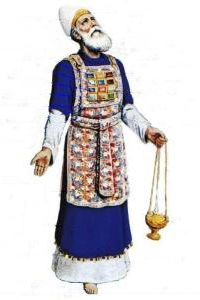
\includegraphics[width=50mm,scale=1.5]{Extras/Melchisedec.jpg}
\vspace{0.4in}  % Create a title for the document and write it in bold font
\LARGE{\textbf{\date}} % Again, do a line break
\linebreak 
% Create a subtitle \large{with Outlines, Statistics, Cross References, and Notes}
\vspace{0.5in}
\begin{flushleft}
\LARGE{Day \#35: Friday, 4 February 2022 LITE  \\}\vspace{0.25in}
\LARGE{Leviticus 10-12 Psalm 35 Proverb 4}
\end{flushleft}
\vspace{0.6in}
\bigskip

\normalsize{Xenia, Oh.\\}
\normalsize{created: \today}
\vspace{1.3in}

\end{flushright}
\end{titlepage}

%\titleJE
\newpage 
\tableofcontents\hypertarget{TOC}{}

\hyphenation{A-bim-e-lech bre-thren E-phra-im  Gib-e-o-nites Jer-u-sa-lem through-out Phil-i-stines The-o-phil-us Am-a-le-kites ven-geance Mesh-el-e-mi-ah onan-ism Phar-a-oh thoughts grev-ous-ness Hach-a-liah adul-ter-er Shad-rach}

%%%%%%%%%%%%%%%%% EXTRA COLORS
%%%%%%%%%%%%%%%%% EXTRA COLORS
%%%%%%%%%%%%%%%%% EXTRA COLORS
\definecolor{champagne}{rgb}{0.97,0.91,0.81}
\definecolor{bone}{rgb}{0.89,0.85,0.79}

\definecolor{ForestGreen}{rgb}{0.00,0.29,0.098}
\definecolor{GIVING}{cmyk}{1,0.0,0.72,.1}

\definecolor{MLPE}{cmyk}{1,1,0,.45}
\definecolor{SOCCER}{cmyk}{.77, 0, .42, .49}
\definecolor{PAYBILL}{cmyk}{0,0.83,0.76,0.07}
\definecolor{SERMON}{cmyk}{.14,.9,0,.30} % aka seance \href{http://www.flatuicolorpicker.com/purple-cmyk-color-model/}{seance}
\definecolor{BIBLE}{cmyk}{0,.17,.74,.17}
\definecolor{WORKBLUE}{cmyk}{1, .5, 0, .6}
\definecolor{myOrange}{cmyk}{0, .4, .98, .03}
\definecolor{myTan}{cmyk}{0.0,.07,.17,.10}
\definecolor{myRed}{cmyk}{0,1,1,0}
\definecolor{myWhite}{cmyk}{0,0,0,0}
\definecolor{BLUESoD}{cmyk}{.97,.84,0,.04}
\definecolor{WHITE}{cmyk}{0,0,0,0}
\definecolor{OLDGOLD}{cmyk}{0.05,0.3,1.00,0}
\definecolor{CASTLETON}{cmyk}{1,0,0.31,0.66}
\definecolor{cadmiumgreen}{rgb}{0.0, 0.42, 0.24}
\definecolor{jungle}{rgb}{0.203,0.4882,0.1718}
\definecolor{MYGOLD}{rgb}{1,.84,0}

\definecolor{MYLIGHTGRAY}{rgb}{.85,.85,.85}

\definecolor{codegreen}{rgb}{0,0.6,0}
\definecolor{codegray}{rgb}{0.5,0.5,0.5}
\definecolor{codepurple}{rgb}{0.58,0,0.82}
\definecolor{backcolour}{rgb}{0.95,0.95,0.92}


\mdfdefinestyle{MyFrame}{%
    linecolor=blue,
    outerlinewidth=2pt,
    roundcorner=5pt,
    innertopmargin=\baselineskip,
    innerbottommargin=\baselineskip,
    innerrightmargin=10pt,
    innerleftmargin=10pt,
    backgroundcolor=gray!25!white}


\mdfdefinestyle{MyFrame2}{%
    linecolor=black,
    outerlinewidth=2pt,
    roundcorner=5pt,
    innertopmargin=\baselineskip,
    innerbottommargin=\baselineskip,
    innerrightmargin=10pt,
    innerleftmargin=10pt,
    backgroundcolor=yellow!25!white}


%%%%%
%% for PFTTIS list
%%%%%

%%% And Joseph said unto
\index[PFTTIS]{And Joseph said unto!Genesis!Gen 40:008}
\index[PFTTIS]{And Joseph said unto!Genesis!Gen 40:012}
\index[PFTTIS]{And Joseph said unto!Genesis!Gen 41:025}
\index[PFTTIS]{And Joseph said unto!Genesis!Gen 42:014}
\index[PFTTIS]{And Joseph said unto!Genesis!Gen 42:018}
\index[PFTTIS]{And Joseph said unto!Genesis!Gen 44:015}
\index[PFTTIS]{And Joseph said unto!Genesis!Gen 45:003}
\index[PFTTIS]{And Joseph said unto!Genesis!Gen 45:004}
\index[PFTTIS]{And Joseph said unto!Genesis!Gen 46:031}
\index[PFTTIS]{And Joseph said unto!Genesis!Gen 48:009}
\index[PFTTIS]{And Joseph said unto!Genesis!Gen 48:018}
\index[PFTTIS]{And Joseph said unto!Genesis!Gen 50:019}
\index[PFTTIS]{And Joseph said unto!Genesis!Gen 50:024}


%%% a shadow
\index[PFTTIS]{a shadow!1Chronicles!1Chr 029:15}
\index[PFTTIS]{a shadow!Job!Job 008:09}
\index[PFTTIS]{a shadow!Job!Job 014:02}
\index[PFTTIS]{a shadow!Job!Job 017:07}
\index[PFTTIS]{a shadow!Psalm!Psa 102:011}
\index[PFTTIS]{a shadow!Psalm!Psa 144:004}
\index[PFTTIS]{a shadow!Ecclesiastes!Eccl 006:012}
\index[PFTTIS]{a shadow!Ecclesiastes!Eccl 008:013}
\index[PFTTIS]{a shadow!Isaiah!Isa 04:006}
\index[PFTTIS]{a shadow!Isaiah!Isa 25:004}
\index[PFTTIS]{a shadow!Jonah!Jnh 04:06}
\index[PFTTIS]{a shadow!Colossians!Col 02:017}
\index[PFTTIS]{a shadow!Hebews!Heb 10:001}

%%% blessed is the man
\index[PFTTIS]{blessed is the man!Psalm!Psa 001:001}
\index[PFTTIS]{blessed is the man!Psalm!Psa 032:002}
\index[PFTTIS]{blessed is the man!Psalm!Psa 034:008}
\index[PFTTIS]{blessed is the man!Psalm!Psa 065:004}
\index[PFTTIS]{blessed is the man!Psalm!Psa 084:005}
\index[PFTTIS]{blessed is the man!Psalm!Psa 084:012}
\index[PFTTIS]{blessed is the man!Psalm!Psa 094:012}
\index[PFTTIS]{blessed is the man!Psalm!Psa 112:001}
\index[PFTTIS]{blessed is the man!Proverbs!Pro 008:034}
\index[PFTTIS]{blessed is the man!Isaiah!Isa 056:002}
\index[PFTTIS]{blessed is the man!Jeremiah!Jer 017:007}
\index[PFTTIS]{blessed is the man!Romans!Rom 004:008}
\index[PFTTIS]{blessed is the man!James!Jam 001:012}


%%% carry them
\index[PFTTIS]{carry them!Leviticus!Lev 14:045}
\index[PFTTIS]{carry them!Numbers!Num 11:012}
\index[PFTTIS]{carry them!Joshua!Jsh 04:003}
\index[PFTTIS]{carry them!1Samuel!1Sam 20:040}
\index[PFTTIS]{carry them!1Kings!1Kng 08:046}
\index[PFTTIS]{carry them!2Chronicles!2Chr 06:036}
\index[PFTTIS]{carry them!Ezra!Ezra 05:015}
\index[PFTTIS]{carry them!Isaiah!Isa 40:011}
\index[PFTTIS]{carry them!Isaiah!Isa 41:016}
\index[PFTTIS]{carry them!Isaiah!Isa 57:013}
\index[PFTTIS]{carry them!Jeremiah!Jer 20:004}
\index[PFTTIS]{carry them!Jeremiah!Jer 20:005}
\index[PFTTIS]{carry them!Jeremiah!Jer 43:012}


\index[PFTTIS]{good tidings!2Samuel!2Sam 18:027}
\index[PFTTIS]{good tidings!1Kings!1Ki 01:042}
\index[PFTTIS]{good tidings!2Kings!2Ki 07:009 (2x)}
\index[PFTTIS]{good tidings!Isaiah!Isa 40:009 (2x)}
\index[PFTTIS]{good tidings!Isaiah!Isa 41:007}
\index[PFTTIS]{good tidings!Isaiah!Isa 52:007}
\index[PFTTIS]{good tidings!Isaiah!Isa 61:001}
\index[PFTTIS]{good tidings!Nahum!Nah 01:005}
\index[PFTTIS]{good tidings!Luke!Lk 02:010}
\index[PFTTIS]{good tidings!1Thessalonians!1Thess 03:006}


%%% dead body
\index[PFTTIS]{dead body!Leviticus!Lev 21:011}
\index[PFTTIS]{dead body!Numbers!Num 06:006}
\index[PFTTIS]{dead body!Numbers!Num 09:006}
\index[PFTTIS]{dead body!Numbers!Num 09:007}
\index[PFTTIS]{dead body!Numbers!Num 09:010}
\index[PFTTIS]{dead body!Numbers!Num 09:011}
\index[PFTTIS]{dead body!Numbers!Num 09:013}
\index[PFTTIS]{dead body!Numbers!Num 09:016}
\index[PFTTIS]{dead body!2Kings!2Ki 08:005}
\index[PFTTIS]{dead body!Isaiah!Isa 26:019}
\index[PFTTIS]{dead body!Jeremiah!Jer 26:023}
\index[PFTTIS]{dead body!Jeremiah!Jer 36:030}
\index[PFTTIS]{dead body!Haggai!Hag 02:013}

%%% great sea
\index[PFTTIS]{great sea!Numbers!Num 34:006}
\index[PFTTIS]{great sea!Numbers!Num 34:007}
\index[PFTTIS]{great sea!Joshua!Jos 01:004}
\index[PFTTIS]{great sea!Joshua!Jos 09:001}
\index[PFTTIS]{great sea!Joshua!Jos 15:012}
\index[PFTTIS]{great sea!Joshua!Jos 15:047}
\index[PFTTIS]{great sea!Joshua!Jos 23:004}
\index[PFTTIS]{great sea!Ezekiel!Eze 47:010}
\index[PFTTIS]{great sea!Ezekiel!Eze 47:015}
\index[PFTTIS]{great sea!Ezekiel!Eze 47:019}
\index[PFTTIS]{great sea!Ezekiel!Eze 47:020}
\index[PFTTIS]{great sea!Ezekiel!Eze 48:028}
\index[PFTTIS]{great sea!Daniel!Dan 07:002}


%%% have forsaken me
\index[PFTTIS]{have forsaken me!Judges!Jdg 10:013}
\index[PFTTIS]{have forsaken me!1Samuel!1Sam 08:008}
\index[PFTTIS]{have forsaken me!1Kings!1Ki 11:033}
\index[PFTTIS]{have forsaken me!2Kings!2Ki 22:017}
\index[PFTTIS]{have forsaken me!2Chronicles!2Chr 12:005}
\index[PFTTIS]{have forsaken me!2Chronicles!2Chr 34:025}
\index[PFTTIS]{have forsaken me!Jeremiah!Jer 01:016}
\index[PFTTIS]{have forsaken me!Jeremiah!Jer 02:013}
\index[PFTTIS]{have forsaken me!Jeremiah!Jer 05:007}
\index[PFTTIS]{have forsaken me!Jeremiah!Jer 05:019}
\index[PFTTIS]{have forsaken me!Jeremiah!Jer 16:011 (2x)}
\index[PFTTIS]{have forsaken me!Jeremiah!Jer 19:004}

%%% no king
\index[PFTTIS]{no king!Judges!Jdg 17:06}
\index[PFTTIS]{no king!Judges!Jdg 18:01}
\index[PFTTIS]{no king!Judges!Jdg 19:01}
\index[PFTTIS]{no king!Judges!Jdg 21:25}
\index[PFTTIS]{no king!1Kings!1Ki 22:47}
\index[PFTTIS]{no king!2Kings!2Ki 23:25}
\index[PFTTIS]{no king!Nehemiah!Neh 13:26}
\index[PFTTIS]{no king!Psalms!Psa 033:016}
\index[PFTTIS]{no king!Proverbs!Pro 30:27}
\index[PFTTIS]{no king!Daniel!Dan 02:10}
\index[PFTTIS]{no king!Hosea!Hos 10:03}
\index[PFTTIS]{no king!Micah!Mic 04:09}
\index[PFTTIS]{no king!John!Jhn 19:15}


%%% rebellious house
\index[PFTTIS]{rebellious house!Exodus!Exo 02:005}
\index[PFTTIS]{rebellious house!Exodus!Exo 02:006}
\index[PFTTIS]{rebellious house!Exodus!Exo 02:008}
\index[PFTTIS]{rebellious house!Exodus!Exo 03:009}
\index[PFTTIS]{rebellious house!Exodus!Exo 03:026}
\index[PFTTIS]{rebellious house!Exodus!Exo 03:027}
\index[PFTTIS]{rebellious house!Exodus!Exo 12:002 (2x)}
\index[PFTTIS]{rebellious house!Exodus!Exo 12:003}
\index[PFTTIS]{rebellious house!Exodus!Exo 12:009}
\index[PFTTIS]{rebellious house!Exodus!Exo 12:025}
\index[PFTTIS]{rebellious house!Exodus!Exo 17:012}
\index[PFTTIS]{rebellious house!Exodus!Exo 24:003}

%%% seek him
\index[PFTTIS]{seek him!Deuteronomy!Deu 04:029}\index[PFTTIS]{seek him!1Samuel!1Sam 23:025}
\index[PFTTIS]{seek him!1Chronicles!1Chr 28:009}
\index[PFTTIS]{seek him!2Chronicles!1Chr 15:002}
\index[PFTTIS]{seek him!Ezra!Ezr 08:022}
\index[PFTTIS]{seek him!Psalms!Psa 022:026}
\index[PFTTIS]{seek him!Psalms!Psa 024:006}
\index[PFTTIS]{seek him!Psalms!Psa 119:002}
\index[PFTTIS]{seek him!SoS!SoS 03:002}
\index[PFTTIS]{seek him!SoS!SoS 06:001}
\index[PFTTIS]{seek him!Hosea!Hos 07:010}
\index[PFTTIS]{seek him!Amos!Amo 05:008}
\index[PFTTIS]{seek him!Hebrews!Heb 11:0063}


%%% seek ye
\index[PFTTIS]{seek ye!Isaiah!Isa 34:016}
\index[PFTTIS]{seek ye!Isaiah!Isa 45:019}
\index[PFTTIS]{seek ye!Isaiah!Isa 55:006}
\index[PFTTIS]{seek ye!Amos!Amos 5:004}
\index[PFTTIS]{seek ye!John!John 1:38}
\index[PFTTIS]{seek ye!John!John 18:4}
\index[PFTTIS]{seek ye!John!John 18:7}
\index[PFTTIS]{seek ye!Matthew!Matt 6:33}
\index[PFTTIS]{seek ye!Numbers!Num 16:10}
\index[PFTTIS]{seek ye!Luke!Luke 12:31}
\index[PFTTIS]{seek ye!Luke!Luke 24:5}
\index[PFTTIS]{seek ye!Psalm!Psa 27:8}
\index[PFTTIS]{seek ye!Zephaniah!Zeph 2:3}

%%% the uncircumcised
\index[PFTTIS]{the uncircumcised!Genesis!Gen 17:014}
\index[PFTTIS]{the uncircumcised!Judges!Jdg 14:003}
\index[PFTTIS]{the uncircumcised!Judges!Jdg 15:018}
\index[PFTTIS]{the uncircumcised!2Samuel!2Sam 01:020}
\index[PFTTIS]{the uncircumcised!Isaiah!Isa 02:001}
\index[PFTTIS]{the uncircumcised!Jeremiah!Jer 09:025}
\index[PFTTIS]{the uncircumcised!Ezekiel!Eze 28:010}
\index[PFTTIS]{the uncircumcised!Ezekiel!Eze 31:018}
\index[PFTTIS]{the uncircumcised!Ezekiel!Eze 32:019}
\index[PFTTIS]{the uncircumcised!Ezekiel!Eze 32:027}
\index[PFTTIS]{the uncircumcised!Ezekiel!Eze 32:028}
\index[PFTTIS]{the uncircumcised!Ezekiel!Eze 32:029}
\index[PFTTIS]{the uncircumcised!Ezekiel!Eze 32:032}

%%% worship him
\index[PFTTIS]{worship him!Psalms!Psa 97:007}
\index[PFTTIS]{worship him!Zephaniah!Zeph 02:011}
\index[PFTTIS]{worship him!Matthew!Matt 02:002}
\index[PFTTIS]{worship him!Matthew!Matt 02:008}
\index[PFTTIS]{worship him!John!John 04:023}
\index[PFTTIS]{worship him!John!John 04:024 (2x)} 
\index[PFTTIS]{worship him!Acts!Acts 17:023}
\index[PFTTIS]{worship him!Hebrews!Heb 01:006}
\index[PFTTIS]{worship him!Revelation!Rev 04:010}
\index[PFTTIS]{worship him!Revelation!Rev 13:008}
\index[PFTTIS]{worship him!Revelation!Rev 14:007}
\index[PFTTIS]{worship him!Revelation!Rev 19:010}


%%%%%
%% for PFTTIS list
%%%%%

%%% afflictions
\index[WFTTIS]{afflictions!Psalms!Psa 34:019}
\index[WFTTIS]{afflictions!Psalms!Psa 132:001}
\index[WFTTIS]{afflictions!Acts!Acts 07:010}
\index[WFTTIS]{afflictions!Acts!Acts 20:023}
\index[WFTTIS]{afflictions!2Corinthians!2Cor 06:004}
\index[WFTTIS]{afflictions!Colossians!Col 01:024}
\index[WFTTIS]{afflictions!1Thessalonians!1Thess 03:003}
\index[WFTTIS]{afflictions!2Timothy!2Tim 01:008}
\index[WFTTIS]{afflictions!2Timothy!2Tim 03:011}
\index[WFTTIS]{afflictions!2Timothy!2Tim 04:005}
\index[WFTTIS]{afflictions!Hebrews!Heb 10:032}
\index[WFTTIS]{afflictions!Hebrews!Heb 10:033}
\index[WFTTIS]{afflictions!1Peter!1Pet 05:009}

%%% acsend
\index[WFTTIS]{acsend!Joshua!Jos 06:05}
\index[WFTTIS]{acsend!Psalm!Psa 024:003}
\index[WFTTIS]{acsend!Psalm!Psa 135:007}
\index[WFTTIS]{acsend!Psalm!Psa 139:008}
\index[WFTTIS]{acsend!Isaiah!Isa 14:013}
\index[WFTTIS]{acsend!Isaiah!Isa 14:014}
\index[WFTTIS]{acsend!Jeremiah!Jer 10:013}
\index[WFTTIS]{acsend!Jeremiah!Jer 51:016}
\index[WFTTIS]{acsend!Ezekiel!Eze 38:009}
\index[WFTTIS]{acsend!John!John 06:062}
\index[WFTTIS]{acsend!John!John 20:017}
\index[WFTTIS]{acsend!Romans!Rom 10:006}
\index[WFTTIS]{acsend!Revelation!Rev 17:008}

%%% Assyrian
\index[WFTTIS]{Assyrian!Isaiah!Isa 10:005}
\index[WFTTIS]{Assyrian!Isaiah!Isa 10:024}
\index[WFTTIS]{Assyrian!Isaiah!Isa 14:025}
\index[WFTTIS]{Assyrian!Isaiah!Isa 19:023}
\index[WFTTIS]{Assyrian!Isaiah!Isa 23:013}
\index[WFTTIS]{Assyrian!Isaiah!Isa 30:031}
\index[WFTTIS]{Assyrian!Isaiah!Isa 31:008}
\index[WFTTIS]{Assyrian!Isaiah!Isa 52:004}
\index[WFTTIS]{Assyrian!Ezekiel!Eze 31:003}
\index[WFTTIS]{Assyrian!Hosea!Hos 05:013}
\index[WFTTIS]{Assyrian!Hosea!Hos 11:005}
\index[WFTTIS]{Assyrian!Micah!Hos 05:005}
\index[WFTTIS]{Assyrian!Micah!Hos 05:006}

%%% blot
\index[WFTTIS]{blot!Exodus!Exo 32:032}
\index[WFTTIS]{blot!Exodus!Exo 32:033}
\index[WFTTIS]{blot!Numbers!Num 05:026}
\index[WFTTIS]{blot!Deuteronomy!Deut 09:014}
\index[WFTTIS]{blot!Deuteronomy!Deut 25:019}
\index[WFTTIS]{blot!Deuteronomy!Deut 29:020}
\index[WFTTIS]{blot!2Kings!2Ki 14:027}
\index[WFTTIS]{blot!Job!Job 31:007}
\index[WFTTIS]{blot!Psalms!Psa 51:001}
\index[WFTTIS]{blot!Psalms!Psa 51:009}
\index[WFTTIS]{blot!Proverbs!Pro 09:007}
\index[WFTTIS]{blot!Jeremiah!Jer 18:023}
\index[WFTTIS]{blot!Revelation!Rev 03:005}


%%% chain
\index[WFTTIS]{chain!Genesis!Gen 41:042}
\index[WFTTIS]{chain!1Kings!1Ki 07:017}
\index[WFTTIS]{chain!Psalms!Psa 73:006}
\index[WFTTIS]{chain!SoS!Sos 04:009}
\index[WFTTIS]{chain!Lamentations!Lam 03:007}
\index[WFTTIS]{chain!Ezekiel!Eze 07:023}
\index[WFTTIS]{chain!Ezekiel!Eze 16:011}
\index[WFTTIS]{chain!Daniel!Dan 05:007}
\index[WFTTIS]{chain!Daniel!Dan 05:016}
\index[WFTTIS]{chain!Daniel!Dan 05:029}
\index[WFTTIS]{chain!Acts!Acts 28:020}
\index[WFTTIS]{chain!2Timothy!2Tim 01:016}
\index[WFTTIS]{chain!Revelation!Rev 20:001}


%%% controversy
\index[WFTTIS]{controversy!Deuteronomy!Deu 17:008}
\index[WFTTIS]{controversy!Deuteronomy!Deu 19:017}
\index[WFTTIS]{controversy!Deuteronomy!Deu 21:005}
\index[WFTTIS]{controversy!Deuteronomy!Deu 25:001}
\index[WFTTIS]{controversy!2Samuel!2Sam 15:002}
\index[WFTTIS]{controversy!Isaiah!Isa 34:008}
\index[WFTTIS]{controversy!Jeremiah!Jer 25:031}
\index[WFTTIS]{controversy!Ezekiel!Eze 44:024}
\index[WFTTIS]{controversy!Hosea!Hos 04:001}
\index[WFTTIS]{controversy!Hosea!Hos 12:002}
\index[WFTTIS]{controversy!Micah!Mic 06:002 (2x)}
\index[WFTTIS]{controversy!1Timothy!1Tim 03:016}


%%% Dagon/Dagon's
\index[WFTTIS]{Dagon!Judges!Jdg 16:023}
\index[WFTTIS]{Dagon!1Samuel!1Sam 05:002 (2x)}
\index[WFTTIS]{Dagon!1Samuel!1Sam 05:003 (2x)}
\index[WFTTIS]{Dagon!1Samuel!1Sam 05:004 (3x)}
\index[WFTTIS]{Dagon!1Samuel!1Sam 05:005 (3x)}
\index[WFTTIS]{Dagon!1Samuel!1Sam 05:007}
\index[WFTTIS]{Dagon!1Chronicles!1Chr 10:010}

%%% disobedient
\index[WFTTIS]{disobedient!1Kings!1Ki 13:026}
\index[WFTTIS]{disobedient!Nehemiah!Neh 09:026}
\index[WFTTIS]{disobedient!Luke!Luke 01:017}
\index[WFTTIS]{disobedient!Acts!Acts 26:019}
\index[WFTTIS]{disobedient!Romans!Rom 01:030}
\index[WFTTIS]{disobedient!Romans!Rom 10:021}
\index[WFTTIS]{disobedient!1Timothy!1Tim 01:009}
\index[WFTTIS]{disobedient!2Timothy!2Tim 03:002}
\index[WFTTIS]{disobedient!Titus!Titus 01:016}
\index[WFTTIS]{disobedient!Titus!Titus 03:003}
\index[WFTTIS]{disobedient!1Peter!1Pet 02:007}
\index[WFTTIS]{disobedient!1Peter!1Pet 02:008}
\index[WFTTIS]{disobedient!1Peter!1Pet 03:020}


%%% doubt
\index[WFTTIS]{doubt!Genesis!Gen 37:033}
\index[WFTTIS]{doubt!Deuteronomy!Deu 28:066}
\index[WFTTIS]{doubt!Job!Job 12:002}
\index[WFTTIS]{doubt!Matthew!Matt 14:031}
\index[WFTTIS]{doubt!Matthew!Matt 21:021}
\index[WFTTIS]{doubt!Mark!Mk 11:023}
\index[WFTTIS]{doubt!Luke!Lk 11:020}
\index[WFTTIS]{doubt!John!Jhn 10:024}
\index[WFTTIS]{doubt!Acts!Acts 02:012}
\index[WFTTIS]{doubt!Acts!Acts 28:004}
\index[WFTTIS]{doubt!1Corinthians!1Cor 09:010}
\index[WFTTIS]{doubt!Galatians!Gal 04:020}
\index[WFTTIS]{doubt!1John!1Jhn 02:019}


%%% dungeon
\index[WFTTIS]{dungeon!Genesis!Gen 40:015}
\index[WFTTIS]{dungeon!Genesis!Gen 41:014}
\index[WFTTIS]{dungeon!Exodus!Exo 12:029}
\index[WFTTIS]{dungeon!Jeremiah!Jer 37:016}
\index[WFTTIS]{dungeon!Jeremiah!Jer 38:006 (2x)}
\index[WFTTIS]{dungeon!Jeremiah!Jer 38:007}
\index[WFTTIS]{dungeon!Jeremiah!Jer 38:009}
\index[WFTTIS]{dungeon!Jeremiah!Jer 38:010}
\index[WFTTIS]{dungeon!Jeremiah!Jer 38:011}
\index[WFTTIS]{dungeon!Jeremiah!Jer 38:013}
\index[WFTTIS]{dungeon!Lamentations!Lam 03:053}
\index[WFTTIS]{dungeon!Lamentations!Lam 03:055}


%%% error
\index[WFTTIS]{error!2Samuel!2Sam 06:007}
\index[WFTTIS]{error!Job!Job 19:004}
\index[WFTTIS]{error!Ecclesiastes!Ecc 05:006}
\index[WFTTIS]{error!Ecclesiastes!Ecc 10:005}
\index[WFTTIS]{error!Isaiah!Isa 32:006}
\index[WFTTIS]{error!Daniel!Dan 06:004}
\index[WFTTIS]{error!Matthew!Matt 27:064}
\index[WFTTIS]{error!Romans!Rom 01:027}
\index[WFTTIS]{error!James!Jam 05:020}
\index[WFTTIS]{error!2Peter!2Pet 02:018}
\index[WFTTIS]{error!2Peter!2Pet 03:017}
\index[WFTTIS]{error!1John!1Jn 04:006}
\index[WFTTIS]{error!Jude!Jude 01:011}

%%% fourish
\index[WFTTIS]{fourish!Psalms!Psa 072:007}
\index[WFTTIS]{fourish!Psalms!Psa 072:016}
\index[WFTTIS]{fourish!Psalms!Psa 092:007}
\index[WFTTIS]{fourish!Psalms!Psa 092:012}
\index[WFTTIS]{fourish!Psalms!Psa 092:013}
\index[WFTTIS]{fourish!Psalms!Psa 132:018}
\index[WFTTIS]{fourish!Proverbs!Pro 11:28}
\index[WFTTIS]{fourish!Proverbs!Pro 14:11}
\index[WFTTIS]{fourish!Ecclesiastes!Ecc 12:05}
\index[WFTTIS]{fourish!SongOfSolomon!SOS 07:12}
\index[WFTTIS]{fourish!Isaiah!Isa 17:11}
\index[WFTTIS]{fourish!Isaiah!Isa 66:14}
\index[WFTTIS]{fourish!Ezekiel!Eze 17:24}




%%% giants
\index[WFTTIS]{giants!Genesis!Gen 06:004}
\index[WFTTIS]{giants!Numbers!Num 13:033}
\index[WFTTIS]{giants!Deuteronomy!Deut 02:011}
\index[WFTTIS]{giants!Deuteronomy!Deut 02:021}
\index[WFTTIS]{giants!Deuteronomy!Deut 03:011}
\index[WFTTIS]{giants!Deuteronomy!Deut 03:013}
\index[WFTTIS]{giants!Joshua!Josh 12:004}
\index[WFTTIS]{giants!Joshua!Josh 13:012}
\index[WFTTIS]{giants!Joshua!Josh 15:008}
\index[WFTTIS]{giants!Joshua!Josh 17:015}
\index[WFTTIS]{giants!Joshua!Josh 16:016}

%%% good man
\index[WFTTIS]{good man!2 Samuel!2Sa 18:27}
%(1) Psalms 37:23 [5]
%(1) Psalms 112:5 [2]
%(1) Proverbs 12:2 [2]
%(1) Proverbs 13:22 [2]
%(1) Proverbs 14:14 [14]
%(1) Micah 7:2 [2]
%(1) Matthew 12:35 [2]
%(1) Luke 6:45 [2]
%(1) Luke 23:50 [15]
%(1) John 7:12 [17]
%(1) Acts 11:24 [5]
%(1) Romans 5:7 [14]

%%% Hinnom
\index[WFTTIS]{Hinnom!Joshua!Jsh 15:008}
\index[WFTTIS]{Hinnom!Joshua!Jsh 18:016}
\index[WFTTIS]{Hinnom!2Kings!2Ki 23:010}
\index[WFTTIS]{Hinnom!2Chronicles!2Chr 28:003}
\index[WFTTIS]{Hinnom!2Chronicles!2Chr 33:006}
\index[WFTTIS]{Hinnom!Nehemiah!Neh 11:030}
\index[WFTTIS]{Hinnom!Jeremiah!Jer 07:031}
\index[WFTTIS]{Hinnom!Jeremiah!Jer 07:032}
\index[WFTTIS]{Hinnom!Jeremiah!Jer 19:002}
\index[WFTTIS]{Hinnom!Jeremiah!Jer 19:006}
\index[WFTTIS]{Hinnom!Jeremiah!Jer 32:035}

%%% inclined
\index[WFTTIS]{inclined!Judges!Jdg 09:003}
\index[WFTTIS]{inclined!Psalms!Psa 040:001}
\index[WFTTIS]{inclined!Psalms!Psa 116:002}
\index[WFTTIS]{inclined!Psalms!Psa 119:112}
\index[WFTTIS]{inclined!Proverbs!Pro 05:13}
\index[WFTTIS]{inclined!Jeremiah!Jer 07:24}
\index[WFTTIS]{inclined!Jeremiah!Jer 07:26}
\index[WFTTIS]{inclined!Jeremiah!Jer 11:08}
\index[WFTTIS]{inclined!Jeremiah!Jer 17:23}
\index[WFTTIS]{inclined!Jeremiah!Jer 25:04}
\index[WFTTIS]{inclined!Jeremiah!Jer 34:14}
\index[WFTTIS]{inclined!Jeremiah!Jer 35:15}
\index[WFTTIS]{inclined!Jeremiah!Jer 44:05}


%%% laughed
\index[WFTTIS]{laughed!Genesis!Gen 17:017}
\index[WFTTIS]{laughed!Genesis!Gen 18:012}
\index[WFTTIS]{laughed!Genesis!Gen 18:015}
\index[WFTTIS]{laughed!2Kings!2Ki 19:021}
\index[WFTTIS]{laughed!2Chronicles!2Chr 30:010}
\index[WFTTIS]{laughed!Nehemiah!Neh 02:019}
\index[WFTTIS]{laughed!Job!Job 12:004}
\index[WFTTIS]{laughed!Job!Job 29:024}
\index[WFTTIS]{laughed!Isaiah!Isa 37:022}
\index[WFTTIS]{laughed!Ezekiel!Ezek 23:032}
\index[WFTTIS]{laughed!Matthew!Matt 09:024}
\index[WFTTIS]{laughed!Mark!Mk 05:040}
\index[WFTTIS]{laughed!Luke!Lk 08:053}

%%% liar
\index[WFTTIS]{liar!Job!Job 24:025}
\index[WFTTIS]{liar!Proverbs!Pro 17:004}
\index[WFTTIS]{liar!Proverbs!Pro 19:022}
\index[WFTTIS]{liar!Proverbs!Pro 30:006}
\index[WFTTIS]{liar!Jeremiah!Jer 15:018}
\index[WFTTIS]{liar!John!Jhn 08:044}
\index[WFTTIS]{liar!John!Jhn 08:055}
\index[WFTTIS]{liar!Romans!Rom 03:004}
\index[WFTTIS]{liar!1John!1Jhn 01:010}
\index[WFTTIS]{liar!1John!1Jhn 02:004}
\index[WFTTIS]{liar!1John!1Jhn 02:022}
\index[WFTTIS]{liar!1John!1Jhn 04:020}
\index[WFTTIS]{liar!1John!1Jhn 05:010}

%%% palsy
\index[WFTTIS]{palsy!Matthew!Matt 04:024}
\index[WFTTIS]{palsy!Matthew!Matt 08:006}
\index[WFTTIS]{palsy!Matthew!Matt 09:002}
\index[WFTTIS]{palsy!Matthew!Matt 09:006}
\index[WFTTIS]{palsy!Mark!Mk 02:003}
\index[WFTTIS]{palsy!Mark!Mk 02:004}
\index[WFTTIS]{palsy!Mark!Mk 02:005}
\index[WFTTIS]{palsy!Mark!Mk 02:009}
\index[WFTTIS]{palsy!Mark!Mk 02:010}
\index[WFTTIS]{palsy!Luke!Lk 05:018}
\index[WFTTIS]{palsy!Luke!Lk 05:024}
\index[WFTTIS]{palsy!Acts!Acts 09:033}

%%% Profitable
\index[WFTTIS]{profitable!Job!Job 22:002 (2x)}
\index[WFTTIS]{profitable!Ecclesiastes!Ecc 10:010}
\index[WFTTIS]{profitable!Isaiah!Isa 44:010}
\index[WFTTIS]{profitable!Jeremiah!Jer 13:007}
\index[WFTTIS]{profitable!Matthew!Matt 05:029}
\index[WFTTIS]{profitable!Matthew!Matt 05:030}
\index[WFTTIS]{profitable!Acts!Acts 20:020}
\index[WFTTIS]{profitable!1Timothy!1Tim 04:008}
\index[WFTTIS]{profitable!2Timothy!2Tim 03:016}
\index[WFTTIS]{profitable!2Timothy!2Tim 04:011}
\index[WFTTIS]{profitable!Titus!Titus 03:008}
\index[WFTTIS]{profitable!Philemon!Phlm 01:011}

%%% Rechab
\index[WFTTIS]{Rechab!2Samuel!2Sam 04:002}
\index[WFTTIS]{Rechab!2Samuel!2Sam 04:005}
\index[WFTTIS]{Rechab!2Samuel!2Sam 04:006}
\index[WFTTIS]{Rechab!2Samuel!2Sam 04:009}
\index[WFTTIS]{Rechab!2KIngs!2Ki 10:015}
\index[WFTTIS]{Rechab!2KIngs!2Ki 10:023}
\index[WFTTIS]{Rechab!1Chronicles!1Chr 02:055}
\index[WFTTIS]{Rechab!Nehemiah!Neh 03:014}
\index[WFTTIS]{Rechab!Jeremiah!Jer 35:006}
\index[WFTTIS]{Rechab!Jeremiah!Jer 35:008}
\index[WFTTIS]{Rechab!Jeremiah!Jer 35:014}
\index[WFTTIS]{Rechab!Jeremiah!Jer 35:016}
\index[WFTTIS]{Rechab!Jeremiah!Jer 35:019}

%%% serpents
\index[WFTTIS]{serpents!Exodus!Exo 07:012}
\index[WFTTIS]{serpents!Numbers!Num 21:006}
\index[WFTTIS]{serpents!Numbers!Num 21:007}
\index[WFTTIS]{serpents!Deuteronomy!Deu 08:015}
\index[WFTTIS]{serpents!Deuteronomy!Deu 32:024}
\index[WFTTIS]{serpents!Jeremiah!Jer 08:017}
\index[WFTTIS]{serpents!Matthew!Matt 10:016}
\index[WFTTIS]{serpents!Matthew!Matt 23:033}
\index[WFTTIS]{serpents!Mark!Mk 16:018}
\index[WFTTIS]{serpents!Luke!Lk 10:019}
\index[WFTTIS]{serpents!1Corinthians!1Cor 10:009}
\index[WFTTIS]{serpents!James!Jas 03:007}
\index[WFTTIS]{serpents!Revelation!Rev 09:019}

%%% short
\index[WFTTIS]{short!Numbers!Num 11:023}
\index[WFTTIS]{short!2Kings!2Ki 10:032}
\index[WFTTIS]{short!Job!Job 17:012}
\index[WFTTIS]{short!Job!Job 20:005}
\index[WFTTIS]{short!Psalms!Psa 89:047}
\index[WFTTIS]{short!Romans!Rom 03:023}
\index[WFTTIS]{short!Romans!Rom 09:028  (2x)}
\index[WFTTIS]{short!1Corinthians!1Cor 07:029}
\index[WFTTIS]{short!1Thessalonians!1Thess 02:017}
\index[WFTTIS]{short!Hebrews!Heb 04:001}
\index[WFTTIS]{short!Revelation!Rev 12:012}
\index[WFTTIS]{short!Revelation!Rev 17:010}

%%% smiteth
\index[WFTTIS]{smiteth!Exodus!Exo 21:012}
\index[WFTTIS]{smiteth!Exodus!Exo 21:15}
\index[WFTTIS]{smiteth!Deuteronomy!Dt 25:11}
\index[WFTTIS]{smiteth!Deuteronomy!Dt 27:24}
\index[WFTTIS]{smiteth!Joshua!Jsh 15:16}
\index[WFTTIS]{smiteth!Judges!Jdg 15:16}
\index[WFTTIS]{smiteth!2 Samuel!2Sa 05:08}
\index[WFTTIS]{smiteth!1Chronicles!1Chr 11:06}
\index[WFTTIS]{smiteth!Job!1Chr 26:12}
\index[WFTTIS]{smiteth!Isaiah!Isa 09:13}
\index[WFTTIS]{smiteth!Lamentations!Lam 03:30}
\index[WFTTIS]{smiteth!Ezekiel!Eze 07:09}
\index[WFTTIS]{smiteth!Luke!Lk 06:29}



%%% vanities
\index[WFTTIS]{vanities!Deuteronomy!Deut 21:021}
\index[WFTTIS]{vanities!1Kings!1Ki 16:013}
\index[WFTTIS]{vanities!1Kings!1Ki 16:026}
\index[WFTTIS]{vanities!Psalms!Psa 031:006}
\index[WFTTIS]{vanities!Ecclesiastes!Ecc 01:002 (2x)}
\index[WFTTIS]{vanities!Ecclesiastes!Ecc 05:007}
\index[WFTTIS]{vanities!Ecclesiastes!Ecc 12:008}
\index[WFTTIS]{vanities!Jeremiah!Jer 08:019}
\index[WFTTIS]{vanities!Jeremiah!Jer 10:008}
\index[WFTTIS]{vanities!Jeremiah!Jer 14:022}
\index[WFTTIS]{vanities!Jonah!Jnh 02:008}
\index[WFTTIS]{vanities!Acts!Acts 14:015}



%%%%%
%% for PFTTIS list
%%%%%

%%% worm
\index[WFITV]{worm!Exodus!Exo 16:024}
\index[WFITV]{worm!Job!Job 17:014}
\index[WFITV]{worm!Job!Job 24:029}
\index[WFITV]{worm!Job!Job 25:005 (2x)}
\index[WFITV]{worm!Psalms!Psa 022:006}
\index[WFITV]{worm!Isaiah!Isa 14:011}
\index[WFITV]{worm!Isaiah!Isa 41:014}
\index[WFITV]{worm!Isaiah!Isa 51:008}
\index[WFITV]{worm!Isaiah!Isa 66:024}
\index[WFITV]{worm!Jonah!Jnh 04:007}
\index[WFITV]{worm!Mark!Mk 09:044}
\index[WFITV]{worm!Mark!Mk 09:046}
\index[WFITV]{worm!Mark!Mk 09:048}


%\subsubsection{Title}
%\textbf{Introduction:} Isaiah 46 
%\index[speaker]{Speaker!Isaiah 49 (Title}
%\index[series]{Book (Speaker)!IPassage (Title)}
%\index[date]{2017/07/09!Isaiah 49 (Title)}
%\begin{compactenum}[I.]
%    \item  \textbf{Point} \index[scripture]{Isaiah!IPassage} (IPassage)
%\end{compactenum}




  
%%%%%%%%%%%%%%%%%%%%%%%%%%%

%\input{02OT-Exodus/ExodusIntroduction}

\newpage
\begin{figure}
\begin{center}
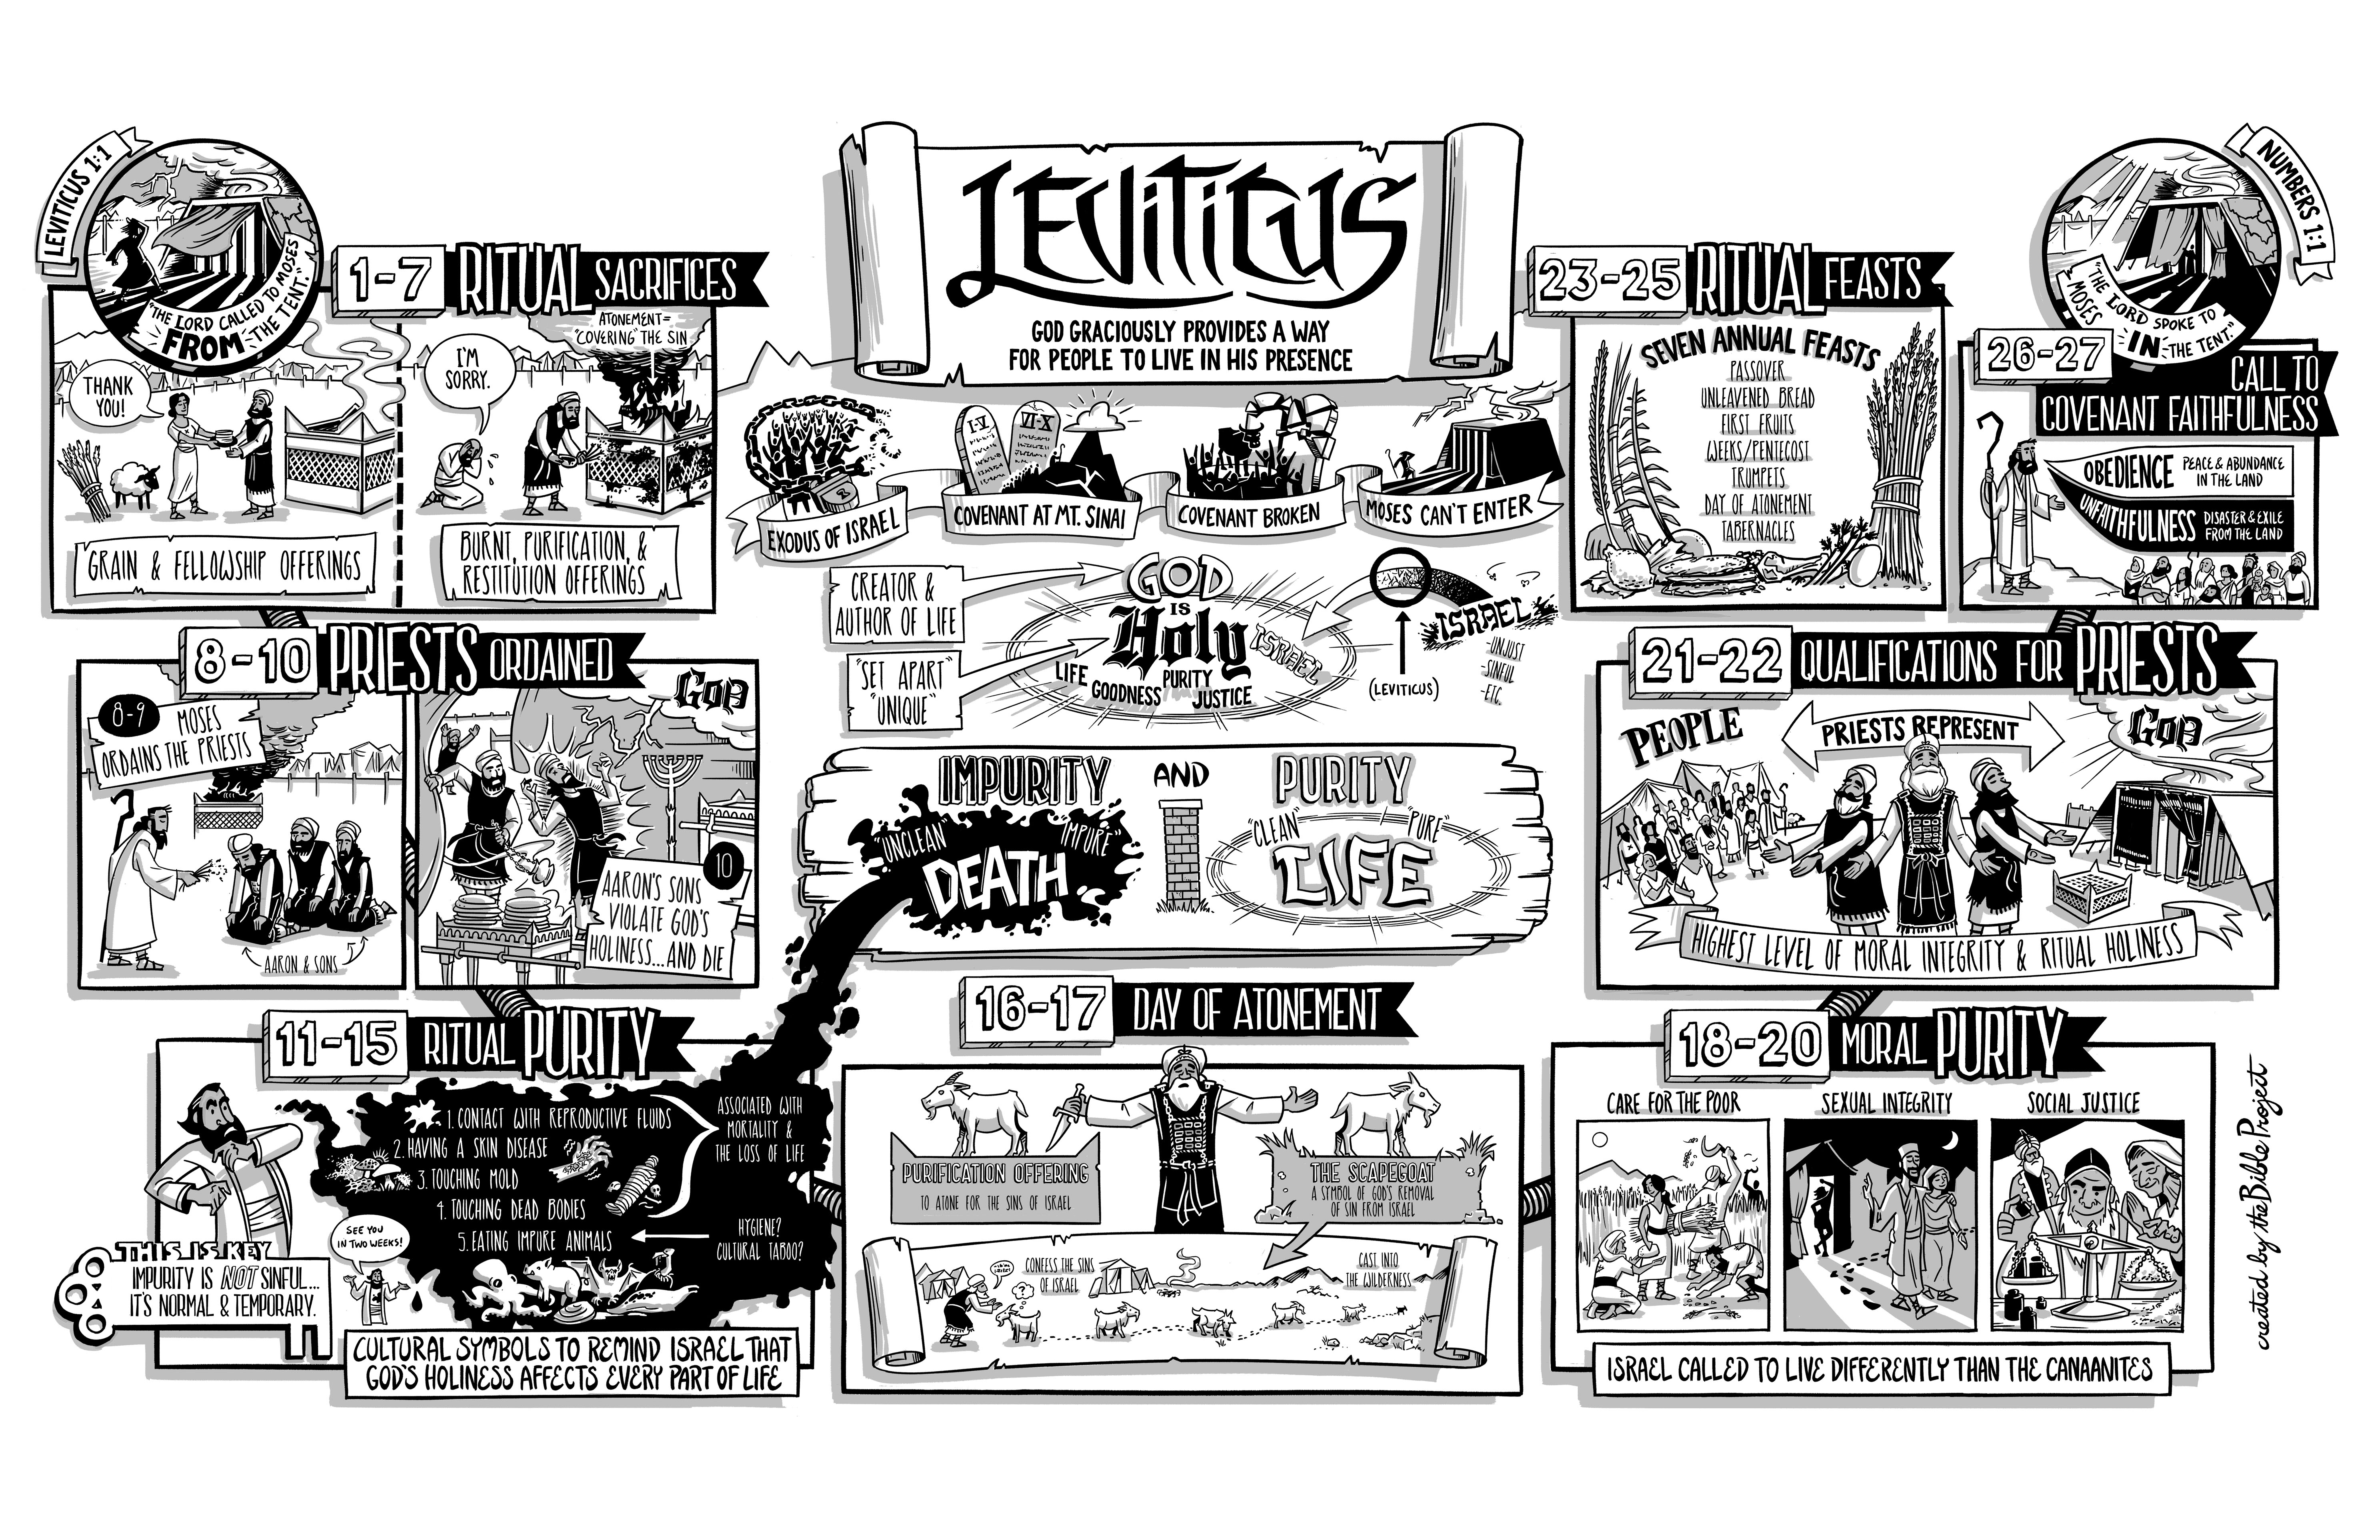
\includegraphics[scale=0.5, angle=90]{03OT-Leviticus/References/BibleProject-Leviticus.jpg}
\caption[Leviticus from the Bible Project]{Leviticus from the Bible Project}
\label{fig:Leviticus from the Bible Project}
\end{center}
\end{figure}

\newpage
\begin{figure}
\begin{center}
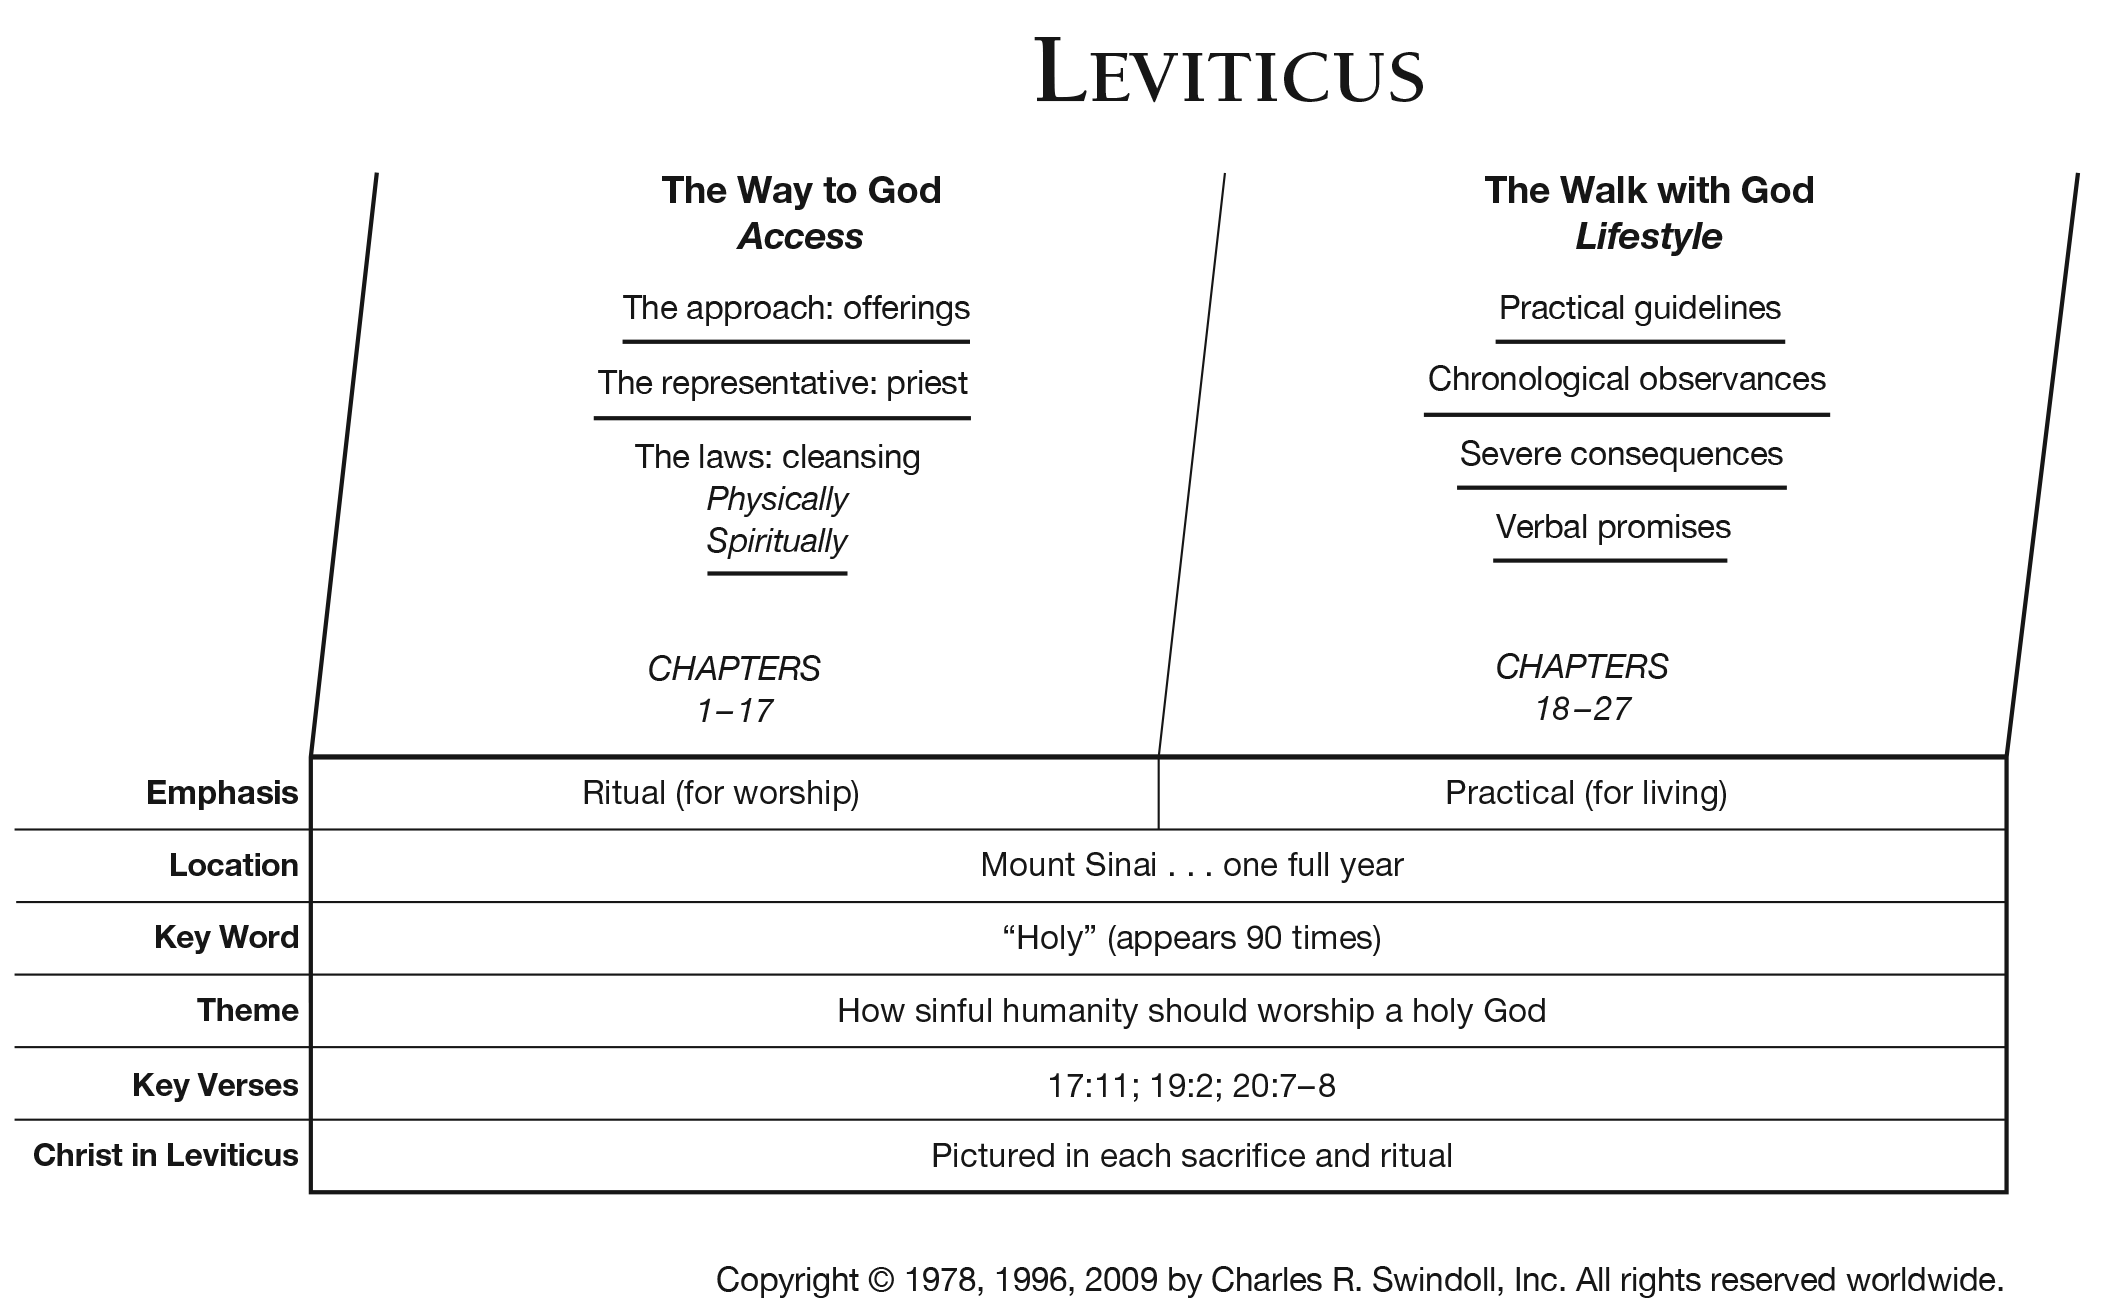
\includegraphics[scale=0.3, angle=90]{03OT-Leviticus/References/Swindoll-Leviticus.png}
\caption[Leviticus by Swindoll]{Leviticus by Swindoll}
\label{fig:Leviticus by Swindoll}
\end{center}
\end{figure}

\newpage
\begin{figure}
\begin{center}
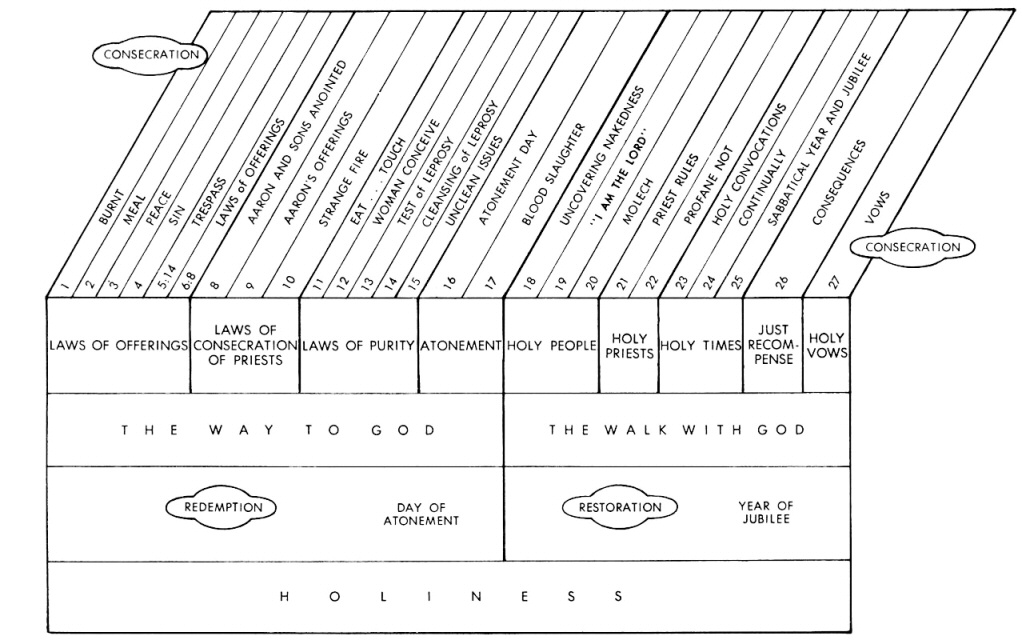
\includegraphics[scale=2, angle=90]{03OT-Leviticus/References/Jensen-Leviticus.png}
\caption[Leviticus by Jensen]{Leviticus by Jensen}
\label{fig:Leviticus by Jensen}
\end{center}
\end{figure}

\newpage
\begin{figure}
\begin{center}
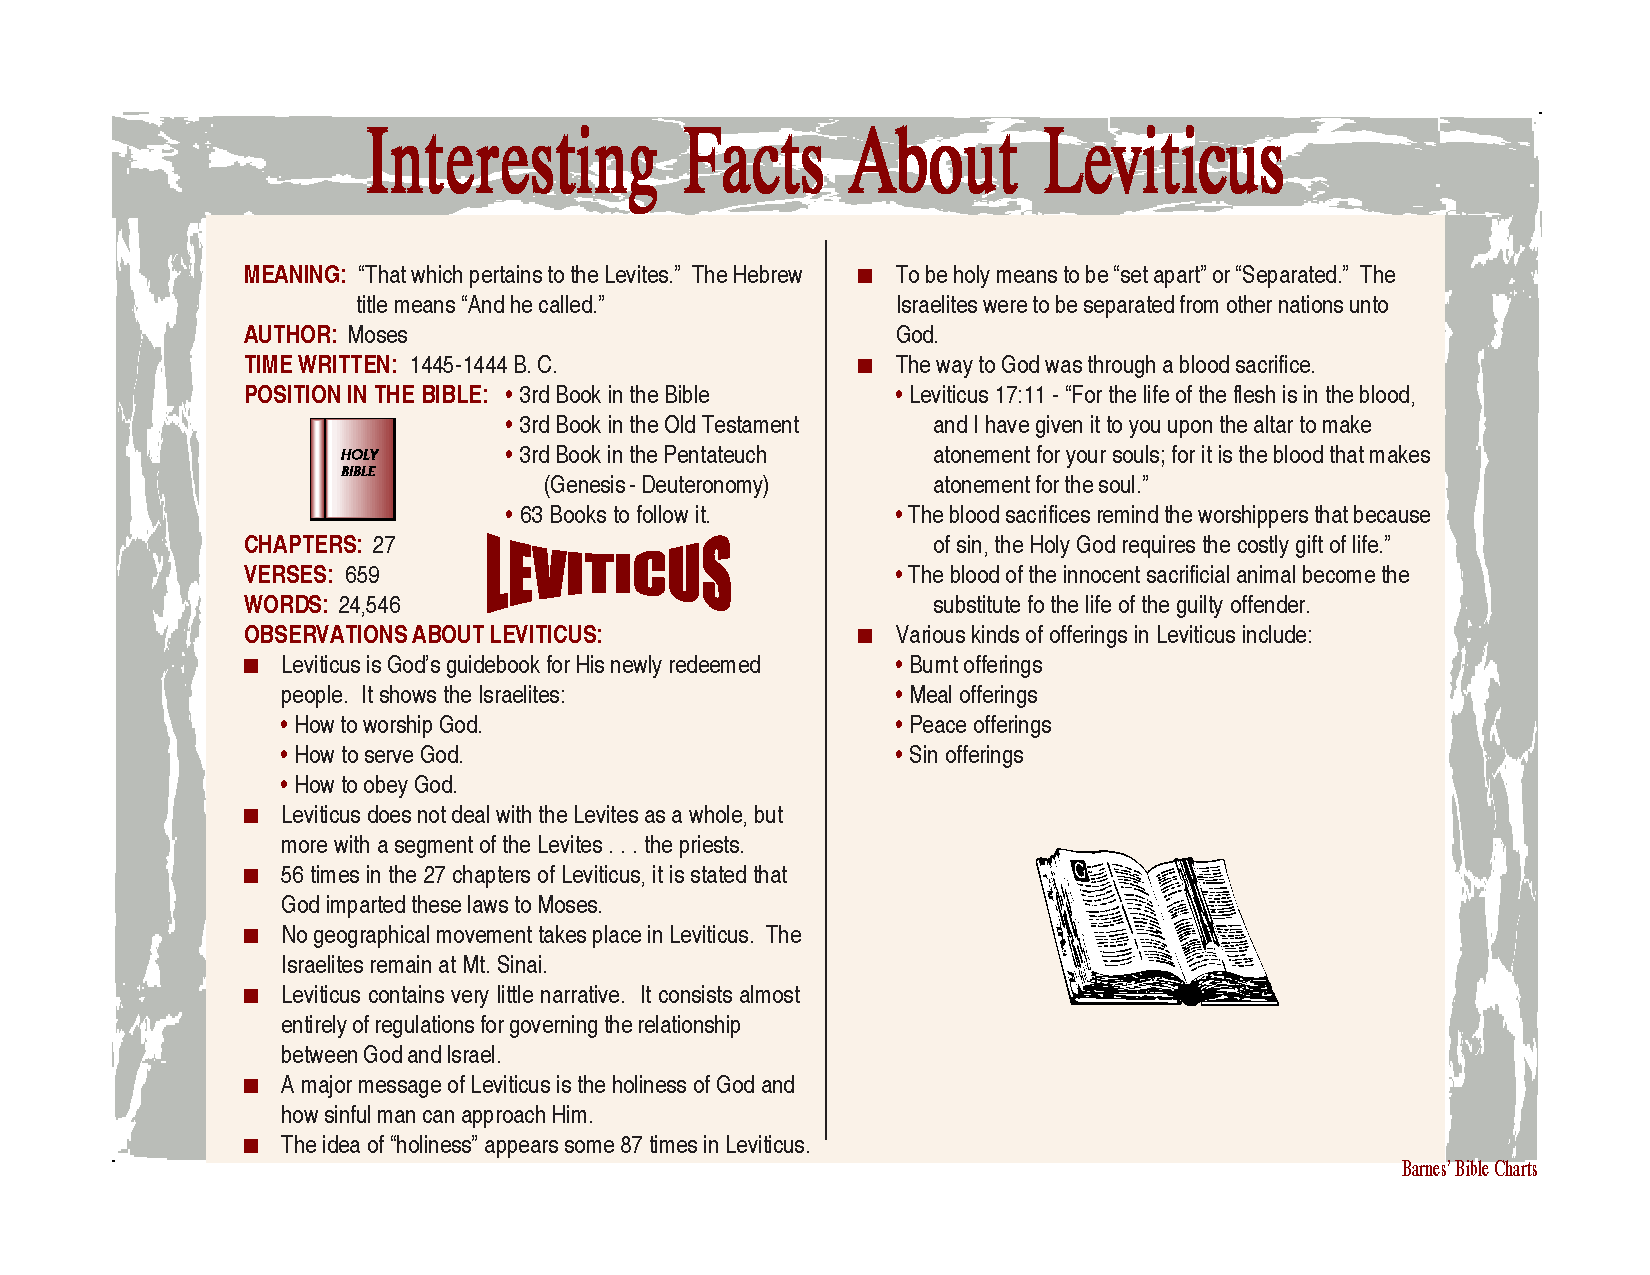
\includegraphics[scale=0.6, angle=90]{03OT-Leviticus/References/interestingfactsaboutleviticus.pdf}
\caption[Interesting Facts About Leviticus]{Interesting Facts About Leviticus}
\label{fig:Interesting Facts About Leviticus}
\end{center}
\end{figure}




\chapter{Leviticus 10}

\begin{figure}
  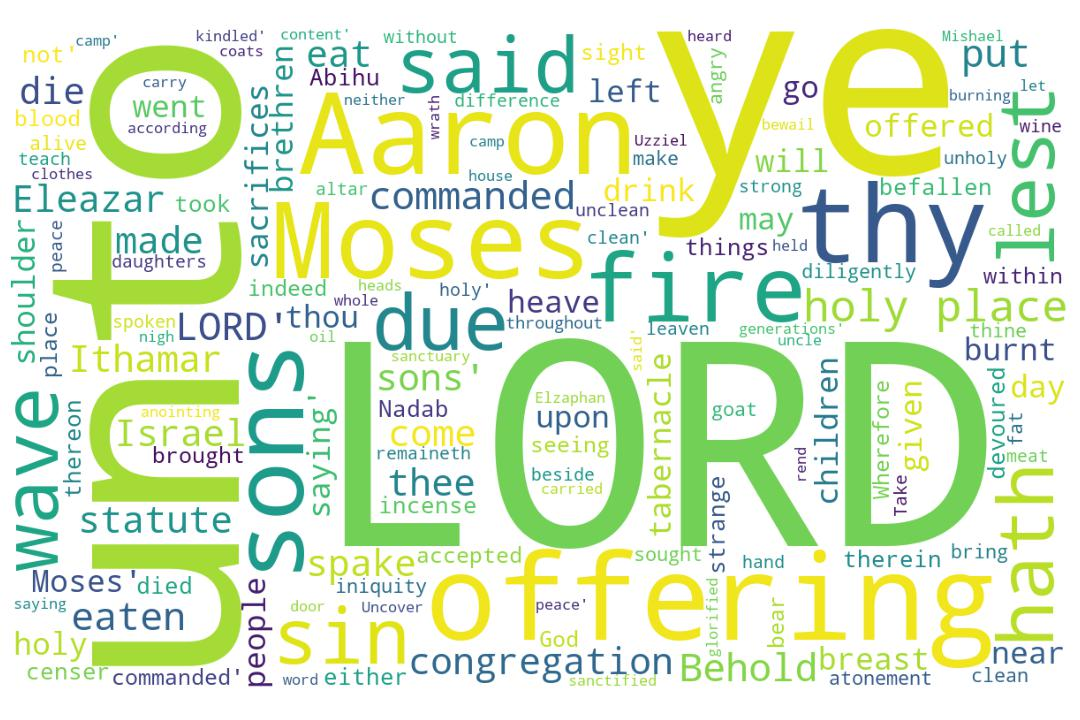
\includegraphics[width=\linewidth]{03OT-Leviticus/Leviticus10-WordCloud.jpg}
  \caption{Leviticus 10 Word Cloud}
  \label{fig:Leviticus 10 word Cloud}
\end{figure}

\marginpar{\scriptsize \centering \fcolorbox{bone}{lime}{\textbf{STRANGE FIRE}}\\ (Leviticus 10:1--20) 
\begin{compactenum}[I.][8]
	\item The \textbf{Censers} \index[scripture]{Leviticus!Lev 10:01}(Lev 10:1)
	\item The \textbf{Corruption} \index[scripture]{Leviticus!Lev 10:02}(Lev 10:2)
	\item The \textbf{Consumption} \index[scripture]{Leviticus!Lev 10:02}(Lev 10:2)
	\item The \textbf{Corpses}  \index[scripture]{Leviticus!Lev 10:04}(Lev 10:4)
	\item The \textbf{Carrying} Away \index[scripture]{Leviticus!Lev 10:05}(Lev 10:5) cf \index[scripture]{Acts!Acts 05:09}(Acts 5:9)
	\item The \textbf{Congregation}  \index[scripture]{Leviticus!Lev 10:07}\index[scripture]{Leviticus!Lev 10:09}\index[scripture]{Leviticus!Lev 10:17}(Lev 10:7, 9, 17) (which undoubtedly sought an explanation)
	\item The \textbf{Correction}  \index[scripture]{Leviticus!Lev 10:09--10}(Lev 10:9--10) (establishing the distinction between holy and unholy)
\end{compactenum} }

%%%%%%%%%%%%%%%%%%%%%%%%%%%
%%%%%%%%%%%%%%%%%%%%%%%%%%%
\footnote{\textcolor[cmyk]{0.99998,1,0,0}{\hyperlink{TOC}{Return to end of Table of Contents.}}}\footnote{\href{https://audiobible.com/bible/leviticus_10.html}{\textcolor[cmyk]{0.99998,1,0,0}{Leviticus 10 Audio}}}\textcolor[cmyk]{0.99998,1,0,0}{And Nadab and Abihu, the sons of Aaron, took either of them his \fcolorbox{bone}{lime}{censer}, and put fire therein, and put incense thereon, and offered strange fire before the LORD, which he commanded them not.}
[2] \textcolor[cmyk]{0.99998,1,0,0}{And there went out fire from the LORD, and \fcolorbox{bone}{lime}{devoured} them, and \fcolorbox{bone}{lime}{they died} before the LORD.}
[3] \textcolor[cmyk]{0.99998,1,0,0}{Then Moses said unto Aaron, This \emph{is} \emph{it} that the LORD spake, saying, I will be sanctified in them that come nigh me, and before all the people I will be glorified. And Aaron held his peace.}
[4] \textcolor[cmyk]{0.99998,1,0,0}{And Moses called Mishael and Elzaphan, the sons of Uzziel the uncle of Aaron, and said unto them, Come near, \fcolorbox{bone}{lime}{carry your brethren} from before the sanctuary out of the camp.}
[5] \textcolor[cmyk]{0.99998,1,0,0}{So they went near, and \fcolorbox{bone}{lime}{carried} them in their coats out of the camp; as Moses had said.}
[6] \textcolor[cmyk]{0.99998,1,0,0}{And Moses said unto Aaron, and unto Eleazar and unto Ithamar, his sons, Uncover not your heads, neither rend your clothes; lest ye die, and lest wrath come upon all the people: but let your brethren, the whole house of Israel, bewail the burning which the LORD hath kindled.}
[7] \textcolor[cmyk]{0.99998,1,0,0}{And ye shall not go out from the door of the tabernacle of the \fcolorbox{bone}{lime}{congregation}, lest ye die: for the anointing oil of the LORD \emph{is} upon you. And they did according to the word of Moses.}\\
\\
\P \textcolor[cmyk]{0.99998,1,0,0}{And the LORD spake unto Aaron, saying,}
[9] \textcolor[cmyk]{0.99998,1,0,0}{Do not drink wine nor strong drink, thou, nor thy sons with thee, when ye go into the tabernacle of the congregation, lest ye die: \emph{it} \emph{shall} \emph{be} a statute for ever throughout your generations:}
[10] \textcolor[cmyk]{0.99998,1,0,0}{And that ye may put \fcolorbox{bone}{lime}{difference} between holy and unholy, and between unclean and clean;}
[11] \textcolor[cmyk]{0.99998,1,0,0}{And that ye may teach the children of Israel all the statutes which the LORD hath spoken unto them by the hand of Moses.}\\
\\
\P \textcolor[cmyk]{0.99998,1,0,0}{And Moses spake unto Aaron, and unto Eleazar and unto Ithamar, his sons that were left, Take the meat offering that remaineth of the offerings of the LORD made by fire, and eat it without leaven beside the altar: for it \emph{is} most holy:}
[13] \textcolor[cmyk]{0.99998,1,0,0}{And ye shall eat it in the holy place, because it \emph{is} thy due, and thy sons' due, of the sacrifices of the LORD made by fire: for so I am commanded.}
[14] \textcolor[cmyk]{0.99998,1,0,0}{And the wave breast and heave shoulder shall ye eat in a clean place; thou, and thy sons, and thy daughters with thee: for \emph{they} \emph{be} thy due, and thy sons' due, \emph{which} are given out of the sacrifices of peace offerings of the children of Israel.}
[15] \textcolor[cmyk]{0.99998,1,0,0}{The heave shoulder and the wave breast shall they bring with the offerings made by fire of the fat, to wave \emph{it} \emph{for} a wave offering before the LORD; and it shall be thine, and thy sons' with thee, by a statute for ever; as the LORD hath commanded.}\\
\\
\P \textcolor[cmyk]{0.99998,1,0,0}{And Moses diligently sought the goat of the sin offering, and, behold, it was burnt: and he was angry with Eleazar and Ithamar, the sons of Aaron \emph{which} \emph{were} left \emph{alive}, saying,}
[17] \textcolor[cmyk]{0.99998,1,0,0}{Wherefore have ye not eaten the sin offering in the holy place, seeing it \emph{is} most holy, and \emph{God} hath given it you to bear the iniquity of the congregation, to make atonement for them before the LORD?}
[18] \textcolor[cmyk]{0.99998,1,0,0}{Behold, the blood of it was not brought in within the holy \emph{place}: ye should indeed have eaten it in the holy \emph{place}, as I commanded.}
[19] \textcolor[cmyk]{0.99998,1,0,0}{And Aaron said unto Moses, Behold, this day have they offered their sin offering and their burnt offering before the LORD; and such things have befallen me: and \emph{if} I had eaten the sin offering to day, should it have been accepted in the sight of the LORD?}
[20] \textcolor[cmyk]{0.99998,1,0,0}{And when Moses heard \emph{that}, he was content.}
\index[NWIV]{34!Leviticus!Lev 10:1}\index[AWIP]{And!Leviticus!Lev 10:1}\index[AWIP]{Nadab!Leviticus!Lev 10:1}\index[AWIP]{and!Leviticus!Lev 10:1}\index[AWIP]{and!Leviticus!Lev 10:1 (2)}\index[AWIP]{and!Leviticus!Lev 10:1 (3)}\index[AWIP]{and!Leviticus!Lev 10:1 (4)}\index[AWIP]{Abihu!Leviticus!Lev 10:1}\index[AWIP]{the!Leviticus!Lev 10:1}\index[AWIP]{the!Leviticus!Lev 10:1 (2)}\index[AWIP]{sons!Leviticus!Lev 10:1}\index[AWIP]{of!Leviticus!Lev 10:1}\index[AWIP]{of!Leviticus!Lev 10:1 (2)}\index[AWIP]{Aaron!Leviticus!Lev 10:1}\index[AWIP]{took!Leviticus!Lev 10:1}\index[AWIP]{either!Leviticus!Lev 10:1}\index[AWIP]{them!Leviticus!Lev 10:1}\index[AWIP]{them!Leviticus!Lev 10:1 (2)}\index[AWIP]{his!Leviticus!Lev 10:1}\index[AWIP]{censer!Leviticus!Lev 10:1}\index[AWIP]{put!Leviticus!Lev 10:1}\index[AWIP]{put!Leviticus!Lev 10:1 (2)}\index[AWIP]{fire!Leviticus!Lev 10:1}\index[AWIP]{fire!Leviticus!Lev 10:1 (2)}\index[AWIP]{therein!Leviticus!Lev 10:1}\index[AWIP]{incense!Leviticus!Lev 10:1}\index[AWIP]{thereon!Leviticus!Lev 10:1}\index[AWIP]{offered!Leviticus!Lev 10:1}\index[AWIP]{strange!Leviticus!Lev 10:1}\index[AWIP]{before!Leviticus!Lev 10:1}\index[AWIP]{LORD!Leviticus!Lev 10:1}\index[AWIP]{which!Leviticus!Lev 10:1}\index[AWIP]{he!Leviticus!Lev 10:1}\index[AWIP]{commanded!Leviticus!Lev 10:1}\index[AWIP]{not!Leviticus!Lev 10:1}

\index[NWIV]{17!Leviticus!Lev 10:2}\index[AWIP]{And!Leviticus!Lev 10:2}\index[AWIP]{there!Leviticus!Lev 10:2}\index[AWIP]{went!Leviticus!Lev 10:2}\index[AWIP]{out!Leviticus!Lev 10:2}\index[AWIP]{fire!Leviticus!Lev 10:2}\index[AWIP]{from!Leviticus!Lev 10:2}\index[AWIP]{the!Leviticus!Lev 10:2}\index[AWIP]{the!Leviticus!Lev 10:2 (2)}\index[AWIP]{LORD!Leviticus!Lev 10:2}\index[AWIP]{LORD!Leviticus!Lev 10:2 (2)}\index[AWIP]{and!Leviticus!Lev 10:2}\index[AWIP]{and!Leviticus!Lev 10:2 (2)}\index[AWIP]{devoured!Leviticus!Lev 10:2}\index[AWIP]{them!Leviticus!Lev 10:2}\index[AWIP]{they!Leviticus!Lev 10:2}\index[AWIP]{died!Leviticus!Lev 10:2}\index[AWIP]{before!Leviticus!Lev 10:2}

\index[NWIV]{37!Leviticus!Lev 10:3}\index[AWIP]{Then!Leviticus!Lev 10:3}\index[AWIP]{Moses!Leviticus!Lev 10:3}\index[AWIP]{said!Leviticus!Lev 10:3}\index[AWIP]{unto!Leviticus!Lev 10:3}\index[AWIP]{Aaron!Leviticus!Lev 10:3}\index[AWIP]{Aaron!Leviticus!Lev 10:3 (2)}\index[AWIP]{This!Leviticus!Lev 10:3}\index[AWIP]{\emph{is}!Leviticus!Lev 10:3}\index[AWIP]{\emph{it}!Leviticus!Lev 10:3}\index[AWIP]{that!Leviticus!Lev 10:3}\index[AWIP]{that!Leviticus!Lev 10:3 (2)}\index[AWIP]{the!Leviticus!Lev 10:3}\index[AWIP]{the!Leviticus!Lev 10:3 (2)}\index[AWIP]{LORD!Leviticus!Lev 10:3}\index[AWIP]{spake!Leviticus!Lev 10:3}\index[AWIP]{saying!Leviticus!Lev 10:3}\index[AWIP]{I!Leviticus!Lev 10:3}\index[AWIP]{I!Leviticus!Lev 10:3 (2)}\index[AWIP]{will!Leviticus!Lev 10:3}\index[AWIP]{will!Leviticus!Lev 10:3 (2)}\index[AWIP]{be!Leviticus!Lev 10:3}\index[AWIP]{be!Leviticus!Lev 10:3 (2)}\index[AWIP]{sanctified!Leviticus!Lev 10:3}\index[AWIP]{in!Leviticus!Lev 10:3}\index[AWIP]{them!Leviticus!Lev 10:3}\index[AWIP]{come!Leviticus!Lev 10:3}\index[AWIP]{nigh!Leviticus!Lev 10:3}\index[AWIP]{me!Leviticus!Lev 10:3}\index[AWIP]{and!Leviticus!Lev 10:3}\index[AWIP]{before!Leviticus!Lev 10:3}\index[AWIP]{all!Leviticus!Lev 10:3}\index[AWIP]{people!Leviticus!Lev 10:3}\index[AWIP]{glorified!Leviticus!Lev 10:3}\index[AWIP]{And!Leviticus!Lev 10:3}\index[AWIP]{held!Leviticus!Lev 10:3}\index[AWIP]{his!Leviticus!Lev 10:3}\index[AWIP]{peace!Leviticus!Lev 10:3}\index[AWIP]{\emph{is}!Leviticus!Lev 10:3}\index[AWIP]{\emph{it}!Leviticus!Lev 10:3}

\index[NWIV]{31!Leviticus!Lev 10:4}\index[AWIP]{And!Leviticus!Lev 10:4}\index[AWIP]{Moses!Leviticus!Lev 10:4}\index[AWIP]{called!Leviticus!Lev 10:4}\index[AWIP]{Mishael!Leviticus!Lev 10:4}\index[AWIP]{and!Leviticus!Lev 10:4}\index[AWIP]{and!Leviticus!Lev 10:4 (2)}\index[AWIP]{Elzaphan!Leviticus!Lev 10:4}\index[AWIP]{the!Leviticus!Lev 10:4}\index[AWIP]{the!Leviticus!Lev 10:4 (2)}\index[AWIP]{the!Leviticus!Lev 10:4 (3)}\index[AWIP]{the!Leviticus!Lev 10:4 (4)}\index[AWIP]{sons!Leviticus!Lev 10:4}\index[AWIP]{of!Leviticus!Lev 10:4}\index[AWIP]{of!Leviticus!Lev 10:4 (2)}\index[AWIP]{of!Leviticus!Lev 10:4 (3)}\index[AWIP]{Uzziel!Leviticus!Lev 10:4}\index[AWIP]{uncle!Leviticus!Lev 10:4}\index[AWIP]{Aaron!Leviticus!Lev 10:4}\index[AWIP]{said!Leviticus!Lev 10:4}\index[AWIP]{unto!Leviticus!Lev 10:4}\index[AWIP]{them!Leviticus!Lev 10:4}\index[AWIP]{Come!Leviticus!Lev 10:4}\index[AWIP]{near!Leviticus!Lev 10:4}\index[AWIP]{carry!Leviticus!Lev 10:4}\index[AWIP]{your!Leviticus!Lev 10:4}\index[AWIP]{brethren!Leviticus!Lev 10:4}\index[AWIP]{from!Leviticus!Lev 10:4}\index[AWIP]{before!Leviticus!Lev 10:4}\index[AWIP]{sanctuary!Leviticus!Lev 10:4}\index[AWIP]{out!Leviticus!Lev 10:4}\index[AWIP]{camp!Leviticus!Lev 10:4}

\index[NWIV]{18!Leviticus!Lev 10:5}\index[AWIP]{So!Leviticus!Lev 10:5}\index[AWIP]{they!Leviticus!Lev 10:5}\index[AWIP]{went!Leviticus!Lev 10:5}\index[AWIP]{near!Leviticus!Lev 10:5}\index[AWIP]{and!Leviticus!Lev 10:5}\index[AWIP]{carried!Leviticus!Lev 10:5}\index[AWIP]{them!Leviticus!Lev 10:5}\index[AWIP]{in!Leviticus!Lev 10:5}\index[AWIP]{their!Leviticus!Lev 10:5}\index[AWIP]{coats!Leviticus!Lev 10:5}\index[AWIP]{out!Leviticus!Lev 10:5}\index[AWIP]{of!Leviticus!Lev 10:5}\index[AWIP]{the!Leviticus!Lev 10:5}\index[AWIP]{camp!Leviticus!Lev 10:5}\index[AWIP]{as!Leviticus!Lev 10:5}\index[AWIP]{Moses!Leviticus!Lev 10:5}\index[AWIP]{had!Leviticus!Lev 10:5}\index[AWIP]{said!Leviticus!Lev 10:5}

\index[NWIV]{49!Leviticus!Lev 10:6}\index[AWIP]{And!Leviticus!Lev 10:6}\index[AWIP]{Moses!Leviticus!Lev 10:6}\index[AWIP]{said!Leviticus!Lev 10:6}\index[AWIP]{unto!Leviticus!Lev 10:6}\index[AWIP]{unto!Leviticus!Lev 10:6 (2)}\index[AWIP]{unto!Leviticus!Lev 10:6 (3)}\index[AWIP]{Aaron!Leviticus!Lev 10:6}\index[AWIP]{and!Leviticus!Lev 10:6}\index[AWIP]{and!Leviticus!Lev 10:6 (2)}\index[AWIP]{and!Leviticus!Lev 10:6 (3)}\index[AWIP]{Eleazar!Leviticus!Lev 10:6}\index[AWIP]{Ithamar!Leviticus!Lev 10:6}\index[AWIP]{his!Leviticus!Lev 10:6}\index[AWIP]{sons!Leviticus!Lev 10:6}\index[AWIP]{Uncover!Leviticus!Lev 10:6}\index[AWIP]{not!Leviticus!Lev 10:6}\index[AWIP]{your!Leviticus!Lev 10:6}\index[AWIP]{your!Leviticus!Lev 10:6 (2)}\index[AWIP]{your!Leviticus!Lev 10:6 (3)}\index[AWIP]{heads!Leviticus!Lev 10:6}\index[AWIP]{neither!Leviticus!Lev 10:6}\index[AWIP]{rend!Leviticus!Lev 10:6}\index[AWIP]{clothes!Leviticus!Lev 10:6}\index[AWIP]{lest!Leviticus!Lev 10:6}\index[AWIP]{lest!Leviticus!Lev 10:6 (2)}\index[AWIP]{ye!Leviticus!Lev 10:6}\index[AWIP]{die!Leviticus!Lev 10:6}\index[AWIP]{wrath!Leviticus!Lev 10:6}\index[AWIP]{come!Leviticus!Lev 10:6}\index[AWIP]{upon!Leviticus!Lev 10:6}\index[AWIP]{all!Leviticus!Lev 10:6}\index[AWIP]{the!Leviticus!Lev 10:6}\index[AWIP]{the!Leviticus!Lev 10:6 (2)}\index[AWIP]{the!Leviticus!Lev 10:6 (3)}\index[AWIP]{the!Leviticus!Lev 10:6 (4)}\index[AWIP]{people!Leviticus!Lev 10:6}\index[AWIP]{but!Leviticus!Lev 10:6}\index[AWIP]{let!Leviticus!Lev 10:6}\index[AWIP]{brethren!Leviticus!Lev 10:6}\index[AWIP]{whole!Leviticus!Lev 10:6}\index[AWIP]{house!Leviticus!Lev 10:6}\index[AWIP]{of!Leviticus!Lev 10:6}\index[AWIP]{Israel!Leviticus!Lev 10:6}\index[AWIP]{bewail!Leviticus!Lev 10:6}\index[AWIP]{burning!Leviticus!Lev 10:6}\index[AWIP]{which!Leviticus!Lev 10:6}\index[AWIP]{LORD!Leviticus!Lev 10:6}\index[AWIP]{hath!Leviticus!Lev 10:6}\index[AWIP]{kindled!Leviticus!Lev 10:6}

\index[NWIV]{37!Leviticus!Lev 10:7}\index[AWIP]{And!Leviticus!Lev 10:7}\index[AWIP]{And!Leviticus!Lev 10:7 (2)}\index[AWIP]{ye!Leviticus!Lev 10:7}\index[AWIP]{ye!Leviticus!Lev 10:7 (2)}\index[AWIP]{shall!Leviticus!Lev 10:7}\index[AWIP]{not!Leviticus!Lev 10:7}\index[AWIP]{go!Leviticus!Lev 10:7}\index[AWIP]{out!Leviticus!Lev 10:7}\index[AWIP]{from!Leviticus!Lev 10:7}\index[AWIP]{the!Leviticus!Lev 10:7}\index[AWIP]{the!Leviticus!Lev 10:7 (2)}\index[AWIP]{the!Leviticus!Lev 10:7 (3)}\index[AWIP]{the!Leviticus!Lev 10:7 (4)}\index[AWIP]{the!Leviticus!Lev 10:7 (5)}\index[AWIP]{the!Leviticus!Lev 10:7 (6)}\index[AWIP]{door!Leviticus!Lev 10:7}\index[AWIP]{of!Leviticus!Lev 10:7}\index[AWIP]{of!Leviticus!Lev 10:7 (2)}\index[AWIP]{of!Leviticus!Lev 10:7 (3)}\index[AWIP]{of!Leviticus!Lev 10:7 (4)}\index[AWIP]{tabernacle!Leviticus!Lev 10:7}\index[AWIP]{congregation!Leviticus!Lev 10:7}\index[AWIP]{lest!Leviticus!Lev 10:7}\index[AWIP]{die!Leviticus!Lev 10:7}\index[AWIP]{for!Leviticus!Lev 10:7}\index[AWIP]{anointing!Leviticus!Lev 10:7}\index[AWIP]{oil!Leviticus!Lev 10:7}\index[AWIP]{LORD!Leviticus!Lev 10:7}\index[AWIP]{\emph{is}!Leviticus!Lev 10:7}\index[AWIP]{upon!Leviticus!Lev 10:7}\index[AWIP]{you!Leviticus!Lev 10:7}\index[AWIP]{they!Leviticus!Lev 10:7}\index[AWIP]{did!Leviticus!Lev 10:7}\index[AWIP]{according!Leviticus!Lev 10:7}\index[AWIP]{to!Leviticus!Lev 10:7}\index[AWIP]{word!Leviticus!Lev 10:7}\index[AWIP]{Moses!Leviticus!Lev 10:7}\index[AWIP]{\emph{is}!Leviticus!Lev 10:7}

\index[NWIV]{7!Leviticus!Lev 10:8}\index[AWIP]{And!Leviticus!Lev 10:8}\index[AWIP]{the!Leviticus!Lev 10:8}\index[AWIP]{LORD!Leviticus!Lev 10:8}\index[AWIP]{spake!Leviticus!Lev 10:8}\index[AWIP]{unto!Leviticus!Lev 10:8}\index[AWIP]{Aaron!Leviticus!Lev 10:8}\index[AWIP]{saying!Leviticus!Lev 10:8}

\index[NWIV]{35!Leviticus!Lev 10:9}\index[AWIP]{Do!Leviticus!Lev 10:9}\index[AWIP]{not!Leviticus!Lev 10:9}\index[AWIP]{drink!Leviticus!Lev 10:9}\index[AWIP]{drink!Leviticus!Lev 10:9 (2)}\index[AWIP]{wine!Leviticus!Lev 10:9}\index[AWIP]{nor!Leviticus!Lev 10:9}\index[AWIP]{nor!Leviticus!Lev 10:9 (2)}\index[AWIP]{strong!Leviticus!Lev 10:9}\index[AWIP]{thou!Leviticus!Lev 10:9}\index[AWIP]{thy!Leviticus!Lev 10:9}\index[AWIP]{sons!Leviticus!Lev 10:9}\index[AWIP]{with!Leviticus!Lev 10:9}\index[AWIP]{thee!Leviticus!Lev 10:9}\index[AWIP]{when!Leviticus!Lev 10:9}\index[AWIP]{ye!Leviticus!Lev 10:9}\index[AWIP]{ye!Leviticus!Lev 10:9 (2)}\index[AWIP]{go!Leviticus!Lev 10:9}\index[AWIP]{into!Leviticus!Lev 10:9}\index[AWIP]{the!Leviticus!Lev 10:9}\index[AWIP]{the!Leviticus!Lev 10:9 (2)}\index[AWIP]{tabernacle!Leviticus!Lev 10:9}\index[AWIP]{of!Leviticus!Lev 10:9}\index[AWIP]{congregation!Leviticus!Lev 10:9}\index[AWIP]{lest!Leviticus!Lev 10:9}\index[AWIP]{die!Leviticus!Lev 10:9}\index[AWIP]{\emph{it}!Leviticus!Lev 10:9}\index[AWIP]{\emph{shall}!Leviticus!Lev 10:9}\index[AWIP]{\emph{be}!Leviticus!Lev 10:9}\index[AWIP]{a!Leviticus!Lev 10:9}\index[AWIP]{statute!Leviticus!Lev 10:9}\index[AWIP]{for!Leviticus!Lev 10:9}\index[AWIP]{ever!Leviticus!Lev 10:9}\index[AWIP]{throughout!Leviticus!Lev 10:9}\index[AWIP]{your!Leviticus!Lev 10:9}\index[AWIP]{generations!Leviticus!Lev 10:9}\index[AWIP]{\emph{it}!Leviticus!Lev 10:9}\index[AWIP]{\emph{shall}!Leviticus!Lev 10:9}\index[AWIP]{\emph{be}!Leviticus!Lev 10:9}

\index[NWIV]{15!Leviticus!Lev 10:10}\index[AWIP]{And!Leviticus!Lev 10:10}\index[AWIP]{that!Leviticus!Lev 10:10}\index[AWIP]{ye!Leviticus!Lev 10:10}\index[AWIP]{may!Leviticus!Lev 10:10}\index[AWIP]{put!Leviticus!Lev 10:10}\index[AWIP]{difference!Leviticus!Lev 10:10}\index[AWIP]{between!Leviticus!Lev 10:10}\index[AWIP]{between!Leviticus!Lev 10:10 (2)}\index[AWIP]{holy!Leviticus!Lev 10:10}\index[AWIP]{and!Leviticus!Lev 10:10}\index[AWIP]{and!Leviticus!Lev 10:10 (2)}\index[AWIP]{and!Leviticus!Lev 10:10 (3)}\index[AWIP]{unholy!Leviticus!Lev 10:10}\index[AWIP]{unclean!Leviticus!Lev 10:10}\index[AWIP]{clean!Leviticus!Lev 10:10}

\index[NWIV]{24!Leviticus!Lev 10:11}\index[AWIP]{And!Leviticus!Lev 10:11}\index[AWIP]{that!Leviticus!Lev 10:11}\index[AWIP]{ye!Leviticus!Lev 10:11}\index[AWIP]{may!Leviticus!Lev 10:11}\index[AWIP]{teach!Leviticus!Lev 10:11}\index[AWIP]{the!Leviticus!Lev 10:11}\index[AWIP]{the!Leviticus!Lev 10:11 (2)}\index[AWIP]{the!Leviticus!Lev 10:11 (3)}\index[AWIP]{the!Leviticus!Lev 10:11 (4)}\index[AWIP]{children!Leviticus!Lev 10:11}\index[AWIP]{of!Leviticus!Lev 10:11}\index[AWIP]{of!Leviticus!Lev 10:11 (2)}\index[AWIP]{Israel!Leviticus!Lev 10:11}\index[AWIP]{all!Leviticus!Lev 10:11}\index[AWIP]{statutes!Leviticus!Lev 10:11}\index[AWIP]{which!Leviticus!Lev 10:11}\index[AWIP]{LORD!Leviticus!Lev 10:11}\index[AWIP]{hath!Leviticus!Lev 10:11}\index[AWIP]{spoken!Leviticus!Lev 10:11}\index[AWIP]{unto!Leviticus!Lev 10:11}\index[AWIP]{them!Leviticus!Lev 10:11}\index[AWIP]{by!Leviticus!Lev 10:11}\index[AWIP]{hand!Leviticus!Lev 10:11}\index[AWIP]{Moses!Leviticus!Lev 10:11}

\index[NWIV]{44!Leviticus!Lev 10:12}\index[AWIP]{And!Leviticus!Lev 10:12}\index[AWIP]{Moses!Leviticus!Lev 10:12}\index[AWIP]{spake!Leviticus!Lev 10:12}\index[AWIP]{unto!Leviticus!Lev 10:12}\index[AWIP]{unto!Leviticus!Lev 10:12 (2)}\index[AWIP]{unto!Leviticus!Lev 10:12 (3)}\index[AWIP]{Aaron!Leviticus!Lev 10:12}\index[AWIP]{and!Leviticus!Lev 10:12}\index[AWIP]{and!Leviticus!Lev 10:12 (2)}\index[AWIP]{and!Leviticus!Lev 10:12 (3)}\index[AWIP]{Eleazar!Leviticus!Lev 10:12}\index[AWIP]{Ithamar!Leviticus!Lev 10:12}\index[AWIP]{his!Leviticus!Lev 10:12}\index[AWIP]{sons!Leviticus!Lev 10:12}\index[AWIP]{that!Leviticus!Lev 10:12}\index[AWIP]{that!Leviticus!Lev 10:12 (2)}\index[AWIP]{were!Leviticus!Lev 10:12}\index[AWIP]{left!Leviticus!Lev 10:12}\index[AWIP]{Take!Leviticus!Lev 10:12}\index[AWIP]{the!Leviticus!Lev 10:12}\index[AWIP]{the!Leviticus!Lev 10:12 (2)}\index[AWIP]{the!Leviticus!Lev 10:12 (3)}\index[AWIP]{the!Leviticus!Lev 10:12 (4)}\index[AWIP]{meat!Leviticus!Lev 10:12}\index[AWIP]{offering!Leviticus!Lev 10:12}\index[AWIP]{remaineth!Leviticus!Lev 10:12}\index[AWIP]{of!Leviticus!Lev 10:12}\index[AWIP]{of!Leviticus!Lev 10:12 (2)}\index[AWIP]{offerings!Leviticus!Lev 10:12}\index[AWIP]{LORD!Leviticus!Lev 10:12}\index[AWIP]{made!Leviticus!Lev 10:12}\index[AWIP]{by!Leviticus!Lev 10:12}\index[AWIP]{fire!Leviticus!Lev 10:12}\index[AWIP]{eat!Leviticus!Lev 10:12}\index[AWIP]{it!Leviticus!Lev 10:12}\index[AWIP]{it!Leviticus!Lev 10:12 (2)}\index[AWIP]{without!Leviticus!Lev 10:12}\index[AWIP]{leaven!Leviticus!Lev 10:12}\index[AWIP]{beside!Leviticus!Lev 10:12}\index[AWIP]{altar!Leviticus!Lev 10:12}\index[AWIP]{for!Leviticus!Lev 10:12}\index[AWIP]{\emph{is}!Leviticus!Lev 10:12}\index[AWIP]{most!Leviticus!Lev 10:12}\index[AWIP]{holy!Leviticus!Lev 10:12}\index[AWIP]{\emph{is}!Leviticus!Lev 10:12}

\index[NWIV]{32!Leviticus!Lev 10:13}\index[AWIP]{And!Leviticus!Lev 10:13}\index[AWIP]{ye!Leviticus!Lev 10:13}\index[AWIP]{shall!Leviticus!Lev 10:13}\index[AWIP]{eat!Leviticus!Lev 10:13}\index[AWIP]{it!Leviticus!Lev 10:13}\index[AWIP]{it!Leviticus!Lev 10:13 (2)}\index[AWIP]{in!Leviticus!Lev 10:13}\index[AWIP]{the!Leviticus!Lev 10:13}\index[AWIP]{the!Leviticus!Lev 10:13 (2)}\index[AWIP]{the!Leviticus!Lev 10:13 (3)}\index[AWIP]{holy!Leviticus!Lev 10:13}\index[AWIP]{place!Leviticus!Lev 10:13}\index[AWIP]{because!Leviticus!Lev 10:13}\index[AWIP]{\emph{is}!Leviticus!Lev 10:13}\index[AWIP]{thy!Leviticus!Lev 10:13}\index[AWIP]{thy!Leviticus!Lev 10:13 (2)}\index[AWIP]{due!Leviticus!Lev 10:13}\index[AWIP]{due!Leviticus!Lev 10:13 (2)}\index[AWIP]{and!Leviticus!Lev 10:13}\index[AWIP]{sons'!Leviticus!Lev 10:13}\index[AWIP]{of!Leviticus!Lev 10:13}\index[AWIP]{of!Leviticus!Lev 10:13 (2)}\index[AWIP]{sacrifices!Leviticus!Lev 10:13}\index[AWIP]{LORD!Leviticus!Lev 10:13}\index[AWIP]{made!Leviticus!Lev 10:13}\index[AWIP]{by!Leviticus!Lev 10:13}\index[AWIP]{fire!Leviticus!Lev 10:13}\index[AWIP]{for!Leviticus!Lev 10:13}\index[AWIP]{so!Leviticus!Lev 10:13}\index[AWIP]{I!Leviticus!Lev 10:13}\index[AWIP]{am!Leviticus!Lev 10:13}\index[AWIP]{commanded!Leviticus!Lev 10:13}\index[AWIP]{\emph{is}!Leviticus!Lev 10:13}

\index[NWIV]{47!Leviticus!Lev 10:14}\index[AWIP]{And!Leviticus!Lev 10:14}\index[AWIP]{the!Leviticus!Lev 10:14}\index[AWIP]{the!Leviticus!Lev 10:14 (2)}\index[AWIP]{the!Leviticus!Lev 10:14 (3)}\index[AWIP]{wave!Leviticus!Lev 10:14}\index[AWIP]{breast!Leviticus!Lev 10:14}\index[AWIP]{and!Leviticus!Lev 10:14}\index[AWIP]{and!Leviticus!Lev 10:14 (2)}\index[AWIP]{and!Leviticus!Lev 10:14 (3)}\index[AWIP]{and!Leviticus!Lev 10:14 (4)}\index[AWIP]{heave!Leviticus!Lev 10:14}\index[AWIP]{shoulder!Leviticus!Lev 10:14}\index[AWIP]{shall!Leviticus!Lev 10:14}\index[AWIP]{ye!Leviticus!Lev 10:14}\index[AWIP]{eat!Leviticus!Lev 10:14}\index[AWIP]{in!Leviticus!Lev 10:14}\index[AWIP]{a!Leviticus!Lev 10:14}\index[AWIP]{clean!Leviticus!Lev 10:14}\index[AWIP]{place!Leviticus!Lev 10:14}\index[AWIP]{thou!Leviticus!Lev 10:14}\index[AWIP]{thy!Leviticus!Lev 10:14}\index[AWIP]{thy!Leviticus!Lev 10:14 (2)}\index[AWIP]{thy!Leviticus!Lev 10:14 (3)}\index[AWIP]{thy!Leviticus!Lev 10:14 (4)}\index[AWIP]{sons!Leviticus!Lev 10:14}\index[AWIP]{daughters!Leviticus!Lev 10:14}\index[AWIP]{with!Leviticus!Lev 10:14}\index[AWIP]{thee!Leviticus!Lev 10:14}\index[AWIP]{for!Leviticus!Lev 10:14}\index[AWIP]{\emph{they}!Leviticus!Lev 10:14}\index[AWIP]{\emph{be}!Leviticus!Lev 10:14}\index[AWIP]{due!Leviticus!Lev 10:14}\index[AWIP]{due!Leviticus!Lev 10:14 (2)}\index[AWIP]{sons'!Leviticus!Lev 10:14}\index[AWIP]{\emph{which}!Leviticus!Lev 10:14}\index[AWIP]{are!Leviticus!Lev 10:14}\index[AWIP]{given!Leviticus!Lev 10:14}\index[AWIP]{out!Leviticus!Lev 10:14}\index[AWIP]{of!Leviticus!Lev 10:14}\index[AWIP]{of!Leviticus!Lev 10:14 (2)}\index[AWIP]{of!Leviticus!Lev 10:14 (3)}\index[AWIP]{of!Leviticus!Lev 10:14 (4)}\index[AWIP]{sacrifices!Leviticus!Lev 10:14}\index[AWIP]{peace!Leviticus!Lev 10:14}\index[AWIP]{offerings!Leviticus!Lev 10:14}\index[AWIP]{children!Leviticus!Lev 10:14}\index[AWIP]{Israel!Leviticus!Lev 10:14}\index[AWIP]{\emph{they}!Leviticus!Lev 10:14}\index[AWIP]{\emph{be}!Leviticus!Lev 10:14}\index[AWIP]{\emph{which}!Leviticus!Lev 10:14}

\index[NWIV]{49!Leviticus!Lev 10:15}\index[AWIP]{The!Leviticus!Lev 10:15}\index[AWIP]{heave!Leviticus!Lev 10:15}\index[AWIP]{shoulder!Leviticus!Lev 10:15}\index[AWIP]{and!Leviticus!Lev 10:15}\index[AWIP]{and!Leviticus!Lev 10:15 (2)}\index[AWIP]{and!Leviticus!Lev 10:15 (3)}\index[AWIP]{the!Leviticus!Lev 10:15}\index[AWIP]{the!Leviticus!Lev 10:15 (2)}\index[AWIP]{the!Leviticus!Lev 10:15 (3)}\index[AWIP]{the!Leviticus!Lev 10:15 (4)}\index[AWIP]{the!Leviticus!Lev 10:15 (5)}\index[AWIP]{wave!Leviticus!Lev 10:15}\index[AWIP]{wave!Leviticus!Lev 10:15 (2)}\index[AWIP]{wave!Leviticus!Lev 10:15 (3)}\index[AWIP]{breast!Leviticus!Lev 10:15}\index[AWIP]{shall!Leviticus!Lev 10:15}\index[AWIP]{shall!Leviticus!Lev 10:15 (2)}\index[AWIP]{they!Leviticus!Lev 10:15}\index[AWIP]{bring!Leviticus!Lev 10:15}\index[AWIP]{with!Leviticus!Lev 10:15}\index[AWIP]{with!Leviticus!Lev 10:15 (2)}\index[AWIP]{offerings!Leviticus!Lev 10:15}\index[AWIP]{made!Leviticus!Lev 10:15}\index[AWIP]{by!Leviticus!Lev 10:15}\index[AWIP]{by!Leviticus!Lev 10:15 (2)}\index[AWIP]{fire!Leviticus!Lev 10:15}\index[AWIP]{of!Leviticus!Lev 10:15}\index[AWIP]{fat!Leviticus!Lev 10:15}\index[AWIP]{to!Leviticus!Lev 10:15}\index[AWIP]{\emph{it}!Leviticus!Lev 10:15}\index[AWIP]{\emph{for}!Leviticus!Lev 10:15}\index[AWIP]{a!Leviticus!Lev 10:15}\index[AWIP]{a!Leviticus!Lev 10:15 (2)}\index[AWIP]{offering!Leviticus!Lev 10:15}\index[AWIP]{before!Leviticus!Lev 10:15}\index[AWIP]{LORD!Leviticus!Lev 10:15}\index[AWIP]{LORD!Leviticus!Lev 10:15 (2)}\index[AWIP]{it!Leviticus!Lev 10:15}\index[AWIP]{be!Leviticus!Lev 10:15}\index[AWIP]{thine!Leviticus!Lev 10:15}\index[AWIP]{thy!Leviticus!Lev 10:15}\index[AWIP]{sons'!Leviticus!Lev 10:15}\index[AWIP]{thee!Leviticus!Lev 10:15}\index[AWIP]{statute!Leviticus!Lev 10:15}\index[AWIP]{for!Leviticus!Lev 10:15}\index[AWIP]{ever!Leviticus!Lev 10:15}\index[AWIP]{as!Leviticus!Lev 10:15}\index[AWIP]{hath!Leviticus!Lev 10:15}\index[AWIP]{commanded!Leviticus!Lev 10:15}\index[AWIP]{\emph{it}!Leviticus!Lev 10:15}\index[AWIP]{\emph{for}!Leviticus!Lev 10:15}

\index[NWIV]{32!Leviticus!Lev 10:16}\index[AWIP]{And!Leviticus!Lev 10:16}\index[AWIP]{Moses!Leviticus!Lev 10:16}\index[AWIP]{diligently!Leviticus!Lev 10:16}\index[AWIP]{sought!Leviticus!Lev 10:16}\index[AWIP]{the!Leviticus!Lev 10:16}\index[AWIP]{the!Leviticus!Lev 10:16 (2)}\index[AWIP]{the!Leviticus!Lev 10:16 (3)}\index[AWIP]{goat!Leviticus!Lev 10:16}\index[AWIP]{of!Leviticus!Lev 10:16}\index[AWIP]{of!Leviticus!Lev 10:16 (2)}\index[AWIP]{sin!Leviticus!Lev 10:16}\index[AWIP]{offering!Leviticus!Lev 10:16}\index[AWIP]{and!Leviticus!Lev 10:16}\index[AWIP]{and!Leviticus!Lev 10:16 (2)}\index[AWIP]{and!Leviticus!Lev 10:16 (3)}\index[AWIP]{behold!Leviticus!Lev 10:16}\index[AWIP]{it!Leviticus!Lev 10:16}\index[AWIP]{was!Leviticus!Lev 10:16}\index[AWIP]{was!Leviticus!Lev 10:16 (2)}\index[AWIP]{burnt!Leviticus!Lev 10:16}\index[AWIP]{he!Leviticus!Lev 10:16}\index[AWIP]{angry!Leviticus!Lev 10:16}\index[AWIP]{with!Leviticus!Lev 10:16}\index[AWIP]{Eleazar!Leviticus!Lev 10:16}\index[AWIP]{Ithamar!Leviticus!Lev 10:16}\index[AWIP]{sons!Leviticus!Lev 10:16}\index[AWIP]{Aaron!Leviticus!Lev 10:16}\index[AWIP]{\emph{which}!Leviticus!Lev 10:16}\index[AWIP]{\emph{were}!Leviticus!Lev 10:16}\index[AWIP]{left!Leviticus!Lev 10:16}\index[AWIP]{\emph{alive}!Leviticus!Lev 10:16}\index[AWIP]{saying!Leviticus!Lev 10:16}\index[AWIP]{\emph{which}!Leviticus!Lev 10:16}\index[AWIP]{\emph{were}!Leviticus!Lev 10:16}\index[AWIP]{\emph{alive}!Leviticus!Lev 10:16}

\index[NWIV]{38!Leviticus!Lev 10:17}\index[AWIP]{Wherefore!Leviticus!Lev 10:17}\index[AWIP]{have!Leviticus!Lev 10:17}\index[AWIP]{ye!Leviticus!Lev 10:17}\index[AWIP]{not!Leviticus!Lev 10:17}\index[AWIP]{eaten!Leviticus!Lev 10:17}\index[AWIP]{the!Leviticus!Lev 10:17}\index[AWIP]{the!Leviticus!Lev 10:17 (2)}\index[AWIP]{the!Leviticus!Lev 10:17 (3)}\index[AWIP]{the!Leviticus!Lev 10:17 (4)}\index[AWIP]{the!Leviticus!Lev 10:17 (5)}\index[AWIP]{sin!Leviticus!Lev 10:17}\index[AWIP]{offering!Leviticus!Lev 10:17}\index[AWIP]{in!Leviticus!Lev 10:17}\index[AWIP]{holy!Leviticus!Lev 10:17}\index[AWIP]{holy!Leviticus!Lev 10:17 (2)}\index[AWIP]{place!Leviticus!Lev 10:17}\index[AWIP]{seeing!Leviticus!Lev 10:17}\index[AWIP]{it!Leviticus!Lev 10:17}\index[AWIP]{it!Leviticus!Lev 10:17 (2)}\index[AWIP]{\emph{is}!Leviticus!Lev 10:17}\index[AWIP]{most!Leviticus!Lev 10:17}\index[AWIP]{and!Leviticus!Lev 10:17}\index[AWIP]{\emph{God}!Leviticus!Lev 10:17}\index[AWIP]{hath!Leviticus!Lev 10:17}\index[AWIP]{given!Leviticus!Lev 10:17}\index[AWIP]{you!Leviticus!Lev 10:17}\index[AWIP]{to!Leviticus!Lev 10:17}\index[AWIP]{to!Leviticus!Lev 10:17 (2)}\index[AWIP]{bear!Leviticus!Lev 10:17}\index[AWIP]{iniquity!Leviticus!Lev 10:17}\index[AWIP]{of!Leviticus!Lev 10:17}\index[AWIP]{congregation!Leviticus!Lev 10:17}\index[AWIP]{make!Leviticus!Lev 10:17}\index[AWIP]{atonement!Leviticus!Lev 10:17}\index[AWIP]{for!Leviticus!Lev 10:17}\index[AWIP]{them!Leviticus!Lev 10:17}\index[AWIP]{before!Leviticus!Lev 10:17}\index[AWIP]{LORD?!Leviticus!Lev 10:17}\index[AWIP]{\emph{is}!Leviticus!Lev 10:17}\index[AWIP]{\emph{God}!Leviticus!Lev 10:17}

\index[NWIV]{26!Leviticus!Lev 10:18}\index[AWIP]{Behold!Leviticus!Lev 10:18}\index[AWIP]{the!Leviticus!Lev 10:18}\index[AWIP]{the!Leviticus!Lev 10:18 (2)}\index[AWIP]{the!Leviticus!Lev 10:18 (3)}\index[AWIP]{blood!Leviticus!Lev 10:18}\index[AWIP]{of!Leviticus!Lev 10:18}\index[AWIP]{it!Leviticus!Lev 10:18}\index[AWIP]{it!Leviticus!Lev 10:18 (2)}\index[AWIP]{was!Leviticus!Lev 10:18}\index[AWIP]{not!Leviticus!Lev 10:18}\index[AWIP]{brought!Leviticus!Lev 10:18}\index[AWIP]{in!Leviticus!Lev 10:18}\index[AWIP]{in!Leviticus!Lev 10:18 (2)}\index[AWIP]{within!Leviticus!Lev 10:18}\index[AWIP]{holy!Leviticus!Lev 10:18}\index[AWIP]{holy!Leviticus!Lev 10:18 (2)}\index[AWIP]{\emph{place}!Leviticus!Lev 10:18}\index[AWIP]{\emph{place}!Leviticus!Lev 10:18 (2)}\index[AWIP]{ye!Leviticus!Lev 10:18}\index[AWIP]{should!Leviticus!Lev 10:18}\index[AWIP]{indeed!Leviticus!Lev 10:18}\index[AWIP]{have!Leviticus!Lev 10:18}\index[AWIP]{eaten!Leviticus!Lev 10:18}\index[AWIP]{as!Leviticus!Lev 10:18}\index[AWIP]{I!Leviticus!Lev 10:18}\index[AWIP]{commanded!Leviticus!Lev 10:18}\index[AWIP]{\emph{place}!Leviticus!Lev 10:18}\index[AWIP]{\emph{place}!Leviticus!Lev 10:18 (2)}

\index[NWIV]{48!Leviticus!Lev 10:19}\index[AWIP]{And!Leviticus!Lev 10:19}\index[AWIP]{Aaron!Leviticus!Lev 10:19}\index[AWIP]{said!Leviticus!Lev 10:19}\index[AWIP]{unto!Leviticus!Lev 10:19}\index[AWIP]{Moses!Leviticus!Lev 10:19}\index[AWIP]{Behold!Leviticus!Lev 10:19}\index[AWIP]{this!Leviticus!Lev 10:19}\index[AWIP]{day!Leviticus!Lev 10:19}\index[AWIP]{day!Leviticus!Lev 10:19 (2)}\index[AWIP]{have!Leviticus!Lev 10:19}\index[AWIP]{have!Leviticus!Lev 10:19 (2)}\index[AWIP]{have!Leviticus!Lev 10:19 (3)}\index[AWIP]{they!Leviticus!Lev 10:19}\index[AWIP]{offered!Leviticus!Lev 10:19}\index[AWIP]{their!Leviticus!Lev 10:19}\index[AWIP]{their!Leviticus!Lev 10:19 (2)}\index[AWIP]{sin!Leviticus!Lev 10:19}\index[AWIP]{sin!Leviticus!Lev 10:19 (2)}\index[AWIP]{offering!Leviticus!Lev 10:19}\index[AWIP]{offering!Leviticus!Lev 10:19 (2)}\index[AWIP]{offering!Leviticus!Lev 10:19 (3)}\index[AWIP]{and!Leviticus!Lev 10:19}\index[AWIP]{and!Leviticus!Lev 10:19 (2)}\index[AWIP]{and!Leviticus!Lev 10:19 (3)}\index[AWIP]{burnt!Leviticus!Lev 10:19}\index[AWIP]{before!Leviticus!Lev 10:19}\index[AWIP]{the!Leviticus!Lev 10:19}\index[AWIP]{the!Leviticus!Lev 10:19 (2)}\index[AWIP]{the!Leviticus!Lev 10:19 (3)}\index[AWIP]{the!Leviticus!Lev 10:19 (4)}\index[AWIP]{LORD!Leviticus!Lev 10:19}\index[AWIP]{such!Leviticus!Lev 10:19}\index[AWIP]{things!Leviticus!Lev 10:19}\index[AWIP]{befallen!Leviticus!Lev 10:19}\index[AWIP]{me!Leviticus!Lev 10:19}\index[AWIP]{\emph{if}!Leviticus!Lev 10:19}\index[AWIP]{I!Leviticus!Lev 10:19}\index[AWIP]{had!Leviticus!Lev 10:19}\index[AWIP]{eaten!Leviticus!Lev 10:19}\index[AWIP]{to!Leviticus!Lev 10:19}\index[AWIP]{should!Leviticus!Lev 10:19}\index[AWIP]{it!Leviticus!Lev 10:19}\index[AWIP]{been!Leviticus!Lev 10:19}\index[AWIP]{accepted!Leviticus!Lev 10:19}\index[AWIP]{in!Leviticus!Lev 10:19}\index[AWIP]{sight!Leviticus!Lev 10:19}\index[AWIP]{of!Leviticus!Lev 10:19}\index[AWIP]{LORD?!Leviticus!Lev 10:19}\index[AWIP]{\emph{if}!Leviticus!Lev 10:19}

\index[NWIV]{8!Leviticus!Lev 10:20}\index[AWIP]{And!Leviticus!Lev 10:20}\index[AWIP]{when!Leviticus!Lev 10:20}\index[AWIP]{Moses!Leviticus!Lev 10:20}\index[AWIP]{heard!Leviticus!Lev 10:20}\index[AWIP]{\emph{that}!Leviticus!Lev 10:20}\index[AWIP]{he!Leviticus!Lev 10:20}\index[AWIP]{was!Leviticus!Lev 10:20}\index[AWIP]{content!Leviticus!Lev 10:20}\index[AWIP]{\emph{that}!Leviticus!Lev 10:20}


\section{Leviticus 10 Outlines}

\subsection{My Outlines}

\subsubsection{Strange Fire}
\index[speaker]{Keith Anthony!Leviticus 10 (Strange Fire)}
\index[series]{Leviticus (Keith Anthony)!Leviticus 10 (Strange Fire)}
\index[date]{2017/02/03!Leviticus 10 (Strange Fire) (Keith Anthony)}
\textbf{Introduction: }It has been suggested that the most serious crimes in Christianity have occurred and occur in the realm of corrupt worship.  We see it is Acts 5, where Ananias and Saphira were killed for lying  to the church.  We see it in Exodus 32 where a false image was worshiped as God. Here the exacting and precise requirements for worship are trivialized. So be careful what you call worship. Be careful what you think has to be manifested for something to be worship (and is not without). 
\begin{compactenum}[I.][7]
	\item The \textbf{Censers} \index[scripture]{Leviticus!Lev 10:01}(Lev 10:1)
	\item The \textbf{Corruption} \index[scripture]{Leviticus!Lev 10:02}(Lev 10:2)
	\item The \textbf{Consumption} \index[scripture]{Leviticus!Lev 10:02}(Lev 10:2)
	\item The \textbf{Corpses}  \index[scripture]{Leviticus!Lev 10:04}(Lev 10:4)
	\item The \textbf{Carrying} Away \index[scripture]{Leviticus!Lev 10:05}(Leviticus 10:5) cf \index[scripture]{Acts!Acts 05:09}(Acts 5:9)
	\item The \textbf{Congregation}  \index[scripture]{Leviticus!Lev 10:07}\index[scripture]{Leviticus!Lev 10:09}\index[scripture]{Leviticus!Lev 10:17}(Lev 10:7, 9, 17) (which undoubtedly sought an explanation)
	\item The \textbf{Correction}  \index[scripture]{Leviticus!Lev 10:09--10}(Lev 10:9--10) (establishing the distinction between holy and unholy)
\end{compactenum}

\subsection{Outlines from Others}
\section{Leviticus 10 Comments}



\chapter{Leviticus 11}

\begin{figure}
  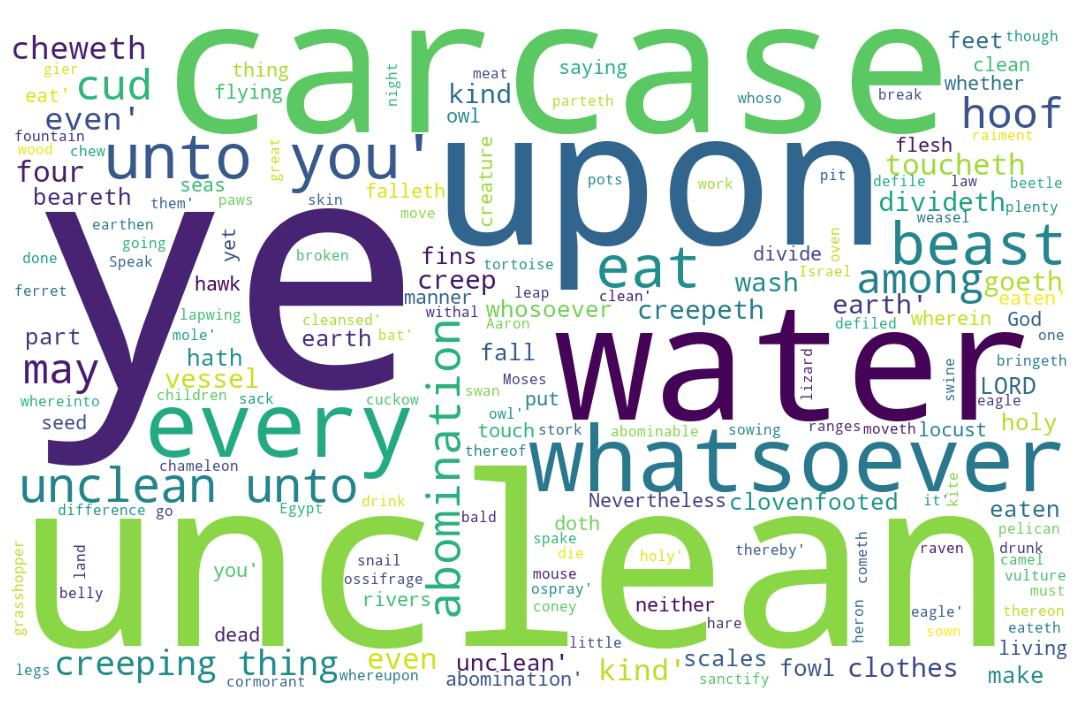
\includegraphics[width=\linewidth]{03OT-Leviticus/Leviticus11-WordCloud.jpg}
  \caption{Leviticus 11 Word Cloud}
  \label{fig:Leviticus 11 word Cloud}
\end{figure}

\marginpar{\scriptsize \centering \fcolorbox{black}{lime}{\textbf{DIFFERENCES \& DIVISION}}\\ (Leviticus 11:1--47) 
\begin{compactenum}[I.][8]
    \item \textbf{Unclean} \index[scripture]{Leviticus!Lev 11:04} (Lev 11:4) (word used 32 times in chapter)
    \item \textbf{Untouchable} \index[scripture]{Leviticus!Lev 11:08}\index[scripture]{Leviticus!Lev 11:24}\index[scripture]{Leviticus!Lev 11:26}\index[scripture]{Leviticus!Lev 11:27}\index[scripture]{Leviticus!Lev 11:31}\index[scripture]{Leviticus!Lev 11:36}\index[scripture]{Leviticus!Lev 11:39} (Lev 11:8, 24, 26, 27, 31, 36, 39)
    \item \textbf{Understanding} \index[scripture]{Leviticus!Lev 11:47} (Lev 11:47) (we must care about this!)
    \begin{compactenum}[A.][7]
    	\item The differences
    	\item The direction
    	\item The determination
    	\item The decisions
    	\item The discernment
    \end{compactenum}
    \item \textbf{Undefiled} (stay undefiled)
    \begin{compactenum}[A.][7]
    	\item In principle
    	\item In practice
    	\item In priority
    \end{compactenum}
    \item \textbf{Unprofitable} (do what makes a difference)
    \item \textbf{Unedifying} 
\end{compactenum} }

%%%%%%%%%%%%%%%%%%%%%%%%%%%%%%
%%%%%%%%%%%%%%%%%%%%%%%%%%%%%%
\footnote{\textcolor[cmyk]{0.99998,1,0,0}{\hyperlink{TOC}{Return to end of Table of Contents.}}}\footnote{\href{https://audiobible.com/bible/leviticus_11.html}{\textcolor[cmyk]{0.99998,1,0,0}{Leviticus 11 Audio}}}\textcolor[cmyk]{0.99998,1,0,0}{And the LORD spake unto Moses and to Aaron, saying unto them,}
[2] \textcolor[cmyk]{0.99998,1,0,0}{Speak unto the children of Israel, saying, These \emph{are} the beasts which ye shall eat among all the beasts that \emph{are} on the earth.}
[3] \textcolor[cmyk]{0.99998,1,0,0}{Whatsoever parteth the hoof, and is clovenfooted, \emph{and} cheweth the cud, among the beasts, that shall ye eat.}
[4] \textcolor[cmyk]{0.99998,1,0,0}{Nevertheless these shall ye not eat of them that chew the cud, or of them that divide the hoof: \emph{as} the camel, because he cheweth the cud, but divideth not the hoof; he \emph{is} \fcolorbox{black}{lime}{unclean} unto you.}
[5] \textcolor[cmyk]{0.99998,1,0,0}{And the coney, because he cheweth the cud, but divideth not the hoof; he \emph{is} unclean unto you.}
[6] \textcolor[cmyk]{0.99998,1,0,0}{And the hare, because he cheweth the cud, but divideth not the hoof; he \emph{is} unclean unto you.}
[7] \textcolor[cmyk]{0.99998,1,0,0}{And the swine, though he divide the hoof, and be clovenfooted, yet he cheweth not the cud; he \emph{is} unclean to you.}
[8] \textcolor[cmyk]{0.99998,1,0,0}{Of their flesh shall ye not eat, and their carcase shall ye \fcolorbox{black}{lime}{not touch}; they \emph{are} unclean to you.}\\
\\
\P \textcolor[cmyk]{0.99998,1,0,0}{These shall ye eat of all that \emph{are} in the waters: whatsoever hath fins and scales in the waters, in the seas, and in the rivers, them shall ye eat.}
[10] \textcolor[cmyk]{0.99998,1,0,0}{And all that have not fins and scales in the seas, and in the rivers, of all that move in the waters, and of any living thing which \emph{is} in the waters, they \emph{shall} \emph{be} an abomination unto you:}
[11] \textcolor[cmyk]{0.99998,1,0,0}{They shall be even an abomination unto you; ye shall not eat of their flesh, but ye shall have their carcases in abomination.}
[12] \textcolor[cmyk]{0.99998,1,0,0}{Whatsoever hath no fins nor scales in the waters, that \emph{shall} \emph{be} an abomination unto you.}\\
\\
\P \textcolor[cmyk]{0.99998,1,0,0}{And these \emph{are} \emph{they} \emph{which} ye shall have in abomination among the fowls; they shall not be eaten, they \emph{are} an abomination: the eagle, and the ossifrage, and the ospray,}
[14] \textcolor[cmyk]{0.99998,1,0,0}{And the vulture, and the kite after his kind;}
[15] \textcolor[cmyk]{0.99998,1,0,0}{Every raven after his kind;}
[16] \textcolor[cmyk]{0.99998,1,0,0}{And the owl, and the night hawk, and the cuckow, and the hawk after his kind,}
[17] \textcolor[cmyk]{0.99998,1,0,0}{And the little owl, and the cormorant, and the great owl,}
[18] \textcolor[cmyk]{0.99998,1,0,0}{And the swan, and the pelican, and the gier eagle,}
[19] \textcolor[cmyk]{0.99998,1,0,0}{And the stork, the heron after her kind, and the lapwing, and the bat.}
[20] \textcolor[cmyk]{0.99998,1,0,0}{All fowls that creep, going upon \emph{all} four, \emph{shall} \emph{be} an abomination unto you.}
[21] \textcolor[cmyk]{0.99998,1,0,0}{Yet these may ye eat of every flying creeping thing that goeth upon \emph{all} four, which have legs above their feet, to leap withal upon the earth;}
[22] \textcolor[cmyk]{0.99998,1,0,0}{\emph{Even} these of them ye may eat; the locust after his kind, and the bald locust after his kind, and the beetle after his kind, and the grasshopper after his kind.}
[23] \textcolor[cmyk]{0.99998,1,0,0}{But all \emph{other} flying creeping things, which have four feet, \emph{shall} \emph{be} an abomination unto you.}
[24] \textcolor[cmyk]{0.99998,1,0,0}{And for these ye shall be unclean: whosoever toucheth the carcase of them shall be unclean until the even.}
[25] \textcolor[cmyk]{0.99998,1,0,0}{And whosoever beareth \emph{ought} of the carcase of them shall wash his clothes, and be unclean until the even.}
[26] \textcolor[cmyk]{0.99998,1,0,0}{\emph{The} \emph{carcases} of every beast which divideth the hoof, and \emph{is} not clovenfooted, nor cheweth the cud, \emph{are} unclean unto you: every one that toucheth them shall be unclean.}
[27] \textcolor[cmyk]{0.99998,1,0,0}{And whatsoever goeth upon his paws, among all manner of beasts that go on \emph{all} four, those \emph{are} unclean unto you: whoso toucheth their carcase shall be unclean until the even.}
[28] \textcolor[cmyk]{0.99998,1,0,0}{And he that beareth the carcase of them shall wash his clothes, and be unclean until the even: they \emph{are} unclean unto you.}\\
\\
\P \textcolor[cmyk]{0.99998,1,0,0}{These also \emph{shall} \emph{be} unclean unto you among the creeping things that creep upon the earth; the weasel, and the mouse, and the tortoise after his kind,}
[30] \textcolor[cmyk]{0.99998,1,0,0}{And the ferret, and the chameleon, and the lizard, and the snail, and the mole.}
[31] \textcolor[cmyk]{0.99998,1,0,0}{These \emph{are} unclean to you among all that creep: whosoever doth touch them, when they be dead, shall be unclean until the even.}
[32] \textcolor[cmyk]{0.99998,1,0,0}{And upon whatsoever \emph{any} of them, when they are dead, doth fall, it shall be unclean; whether \emph{it} \emph{be} any vessel of wood, or raiment, or skin, or sack, whatsoever vessel \emph{it} \emph{be}, wherein \emph{any} work is done, it must be put into water, and it shall be unclean until the even; so it shall be cleansed.}
[33] \textcolor[cmyk]{0.99998,1,0,0}{And every earthen vessel, whereinto \emph{any} of them falleth, whatsoever \emph{is} in it shall be unclean; and ye shall break it.}
[34] \textcolor[cmyk]{0.99998,1,0,0}{Of all meat which may be eaten, \emph{that} on which \emph{such} water cometh shall be unclean: and all drink that may be drunk in every \emph{such} vessel shall be unclean.}
[35] \textcolor[cmyk]{0.99998,1,0,0}{And every \emph{thing} whereupon \emph{any} \emph{part} of their carcase falleth shall be unclean; \emph{whether} \emph{it} \emph{be} oven, or ranges for pots, they shall be broken down: \emph{for} they \emph{are} unclean, and shall be unclean unto you.}
[36] \textcolor[cmyk]{0.99998,1,0,0}{Nevertheless a fountain or pit, \emph{wherein} \emph{there} \emph{is} plenty of water, shall be clean: but that which toucheth their carcase shall be unclean.}
[37] \textcolor[cmyk]{0.99998,1,0,0}{And if \emph{any} \emph{part} of their carcase fall upon any sowing seed which is to be sown, it \emph{shall} \emph{be} clean.}
[38] \textcolor[cmyk]{0.99998,1,0,0}{But if \emph{any} water be put upon the seed, and \emph{any} \emph{part} of their carcase fall thereon, it \emph{shall} \emph{be} unclean unto you.}
[39] \textcolor[cmyk]{0.99998,1,0,0}{And if any beast, of which ye may eat, die; he that toucheth the carcase thereof shall be unclean until the even.}
[40] \textcolor[cmyk]{0.99998,1,0,0}{And he that eateth of the carcase of it shall wash his clothes, and be unclean until the even: he also that beareth the carcase of it shall wash his clothes, and be unclean until the even.}
[41] \textcolor[cmyk]{0.99998,1,0,0}{And every creeping thing that creepeth upon the earth \emph{shall} \emph{be} an abomination; it shall not be eaten.}
[42] \textcolor[cmyk]{0.99998,1,0,0}{Whatsoever goeth upon the belly, and whatsoever goeth upon \emph{all} four, or whatsoever hath more feet among all creeping things that creep upon the earth, them ye shall not eat; for they \emph{are} an abomination.}
[43] \textcolor[cmyk]{0.99998,1,0,0}{Ye shall not make yourselves abominable with any creeping thing that creepeth, neither shall ye make yourselves unclean with them, that ye should be defiled thereby.}
[44] \textcolor[cmyk]{0.99998,1,0,0}{For I \emph{am} the LORD your God: ye shall therefore sanctify yourselves, and ye shall be holy; for I \emph{am} holy: neither shall ye defile yourselves with any manner of creeping thing that creepeth upon the earth.}
[45] \textcolor[cmyk]{0.99998,1,0,0}{For I \emph{am} the LORD that bringeth you up out of the land of Egypt, to be your God: ye shall therefore be holy, for I \emph{am} holy.}
[46] \textcolor[cmyk]{0.99998,1,0,0}{This \emph{is} the law of the beasts, and of the fowl, and of every living creature that moveth in the waters, and of every creature that creepeth upon the earth:}
[47] \textcolor[cmyk]{0.99998,1,0,0}{To make a \fcolorbox{black}{lime}{difference} between the unclean and the clean, and between the beast that may be eaten and the beast that may not be eaten.}
\index[NWIV]{12!Leviticus!Lev 11:1}\index[AWIP]{And!Leviticus!Lev 11:1}\index[AWIP]{the!Leviticus!Lev 11:1}\index[AWIP]{LORD!Leviticus!Lev 11:1}\index[AWIP]{spake!Leviticus!Lev 11:1}\index[AWIP]{unto!Leviticus!Lev 11:1}\index[AWIP]{unto!Leviticus!Lev 11:1 (2)}\index[AWIP]{Moses!Leviticus!Lev 11:1}\index[AWIP]{and!Leviticus!Lev 11:1}\index[AWIP]{to!Leviticus!Lev 11:1}\index[AWIP]{Aaron!Leviticus!Lev 11:1}\index[AWIP]{saying!Leviticus!Lev 11:1}\index[AWIP]{them!Leviticus!Lev 11:1}

\index[NWIV]{24!Leviticus!Lev 11:2}\index[AWIP]{Speak!Leviticus!Lev 11:2}\index[AWIP]{unto!Leviticus!Lev 11:2}\index[AWIP]{the!Leviticus!Lev 11:2}\index[AWIP]{the!Leviticus!Lev 11:2 (2)}\index[AWIP]{the!Leviticus!Lev 11:2 (3)}\index[AWIP]{the!Leviticus!Lev 11:2 (4)}\index[AWIP]{children!Leviticus!Lev 11:2}\index[AWIP]{of!Leviticus!Lev 11:2}\index[AWIP]{Israel!Leviticus!Lev 11:2}\index[AWIP]{saying!Leviticus!Lev 11:2}\index[AWIP]{These!Leviticus!Lev 11:2}\index[AWIP]{\emph{are}!Leviticus!Lev 11:2}\index[AWIP]{\emph{are}!Leviticus!Lev 11:2 (2)}\index[AWIP]{beasts!Leviticus!Lev 11:2}\index[AWIP]{beasts!Leviticus!Lev 11:2 (2)}\index[AWIP]{which!Leviticus!Lev 11:2}\index[AWIP]{ye!Leviticus!Lev 11:2}\index[AWIP]{shall!Leviticus!Lev 11:2}\index[AWIP]{eat!Leviticus!Lev 11:2}\index[AWIP]{among!Leviticus!Lev 11:2}\index[AWIP]{all!Leviticus!Lev 11:2}\index[AWIP]{that!Leviticus!Lev 11:2}\index[AWIP]{on!Leviticus!Lev 11:2}\index[AWIP]{earth!Leviticus!Lev 11:2}\index[AWIP]{\emph{are}!Leviticus!Lev 11:2}\index[AWIP]{\emph{are}!Leviticus!Lev 11:2 (2)}

\index[NWIV]{18!Leviticus!Lev 11:3}\index[AWIP]{Whatsoever!Leviticus!Lev 11:3}\index[AWIP]{parteth!Leviticus!Lev 11:3}\index[AWIP]{the!Leviticus!Lev 11:3}\index[AWIP]{the!Leviticus!Lev 11:3 (2)}\index[AWIP]{the!Leviticus!Lev 11:3 (3)}\index[AWIP]{hoof!Leviticus!Lev 11:3}\index[AWIP]{and!Leviticus!Lev 11:3}\index[AWIP]{is!Leviticus!Lev 11:3}\index[AWIP]{clovenfooted!Leviticus!Lev 11:3}\index[AWIP]{\emph{and}!Leviticus!Lev 11:3}\index[AWIP]{cheweth!Leviticus!Lev 11:3}\index[AWIP]{cud!Leviticus!Lev 11:3}\index[AWIP]{among!Leviticus!Lev 11:3}\index[AWIP]{beasts!Leviticus!Lev 11:3}\index[AWIP]{that!Leviticus!Lev 11:3}\index[AWIP]{shall!Leviticus!Lev 11:3}\index[AWIP]{ye!Leviticus!Lev 11:3}\index[AWIP]{eat!Leviticus!Lev 11:3}\index[AWIP]{\emph{and}!Leviticus!Lev 11:3}

\index[NWIV]{37!Leviticus!Lev 11:4}\index[AWIP]{Nevertheless!Leviticus!Lev 11:4}\index[AWIP]{these!Leviticus!Lev 11:4}\index[AWIP]{shall!Leviticus!Lev 11:4}\index[AWIP]{ye!Leviticus!Lev 11:4}\index[AWIP]{not!Leviticus!Lev 11:4}\index[AWIP]{not!Leviticus!Lev 11:4 (2)}\index[AWIP]{eat!Leviticus!Lev 11:4}\index[AWIP]{of!Leviticus!Lev 11:4}\index[AWIP]{of!Leviticus!Lev 11:4 (2)}\index[AWIP]{them!Leviticus!Lev 11:4}\index[AWIP]{them!Leviticus!Lev 11:4 (2)}\index[AWIP]{that!Leviticus!Lev 11:4}\index[AWIP]{that!Leviticus!Lev 11:4 (2)}\index[AWIP]{chew!Leviticus!Lev 11:4}\index[AWIP]{the!Leviticus!Lev 11:4}\index[AWIP]{the!Leviticus!Lev 11:4 (2)}\index[AWIP]{the!Leviticus!Lev 11:4 (3)}\index[AWIP]{the!Leviticus!Lev 11:4 (4)}\index[AWIP]{the!Leviticus!Lev 11:4 (5)}\index[AWIP]{cud!Leviticus!Lev 11:4}\index[AWIP]{cud!Leviticus!Lev 11:4 (2)}\index[AWIP]{or!Leviticus!Lev 11:4}\index[AWIP]{divide!Leviticus!Lev 11:4}\index[AWIP]{hoof!Leviticus!Lev 11:4}\index[AWIP]{hoof!Leviticus!Lev 11:4 (2)}\index[AWIP]{\emph{as}!Leviticus!Lev 11:4}\index[AWIP]{camel!Leviticus!Lev 11:4}\index[AWIP]{because!Leviticus!Lev 11:4}\index[AWIP]{he!Leviticus!Lev 11:4}\index[AWIP]{he!Leviticus!Lev 11:4 (2)}\index[AWIP]{cheweth!Leviticus!Lev 11:4}\index[AWIP]{but!Leviticus!Lev 11:4}\index[AWIP]{divideth!Leviticus!Lev 11:4}\index[AWIP]{\emph{is}!Leviticus!Lev 11:4}\index[AWIP]{unclean!Leviticus!Lev 11:4}\index[AWIP]{unto!Leviticus!Lev 11:4}\index[AWIP]{you!Leviticus!Lev 11:4}\index[AWIP]{\emph{as}!Leviticus!Lev 11:4}\index[AWIP]{\emph{is}!Leviticus!Lev 11:4}

\index[NWIV]{18!Leviticus!Lev 11:5}\index[AWIP]{And!Leviticus!Lev 11:5}\index[AWIP]{the!Leviticus!Lev 11:5}\index[AWIP]{the!Leviticus!Lev 11:5 (2)}\index[AWIP]{the!Leviticus!Lev 11:5 (3)}\index[AWIP]{coney!Leviticus!Lev 11:5}\index[AWIP]{because!Leviticus!Lev 11:5}\index[AWIP]{he!Leviticus!Lev 11:5}\index[AWIP]{he!Leviticus!Lev 11:5 (2)}\index[AWIP]{cheweth!Leviticus!Lev 11:5}\index[AWIP]{cud!Leviticus!Lev 11:5}\index[AWIP]{but!Leviticus!Lev 11:5}\index[AWIP]{divideth!Leviticus!Lev 11:5}\index[AWIP]{not!Leviticus!Lev 11:5}\index[AWIP]{hoof!Leviticus!Lev 11:5}\index[AWIP]{\emph{is}!Leviticus!Lev 11:5}\index[AWIP]{unclean!Leviticus!Lev 11:5}\index[AWIP]{unto!Leviticus!Lev 11:5}\index[AWIP]{you!Leviticus!Lev 11:5}\index[AWIP]{\emph{is}!Leviticus!Lev 11:5}

\index[NWIV]{18!Leviticus!Lev 11:6}\index[AWIP]{And!Leviticus!Lev 11:6}\index[AWIP]{the!Leviticus!Lev 11:6}\index[AWIP]{the!Leviticus!Lev 11:6 (2)}\index[AWIP]{the!Leviticus!Lev 11:6 (3)}\index[AWIP]{hare!Leviticus!Lev 11:6}\index[AWIP]{because!Leviticus!Lev 11:6}\index[AWIP]{he!Leviticus!Lev 11:6}\index[AWIP]{he!Leviticus!Lev 11:6 (2)}\index[AWIP]{cheweth!Leviticus!Lev 11:6}\index[AWIP]{cud!Leviticus!Lev 11:6}\index[AWIP]{but!Leviticus!Lev 11:6}\index[AWIP]{divideth!Leviticus!Lev 11:6}\index[AWIP]{not!Leviticus!Lev 11:6}\index[AWIP]{hoof!Leviticus!Lev 11:6}\index[AWIP]{\emph{is}!Leviticus!Lev 11:6}\index[AWIP]{unclean!Leviticus!Lev 11:6}\index[AWIP]{unto!Leviticus!Lev 11:6}\index[AWIP]{you!Leviticus!Lev 11:6}\index[AWIP]{\emph{is}!Leviticus!Lev 11:6}

\index[NWIV]{22!Leviticus!Lev 11:7}\index[AWIP]{And!Leviticus!Lev 11:7}\index[AWIP]{the!Leviticus!Lev 11:7}\index[AWIP]{the!Leviticus!Lev 11:7 (2)}\index[AWIP]{the!Leviticus!Lev 11:7 (3)}\index[AWIP]{swine!Leviticus!Lev 11:7}\index[AWIP]{though!Leviticus!Lev 11:7}\index[AWIP]{he!Leviticus!Lev 11:7}\index[AWIP]{he!Leviticus!Lev 11:7 (2)}\index[AWIP]{he!Leviticus!Lev 11:7 (3)}\index[AWIP]{divide!Leviticus!Lev 11:7}\index[AWIP]{hoof!Leviticus!Lev 11:7}\index[AWIP]{and!Leviticus!Lev 11:7}\index[AWIP]{be!Leviticus!Lev 11:7}\index[AWIP]{clovenfooted!Leviticus!Lev 11:7}\index[AWIP]{yet!Leviticus!Lev 11:7}\index[AWIP]{cheweth!Leviticus!Lev 11:7}\index[AWIP]{not!Leviticus!Lev 11:7}\index[AWIP]{cud!Leviticus!Lev 11:7}\index[AWIP]{\emph{is}!Leviticus!Lev 11:7}\index[AWIP]{unclean!Leviticus!Lev 11:7}\index[AWIP]{to!Leviticus!Lev 11:7}\index[AWIP]{you!Leviticus!Lev 11:7}\index[AWIP]{\emph{is}!Leviticus!Lev 11:7}

\index[NWIV]{19!Leviticus!Lev 11:8}\index[AWIP]{Of!Leviticus!Lev 11:8}\index[AWIP]{their!Leviticus!Lev 11:8}\index[AWIP]{their!Leviticus!Lev 11:8 (2)}\index[AWIP]{flesh!Leviticus!Lev 11:8}\index[AWIP]{shall!Leviticus!Lev 11:8}\index[AWIP]{shall!Leviticus!Lev 11:8 (2)}\index[AWIP]{ye!Leviticus!Lev 11:8}\index[AWIP]{ye!Leviticus!Lev 11:8 (2)}\index[AWIP]{not!Leviticus!Lev 11:8}\index[AWIP]{not!Leviticus!Lev 11:8 (2)}\index[AWIP]{eat!Leviticus!Lev 11:8}\index[AWIP]{and!Leviticus!Lev 11:8}\index[AWIP]{carcase!Leviticus!Lev 11:8}\index[AWIP]{touch!Leviticus!Lev 11:8}\index[AWIP]{they!Leviticus!Lev 11:8}\index[AWIP]{\emph{are}!Leviticus!Lev 11:8}\index[AWIP]{unclean!Leviticus!Lev 11:8}\index[AWIP]{to!Leviticus!Lev 11:8}\index[AWIP]{you!Leviticus!Lev 11:8}\index[AWIP]{\emph{are}!Leviticus!Lev 11:8}

\index[NWIV]{30!Leviticus!Lev 11:9}\index[AWIP]{These!Leviticus!Lev 11:9}\index[AWIP]{shall!Leviticus!Lev 11:9}\index[AWIP]{shall!Leviticus!Lev 11:9 (2)}\index[AWIP]{ye!Leviticus!Lev 11:9}\index[AWIP]{ye!Leviticus!Lev 11:9 (2)}\index[AWIP]{eat!Leviticus!Lev 11:9}\index[AWIP]{eat!Leviticus!Lev 11:9 (2)}\index[AWIP]{of!Leviticus!Lev 11:9}\index[AWIP]{all!Leviticus!Lev 11:9}\index[AWIP]{that!Leviticus!Lev 11:9}\index[AWIP]{\emph{are}!Leviticus!Lev 11:9}\index[AWIP]{in!Leviticus!Lev 11:9}\index[AWIP]{in!Leviticus!Lev 11:9 (2)}\index[AWIP]{in!Leviticus!Lev 11:9 (3)}\index[AWIP]{in!Leviticus!Lev 11:9 (4)}\index[AWIP]{the!Leviticus!Lev 11:9}\index[AWIP]{the!Leviticus!Lev 11:9 (2)}\index[AWIP]{the!Leviticus!Lev 11:9 (3)}\index[AWIP]{the!Leviticus!Lev 11:9 (4)}\index[AWIP]{waters!Leviticus!Lev 11:9}\index[AWIP]{waters!Leviticus!Lev 11:9 (2)}\index[AWIP]{whatsoever!Leviticus!Lev 11:9}\index[AWIP]{hath!Leviticus!Lev 11:9}\index[AWIP]{fins!Leviticus!Lev 11:9}\index[AWIP]{and!Leviticus!Lev 11:9}\index[AWIP]{and!Leviticus!Lev 11:9 (2)}\index[AWIP]{scales!Leviticus!Lev 11:9}\index[AWIP]{seas!Leviticus!Lev 11:9}\index[AWIP]{rivers!Leviticus!Lev 11:9}\index[AWIP]{them!Leviticus!Lev 11:9}\index[AWIP]{\emph{are}!Leviticus!Lev 11:9}

\index[NWIV]{39!Leviticus!Lev 11:10}\index[AWIP]{And!Leviticus!Lev 11:10}\index[AWIP]{all!Leviticus!Lev 11:10}\index[AWIP]{all!Leviticus!Lev 11:10 (2)}\index[AWIP]{that!Leviticus!Lev 11:10}\index[AWIP]{that!Leviticus!Lev 11:10 (2)}\index[AWIP]{have!Leviticus!Lev 11:10}\index[AWIP]{not!Leviticus!Lev 11:10}\index[AWIP]{fins!Leviticus!Lev 11:10}\index[AWIP]{and!Leviticus!Lev 11:10}\index[AWIP]{and!Leviticus!Lev 11:10 (2)}\index[AWIP]{and!Leviticus!Lev 11:10 (3)}\index[AWIP]{scales!Leviticus!Lev 11:10}\index[AWIP]{in!Leviticus!Lev 11:10}\index[AWIP]{in!Leviticus!Lev 11:10 (2)}\index[AWIP]{in!Leviticus!Lev 11:10 (3)}\index[AWIP]{in!Leviticus!Lev 11:10 (4)}\index[AWIP]{the!Leviticus!Lev 11:10}\index[AWIP]{the!Leviticus!Lev 11:10 (2)}\index[AWIP]{the!Leviticus!Lev 11:10 (3)}\index[AWIP]{the!Leviticus!Lev 11:10 (4)}\index[AWIP]{seas!Leviticus!Lev 11:10}\index[AWIP]{rivers!Leviticus!Lev 11:10}\index[AWIP]{of!Leviticus!Lev 11:10}\index[AWIP]{of!Leviticus!Lev 11:10 (2)}\index[AWIP]{move!Leviticus!Lev 11:10}\index[AWIP]{waters!Leviticus!Lev 11:10}\index[AWIP]{waters!Leviticus!Lev 11:10 (2)}\index[AWIP]{any!Leviticus!Lev 11:10}\index[AWIP]{living!Leviticus!Lev 11:10}\index[AWIP]{thing!Leviticus!Lev 11:10}\index[AWIP]{which!Leviticus!Lev 11:10}\index[AWIP]{\emph{is}!Leviticus!Lev 11:10}\index[AWIP]{they!Leviticus!Lev 11:10}\index[AWIP]{\emph{shall}!Leviticus!Lev 11:10}\index[AWIP]{\emph{be}!Leviticus!Lev 11:10}\index[AWIP]{an!Leviticus!Lev 11:10}\index[AWIP]{abomination!Leviticus!Lev 11:10}\index[AWIP]{unto!Leviticus!Lev 11:10}\index[AWIP]{you!Leviticus!Lev 11:10}\index[AWIP]{\emph{is}!Leviticus!Lev 11:10}\index[AWIP]{\emph{shall}!Leviticus!Lev 11:10}\index[AWIP]{\emph{be}!Leviticus!Lev 11:10}

\index[NWIV]{23!Leviticus!Lev 11:11}\index[AWIP]{They!Leviticus!Lev 11:11}\index[AWIP]{shall!Leviticus!Lev 11:11}\index[AWIP]{shall!Leviticus!Lev 11:11 (2)}\index[AWIP]{shall!Leviticus!Lev 11:11 (3)}\index[AWIP]{be!Leviticus!Lev 11:11}\index[AWIP]{even!Leviticus!Lev 11:11}\index[AWIP]{an!Leviticus!Lev 11:11}\index[AWIP]{abomination!Leviticus!Lev 11:11}\index[AWIP]{abomination!Leviticus!Lev 11:11 (2)}\index[AWIP]{unto!Leviticus!Lev 11:11}\index[AWIP]{you!Leviticus!Lev 11:11}\index[AWIP]{ye!Leviticus!Lev 11:11}\index[AWIP]{ye!Leviticus!Lev 11:11 (2)}\index[AWIP]{not!Leviticus!Lev 11:11}\index[AWIP]{eat!Leviticus!Lev 11:11}\index[AWIP]{of!Leviticus!Lev 11:11}\index[AWIP]{their!Leviticus!Lev 11:11}\index[AWIP]{their!Leviticus!Lev 11:11 (2)}\index[AWIP]{flesh!Leviticus!Lev 11:11}\index[AWIP]{but!Leviticus!Lev 11:11}\index[AWIP]{have!Leviticus!Lev 11:11}\index[AWIP]{carcases!Leviticus!Lev 11:11}\index[AWIP]{in!Leviticus!Lev 11:11}

\index[NWIV]{16!Leviticus!Lev 11:12}\index[AWIP]{Whatsoever!Leviticus!Lev 11:12}\index[AWIP]{hath!Leviticus!Lev 11:12}\index[AWIP]{no!Leviticus!Lev 11:12}\index[AWIP]{fins!Leviticus!Lev 11:12}\index[AWIP]{nor!Leviticus!Lev 11:12}\index[AWIP]{scales!Leviticus!Lev 11:12}\index[AWIP]{in!Leviticus!Lev 11:12}\index[AWIP]{the!Leviticus!Lev 11:12}\index[AWIP]{waters!Leviticus!Lev 11:12}\index[AWIP]{that!Leviticus!Lev 11:12}\index[AWIP]{\emph{shall}!Leviticus!Lev 11:12}\index[AWIP]{\emph{be}!Leviticus!Lev 11:12}\index[AWIP]{an!Leviticus!Lev 11:12}\index[AWIP]{abomination!Leviticus!Lev 11:12}\index[AWIP]{unto!Leviticus!Lev 11:12}\index[AWIP]{you!Leviticus!Lev 11:12}\index[AWIP]{\emph{shall}!Leviticus!Lev 11:12}\index[AWIP]{\emph{be}!Leviticus!Lev 11:12}

\index[NWIV]{30!Leviticus!Lev 11:13}\index[AWIP]{And!Leviticus!Lev 11:13}\index[AWIP]{these!Leviticus!Lev 11:13}\index[AWIP]{\emph{are}!Leviticus!Lev 11:13}\index[AWIP]{\emph{are}!Leviticus!Lev 11:13 (2)}\index[AWIP]{\emph{they}!Leviticus!Lev 11:13}\index[AWIP]{\emph{which}!Leviticus!Lev 11:13}\index[AWIP]{ye!Leviticus!Lev 11:13}\index[AWIP]{shall!Leviticus!Lev 11:13}\index[AWIP]{shall!Leviticus!Lev 11:13 (2)}\index[AWIP]{have!Leviticus!Lev 11:13}\index[AWIP]{in!Leviticus!Lev 11:13}\index[AWIP]{abomination!Leviticus!Lev 11:13}\index[AWIP]{abomination!Leviticus!Lev 11:13 (2)}\index[AWIP]{among!Leviticus!Lev 11:13}\index[AWIP]{the!Leviticus!Lev 11:13}\index[AWIP]{the!Leviticus!Lev 11:13 (2)}\index[AWIP]{the!Leviticus!Lev 11:13 (3)}\index[AWIP]{the!Leviticus!Lev 11:13 (4)}\index[AWIP]{fowls!Leviticus!Lev 11:13}\index[AWIP]{they!Leviticus!Lev 11:13}\index[AWIP]{they!Leviticus!Lev 11:13 (2)}\index[AWIP]{not!Leviticus!Lev 11:13}\index[AWIP]{be!Leviticus!Lev 11:13}\index[AWIP]{eaten!Leviticus!Lev 11:13}\index[AWIP]{an!Leviticus!Lev 11:13}\index[AWIP]{eagle!Leviticus!Lev 11:13}\index[AWIP]{and!Leviticus!Lev 11:13}\index[AWIP]{and!Leviticus!Lev 11:13 (2)}\index[AWIP]{ossifrage!Leviticus!Lev 11:13}\index[AWIP]{ospray!Leviticus!Lev 11:13}\index[AWIP]{\emph{are}!Leviticus!Lev 11:13}\index[AWIP]{\emph{are}!Leviticus!Lev 11:13 (2)}\index[AWIP]{\emph{they}!Leviticus!Lev 11:13}\index[AWIP]{\emph{which}!Leviticus!Lev 11:13}

\index[NWIV]{9!Leviticus!Lev 11:14}\index[AWIP]{And!Leviticus!Lev 11:14}\index[AWIP]{the!Leviticus!Lev 11:14}\index[AWIP]{the!Leviticus!Lev 11:14 (2)}\index[AWIP]{vulture!Leviticus!Lev 11:14}\index[AWIP]{and!Leviticus!Lev 11:14}\index[AWIP]{kite!Leviticus!Lev 11:14}\index[AWIP]{after!Leviticus!Lev 11:14}\index[AWIP]{his!Leviticus!Lev 11:14}\index[AWIP]{kind!Leviticus!Lev 11:14}

\index[NWIV]{5!Leviticus!Lev 11:15}\index[AWIP]{Every!Leviticus!Lev 11:15}\index[AWIP]{raven!Leviticus!Lev 11:15}\index[AWIP]{after!Leviticus!Lev 11:15}\index[AWIP]{his!Leviticus!Lev 11:15}\index[AWIP]{kind!Leviticus!Lev 11:15}

\index[NWIV]{16!Leviticus!Lev 11:16}\index[AWIP]{And!Leviticus!Lev 11:16}\index[AWIP]{the!Leviticus!Lev 11:16}\index[AWIP]{the!Leviticus!Lev 11:16 (2)}\index[AWIP]{the!Leviticus!Lev 11:16 (3)}\index[AWIP]{the!Leviticus!Lev 11:16 (4)}\index[AWIP]{owl!Leviticus!Lev 11:16}\index[AWIP]{and!Leviticus!Lev 11:16}\index[AWIP]{and!Leviticus!Lev 11:16 (2)}\index[AWIP]{and!Leviticus!Lev 11:16 (3)}\index[AWIP]{night!Leviticus!Lev 11:16}\index[AWIP]{hawk!Leviticus!Lev 11:16}\index[AWIP]{hawk!Leviticus!Lev 11:16 (2)}\index[AWIP]{cuckow!Leviticus!Lev 11:16}\index[AWIP]{after!Leviticus!Lev 11:16}\index[AWIP]{his!Leviticus!Lev 11:16}\index[AWIP]{kind!Leviticus!Lev 11:16}

\index[NWIV]{11!Leviticus!Lev 11:17}\index[AWIP]{And!Leviticus!Lev 11:17}\index[AWIP]{the!Leviticus!Lev 11:17}\index[AWIP]{the!Leviticus!Lev 11:17 (2)}\index[AWIP]{the!Leviticus!Lev 11:17 (3)}\index[AWIP]{little!Leviticus!Lev 11:17}\index[AWIP]{owl!Leviticus!Lev 11:17}\index[AWIP]{owl!Leviticus!Lev 11:17 (2)}\index[AWIP]{and!Leviticus!Lev 11:17}\index[AWIP]{and!Leviticus!Lev 11:17 (2)}\index[AWIP]{cormorant!Leviticus!Lev 11:17}\index[AWIP]{great!Leviticus!Lev 11:17}

\index[NWIV]{10!Leviticus!Lev 11:18}\index[AWIP]{And!Leviticus!Lev 11:18}\index[AWIP]{the!Leviticus!Lev 11:18}\index[AWIP]{the!Leviticus!Lev 11:18 (2)}\index[AWIP]{the!Leviticus!Lev 11:18 (3)}\index[AWIP]{swan!Leviticus!Lev 11:18}\index[AWIP]{and!Leviticus!Lev 11:18}\index[AWIP]{and!Leviticus!Lev 11:18 (2)}\index[AWIP]{pelican!Leviticus!Lev 11:18}\index[AWIP]{gier!Leviticus!Lev 11:18}\index[AWIP]{eagle!Leviticus!Lev 11:18}

\index[NWIV]{14!Leviticus!Lev 11:19}\index[AWIP]{And!Leviticus!Lev 11:19}\index[AWIP]{the!Leviticus!Lev 11:19}\index[AWIP]{the!Leviticus!Lev 11:19 (2)}\index[AWIP]{the!Leviticus!Lev 11:19 (3)}\index[AWIP]{the!Leviticus!Lev 11:19 (4)}\index[AWIP]{stork!Leviticus!Lev 11:19}\index[AWIP]{heron!Leviticus!Lev 11:19}\index[AWIP]{after!Leviticus!Lev 11:19}\index[AWIP]{her!Leviticus!Lev 11:19}\index[AWIP]{kind!Leviticus!Lev 11:19}\index[AWIP]{and!Leviticus!Lev 11:19}\index[AWIP]{and!Leviticus!Lev 11:19 (2)}\index[AWIP]{lapwing!Leviticus!Lev 11:19}\index[AWIP]{bat!Leviticus!Lev 11:19}

\index[NWIV]{14!Leviticus!Lev 11:20}\index[AWIP]{All!Leviticus!Lev 11:20}\index[AWIP]{fowls!Leviticus!Lev 11:20}\index[AWIP]{that!Leviticus!Lev 11:20}\index[AWIP]{creep!Leviticus!Lev 11:20}\index[AWIP]{going!Leviticus!Lev 11:20}\index[AWIP]{upon!Leviticus!Lev 11:20}\index[AWIP]{\emph{all}!Leviticus!Lev 11:20}\index[AWIP]{four!Leviticus!Lev 11:20}\index[AWIP]{\emph{shall}!Leviticus!Lev 11:20}\index[AWIP]{\emph{be}!Leviticus!Lev 11:20}\index[AWIP]{an!Leviticus!Lev 11:20}\index[AWIP]{abomination!Leviticus!Lev 11:20}\index[AWIP]{unto!Leviticus!Lev 11:20}\index[AWIP]{you!Leviticus!Lev 11:20}\index[AWIP]{\emph{all}!Leviticus!Lev 11:20}\index[AWIP]{\emph{shall}!Leviticus!Lev 11:20}\index[AWIP]{\emph{be}!Leviticus!Lev 11:20}

\index[NWIV]{27!Leviticus!Lev 11:21}\index[AWIP]{Yet!Leviticus!Lev 11:21}\index[AWIP]{these!Leviticus!Lev 11:21}\index[AWIP]{may!Leviticus!Lev 11:21}\index[AWIP]{ye!Leviticus!Lev 11:21}\index[AWIP]{eat!Leviticus!Lev 11:21}\index[AWIP]{of!Leviticus!Lev 11:21}\index[AWIP]{every!Leviticus!Lev 11:21}\index[AWIP]{flying!Leviticus!Lev 11:21}\index[AWIP]{creeping!Leviticus!Lev 11:21}\index[AWIP]{thing!Leviticus!Lev 11:21}\index[AWIP]{that!Leviticus!Lev 11:21}\index[AWIP]{goeth!Leviticus!Lev 11:21}\index[AWIP]{upon!Leviticus!Lev 11:21}\index[AWIP]{upon!Leviticus!Lev 11:21 (2)}\index[AWIP]{\emph{all}!Leviticus!Lev 11:21}\index[AWIP]{four!Leviticus!Lev 11:21}\index[AWIP]{which!Leviticus!Lev 11:21}\index[AWIP]{have!Leviticus!Lev 11:21}\index[AWIP]{legs!Leviticus!Lev 11:21}\index[AWIP]{above!Leviticus!Lev 11:21}\index[AWIP]{their!Leviticus!Lev 11:21}\index[AWIP]{feet!Leviticus!Lev 11:21}\index[AWIP]{to!Leviticus!Lev 11:21}\index[AWIP]{leap!Leviticus!Lev 11:21}\index[AWIP]{withal!Leviticus!Lev 11:21}\index[AWIP]{the!Leviticus!Lev 11:21}\index[AWIP]{earth!Leviticus!Lev 11:21}\index[AWIP]{\emph{all}!Leviticus!Lev 11:21}

\index[NWIV]{31!Leviticus!Lev 11:22}\index[AWIP]{\emph{Even}!Leviticus!Lev 11:22}\index[AWIP]{these!Leviticus!Lev 11:22}\index[AWIP]{of!Leviticus!Lev 11:22}\index[AWIP]{them!Leviticus!Lev 11:22}\index[AWIP]{ye!Leviticus!Lev 11:22}\index[AWIP]{may!Leviticus!Lev 11:22}\index[AWIP]{eat!Leviticus!Lev 11:22}\index[AWIP]{the!Leviticus!Lev 11:22}\index[AWIP]{the!Leviticus!Lev 11:22 (2)}\index[AWIP]{the!Leviticus!Lev 11:22 (3)}\index[AWIP]{the!Leviticus!Lev 11:22 (4)}\index[AWIP]{locust!Leviticus!Lev 11:22}\index[AWIP]{locust!Leviticus!Lev 11:22 (2)}\index[AWIP]{after!Leviticus!Lev 11:22}\index[AWIP]{after!Leviticus!Lev 11:22 (2)}\index[AWIP]{after!Leviticus!Lev 11:22 (3)}\index[AWIP]{after!Leviticus!Lev 11:22 (4)}\index[AWIP]{his!Leviticus!Lev 11:22}\index[AWIP]{his!Leviticus!Lev 11:22 (2)}\index[AWIP]{his!Leviticus!Lev 11:22 (3)}\index[AWIP]{his!Leviticus!Lev 11:22 (4)}\index[AWIP]{kind!Leviticus!Lev 11:22}\index[AWIP]{kind!Leviticus!Lev 11:22 (2)}\index[AWIP]{kind!Leviticus!Lev 11:22 (3)}\index[AWIP]{kind!Leviticus!Lev 11:22 (4)}\index[AWIP]{and!Leviticus!Lev 11:22}\index[AWIP]{and!Leviticus!Lev 11:22 (2)}\index[AWIP]{and!Leviticus!Lev 11:22 (3)}\index[AWIP]{bald!Leviticus!Lev 11:22}\index[AWIP]{beetle!Leviticus!Lev 11:22}\index[AWIP]{grasshopper!Leviticus!Lev 11:22}\index[AWIP]{\emph{Even}!Leviticus!Lev 11:22}

\index[NWIV]{16!Leviticus!Lev 11:23}\index[AWIP]{But!Leviticus!Lev 11:23}\index[AWIP]{all!Leviticus!Lev 11:23}\index[AWIP]{\emph{other}!Leviticus!Lev 11:23}\index[AWIP]{flying!Leviticus!Lev 11:23}\index[AWIP]{creeping!Leviticus!Lev 11:23}\index[AWIP]{things!Leviticus!Lev 11:23}\index[AWIP]{which!Leviticus!Lev 11:23}\index[AWIP]{have!Leviticus!Lev 11:23}\index[AWIP]{four!Leviticus!Lev 11:23}\index[AWIP]{feet!Leviticus!Lev 11:23}\index[AWIP]{\emph{shall}!Leviticus!Lev 11:23}\index[AWIP]{\emph{be}!Leviticus!Lev 11:23}\index[AWIP]{an!Leviticus!Lev 11:23}\index[AWIP]{abomination!Leviticus!Lev 11:23}\index[AWIP]{unto!Leviticus!Lev 11:23}\index[AWIP]{you!Leviticus!Lev 11:23}\index[AWIP]{\emph{other}!Leviticus!Lev 11:23}\index[AWIP]{\emph{shall}!Leviticus!Lev 11:23}\index[AWIP]{\emph{be}!Leviticus!Lev 11:23}

\index[NWIV]{19!Leviticus!Lev 11:24}\index[AWIP]{And!Leviticus!Lev 11:24}\index[AWIP]{for!Leviticus!Lev 11:24}\index[AWIP]{these!Leviticus!Lev 11:24}\index[AWIP]{ye!Leviticus!Lev 11:24}\index[AWIP]{shall!Leviticus!Lev 11:24}\index[AWIP]{shall!Leviticus!Lev 11:24 (2)}\index[AWIP]{be!Leviticus!Lev 11:24}\index[AWIP]{be!Leviticus!Lev 11:24 (2)}\index[AWIP]{unclean!Leviticus!Lev 11:24}\index[AWIP]{unclean!Leviticus!Lev 11:24 (2)}\index[AWIP]{whosoever!Leviticus!Lev 11:24}\index[AWIP]{toucheth!Leviticus!Lev 11:24}\index[AWIP]{the!Leviticus!Lev 11:24}\index[AWIP]{the!Leviticus!Lev 11:24 (2)}\index[AWIP]{carcase!Leviticus!Lev 11:24}\index[AWIP]{of!Leviticus!Lev 11:24}\index[AWIP]{them!Leviticus!Lev 11:24}\index[AWIP]{until!Leviticus!Lev 11:24}\index[AWIP]{even!Leviticus!Lev 11:24}

\index[NWIV]{19!Leviticus!Lev 11:25}\index[AWIP]{And!Leviticus!Lev 11:25}\index[AWIP]{whosoever!Leviticus!Lev 11:25}\index[AWIP]{beareth!Leviticus!Lev 11:25}\index[AWIP]{\emph{ought}!Leviticus!Lev 11:25}\index[AWIP]{of!Leviticus!Lev 11:25}\index[AWIP]{of!Leviticus!Lev 11:25 (2)}\index[AWIP]{the!Leviticus!Lev 11:25}\index[AWIP]{the!Leviticus!Lev 11:25 (2)}\index[AWIP]{carcase!Leviticus!Lev 11:25}\index[AWIP]{them!Leviticus!Lev 11:25}\index[AWIP]{shall!Leviticus!Lev 11:25}\index[AWIP]{wash!Leviticus!Lev 11:25}\index[AWIP]{his!Leviticus!Lev 11:25}\index[AWIP]{clothes!Leviticus!Lev 11:25}\index[AWIP]{and!Leviticus!Lev 11:25}\index[AWIP]{be!Leviticus!Lev 11:25}\index[AWIP]{unclean!Leviticus!Lev 11:25}\index[AWIP]{until!Leviticus!Lev 11:25}\index[AWIP]{even!Leviticus!Lev 11:25}\index[AWIP]{\emph{ought}!Leviticus!Lev 11:25}

\index[NWIV]{29!Leviticus!Lev 11:26}\index[AWIP]{\emph{The}!Leviticus!Lev 11:26}\index[AWIP]{\emph{carcases}!Leviticus!Lev 11:26}\index[AWIP]{of!Leviticus!Lev 11:26}\index[AWIP]{every!Leviticus!Lev 11:26}\index[AWIP]{every!Leviticus!Lev 11:26 (2)}\index[AWIP]{beast!Leviticus!Lev 11:26}\index[AWIP]{which!Leviticus!Lev 11:26}\index[AWIP]{divideth!Leviticus!Lev 11:26}\index[AWIP]{the!Leviticus!Lev 11:26}\index[AWIP]{the!Leviticus!Lev 11:26 (2)}\index[AWIP]{hoof!Leviticus!Lev 11:26}\index[AWIP]{and!Leviticus!Lev 11:26}\index[AWIP]{\emph{is}!Leviticus!Lev 11:26}\index[AWIP]{not!Leviticus!Lev 11:26}\index[AWIP]{clovenfooted!Leviticus!Lev 11:26}\index[AWIP]{nor!Leviticus!Lev 11:26}\index[AWIP]{cheweth!Leviticus!Lev 11:26}\index[AWIP]{cud!Leviticus!Lev 11:26}\index[AWIP]{\emph{are}!Leviticus!Lev 11:26}\index[AWIP]{unclean!Leviticus!Lev 11:26}\index[AWIP]{unclean!Leviticus!Lev 11:26 (2)}\index[AWIP]{unto!Leviticus!Lev 11:26}\index[AWIP]{you!Leviticus!Lev 11:26}\index[AWIP]{one!Leviticus!Lev 11:26}\index[AWIP]{that!Leviticus!Lev 11:26}\index[AWIP]{toucheth!Leviticus!Lev 11:26}\index[AWIP]{them!Leviticus!Lev 11:26}\index[AWIP]{shall!Leviticus!Lev 11:26}\index[AWIP]{be!Leviticus!Lev 11:26}\index[AWIP]{\emph{The}!Leviticus!Lev 11:26}\index[AWIP]{\emph{carcases}!Leviticus!Lev 11:26}\index[AWIP]{\emph{is}!Leviticus!Lev 11:26}\index[AWIP]{\emph{are}!Leviticus!Lev 11:26}

\index[NWIV]{31!Leviticus!Lev 11:27}\index[AWIP]{And!Leviticus!Lev 11:27}\index[AWIP]{whatsoever!Leviticus!Lev 11:27}\index[AWIP]{goeth!Leviticus!Lev 11:27}\index[AWIP]{upon!Leviticus!Lev 11:27}\index[AWIP]{his!Leviticus!Lev 11:27}\index[AWIP]{paws!Leviticus!Lev 11:27}\index[AWIP]{among!Leviticus!Lev 11:27}\index[AWIP]{all!Leviticus!Lev 11:27}\index[AWIP]{manner!Leviticus!Lev 11:27}\index[AWIP]{of!Leviticus!Lev 11:27}\index[AWIP]{beasts!Leviticus!Lev 11:27}\index[AWIP]{that!Leviticus!Lev 11:27}\index[AWIP]{go!Leviticus!Lev 11:27}\index[AWIP]{on!Leviticus!Lev 11:27}\index[AWIP]{\emph{all}!Leviticus!Lev 11:27}\index[AWIP]{four!Leviticus!Lev 11:27}\index[AWIP]{those!Leviticus!Lev 11:27}\index[AWIP]{\emph{are}!Leviticus!Lev 11:27}\index[AWIP]{unclean!Leviticus!Lev 11:27}\index[AWIP]{unclean!Leviticus!Lev 11:27 (2)}\index[AWIP]{unto!Leviticus!Lev 11:27}\index[AWIP]{you!Leviticus!Lev 11:27}\index[AWIP]{whoso!Leviticus!Lev 11:27}\index[AWIP]{toucheth!Leviticus!Lev 11:27}\index[AWIP]{their!Leviticus!Lev 11:27}\index[AWIP]{carcase!Leviticus!Lev 11:27}\index[AWIP]{shall!Leviticus!Lev 11:27}\index[AWIP]{be!Leviticus!Lev 11:27}\index[AWIP]{until!Leviticus!Lev 11:27}\index[AWIP]{the!Leviticus!Lev 11:27}\index[AWIP]{even!Leviticus!Lev 11:27}\index[AWIP]{\emph{all}!Leviticus!Lev 11:27}\index[AWIP]{\emph{are}!Leviticus!Lev 11:27}

\index[NWIV]{23!Leviticus!Lev 11:28}\index[AWIP]{And!Leviticus!Lev 11:28}\index[AWIP]{he!Leviticus!Lev 11:28}\index[AWIP]{that!Leviticus!Lev 11:28}\index[AWIP]{beareth!Leviticus!Lev 11:28}\index[AWIP]{the!Leviticus!Lev 11:28}\index[AWIP]{the!Leviticus!Lev 11:28 (2)}\index[AWIP]{carcase!Leviticus!Lev 11:28}\index[AWIP]{of!Leviticus!Lev 11:28}\index[AWIP]{them!Leviticus!Lev 11:28}\index[AWIP]{shall!Leviticus!Lev 11:28}\index[AWIP]{wash!Leviticus!Lev 11:28}\index[AWIP]{his!Leviticus!Lev 11:28}\index[AWIP]{clothes!Leviticus!Lev 11:28}\index[AWIP]{and!Leviticus!Lev 11:28}\index[AWIP]{be!Leviticus!Lev 11:28}\index[AWIP]{unclean!Leviticus!Lev 11:28}\index[AWIP]{unclean!Leviticus!Lev 11:28 (2)}\index[AWIP]{until!Leviticus!Lev 11:28}\index[AWIP]{even!Leviticus!Lev 11:28}\index[AWIP]{they!Leviticus!Lev 11:28}\index[AWIP]{\emph{are}!Leviticus!Lev 11:28}\index[AWIP]{unto!Leviticus!Lev 11:28}\index[AWIP]{you!Leviticus!Lev 11:28}\index[AWIP]{\emph{are}!Leviticus!Lev 11:28}

\index[NWIV]{27!Leviticus!Lev 11:29}\index[AWIP]{These!Leviticus!Lev 11:29}\index[AWIP]{also!Leviticus!Lev 11:29}\index[AWIP]{\emph{shall}!Leviticus!Lev 11:29}\index[AWIP]{\emph{be}!Leviticus!Lev 11:29}\index[AWIP]{unclean!Leviticus!Lev 11:29}\index[AWIP]{unto!Leviticus!Lev 11:29}\index[AWIP]{you!Leviticus!Lev 11:29}\index[AWIP]{among!Leviticus!Lev 11:29}\index[AWIP]{the!Leviticus!Lev 11:29}\index[AWIP]{the!Leviticus!Lev 11:29 (2)}\index[AWIP]{the!Leviticus!Lev 11:29 (3)}\index[AWIP]{the!Leviticus!Lev 11:29 (4)}\index[AWIP]{the!Leviticus!Lev 11:29 (5)}\index[AWIP]{creeping!Leviticus!Lev 11:29}\index[AWIP]{things!Leviticus!Lev 11:29}\index[AWIP]{that!Leviticus!Lev 11:29}\index[AWIP]{creep!Leviticus!Lev 11:29}\index[AWIP]{upon!Leviticus!Lev 11:29}\index[AWIP]{earth!Leviticus!Lev 11:29}\index[AWIP]{weasel!Leviticus!Lev 11:29}\index[AWIP]{and!Leviticus!Lev 11:29}\index[AWIP]{and!Leviticus!Lev 11:29 (2)}\index[AWIP]{mouse!Leviticus!Lev 11:29}\index[AWIP]{tortoise!Leviticus!Lev 11:29}\index[AWIP]{after!Leviticus!Lev 11:29}\index[AWIP]{his!Leviticus!Lev 11:29}\index[AWIP]{kind!Leviticus!Lev 11:29}\index[AWIP]{\emph{shall}!Leviticus!Lev 11:29}\index[AWIP]{\emph{be}!Leviticus!Lev 11:29}

\index[NWIV]{15!Leviticus!Lev 11:30}\index[AWIP]{And!Leviticus!Lev 11:30}\index[AWIP]{the!Leviticus!Lev 11:30}\index[AWIP]{the!Leviticus!Lev 11:30 (2)}\index[AWIP]{the!Leviticus!Lev 11:30 (3)}\index[AWIP]{the!Leviticus!Lev 11:30 (4)}\index[AWIP]{the!Leviticus!Lev 11:30 (5)}\index[AWIP]{ferret!Leviticus!Lev 11:30}\index[AWIP]{and!Leviticus!Lev 11:30}\index[AWIP]{and!Leviticus!Lev 11:30 (2)}\index[AWIP]{and!Leviticus!Lev 11:30 (3)}\index[AWIP]{and!Leviticus!Lev 11:30 (4)}\index[AWIP]{chameleon!Leviticus!Lev 11:30}\index[AWIP]{lizard!Leviticus!Lev 11:30}\index[AWIP]{snail!Leviticus!Lev 11:30}\index[AWIP]{mole!Leviticus!Lev 11:30}

\index[NWIV]{23!Leviticus!Lev 11:31}\index[AWIP]{These!Leviticus!Lev 11:31}\index[AWIP]{\emph{are}!Leviticus!Lev 11:31}\index[AWIP]{unclean!Leviticus!Lev 11:31}\index[AWIP]{unclean!Leviticus!Lev 11:31 (2)}\index[AWIP]{to!Leviticus!Lev 11:31}\index[AWIP]{you!Leviticus!Lev 11:31}\index[AWIP]{among!Leviticus!Lev 11:31}\index[AWIP]{all!Leviticus!Lev 11:31}\index[AWIP]{that!Leviticus!Lev 11:31}\index[AWIP]{creep!Leviticus!Lev 11:31}\index[AWIP]{whosoever!Leviticus!Lev 11:31}\index[AWIP]{doth!Leviticus!Lev 11:31}\index[AWIP]{touch!Leviticus!Lev 11:31}\index[AWIP]{them!Leviticus!Lev 11:31}\index[AWIP]{when!Leviticus!Lev 11:31}\index[AWIP]{they!Leviticus!Lev 11:31}\index[AWIP]{be!Leviticus!Lev 11:31}\index[AWIP]{be!Leviticus!Lev 11:31 (2)}\index[AWIP]{dead!Leviticus!Lev 11:31}\index[AWIP]{shall!Leviticus!Lev 11:31}\index[AWIP]{until!Leviticus!Lev 11:31}\index[AWIP]{the!Leviticus!Lev 11:31}\index[AWIP]{even!Leviticus!Lev 11:31}\index[AWIP]{\emph{are}!Leviticus!Lev 11:31}

\index[NWIV]{57!Leviticus!Lev 11:32}\index[AWIP]{And!Leviticus!Lev 11:32}\index[AWIP]{upon!Leviticus!Lev 11:32}\index[AWIP]{whatsoever!Leviticus!Lev 11:32}\index[AWIP]{whatsoever!Leviticus!Lev 11:32 (2)}\index[AWIP]{\emph{any}!Leviticus!Lev 11:32}\index[AWIP]{\emph{any}!Leviticus!Lev 11:32 (2)}\index[AWIP]{of!Leviticus!Lev 11:32}\index[AWIP]{of!Leviticus!Lev 11:32 (2)}\index[AWIP]{them!Leviticus!Lev 11:32}\index[AWIP]{when!Leviticus!Lev 11:32}\index[AWIP]{they!Leviticus!Lev 11:32}\index[AWIP]{are!Leviticus!Lev 11:32}\index[AWIP]{dead!Leviticus!Lev 11:32}\index[AWIP]{doth!Leviticus!Lev 11:32}\index[AWIP]{fall!Leviticus!Lev 11:32}\index[AWIP]{it!Leviticus!Lev 11:32}\index[AWIP]{it!Leviticus!Lev 11:32 (2)}\index[AWIP]{it!Leviticus!Lev 11:32 (3)}\index[AWIP]{it!Leviticus!Lev 11:32 (4)}\index[AWIP]{shall!Leviticus!Lev 11:32}\index[AWIP]{shall!Leviticus!Lev 11:32 (2)}\index[AWIP]{shall!Leviticus!Lev 11:32 (3)}\index[AWIP]{be!Leviticus!Lev 11:32}\index[AWIP]{be!Leviticus!Lev 11:32 (2)}\index[AWIP]{be!Leviticus!Lev 11:32 (3)}\index[AWIP]{be!Leviticus!Lev 11:32 (4)}\index[AWIP]{unclean!Leviticus!Lev 11:32}\index[AWIP]{unclean!Leviticus!Lev 11:32 (2)}\index[AWIP]{whether!Leviticus!Lev 11:32}\index[AWIP]{\emph{it}!Leviticus!Lev 11:32}\index[AWIP]{\emph{it}!Leviticus!Lev 11:32 (2)}\index[AWIP]{\emph{be}!Leviticus!Lev 11:32}\index[AWIP]{\emph{be}!Leviticus!Lev 11:32 (2)}\index[AWIP]{any!Leviticus!Lev 11:32}\index[AWIP]{vessel!Leviticus!Lev 11:32}\index[AWIP]{vessel!Leviticus!Lev 11:32 (2)}\index[AWIP]{wood!Leviticus!Lev 11:32}\index[AWIP]{or!Leviticus!Lev 11:32}\index[AWIP]{or!Leviticus!Lev 11:32 (2)}\index[AWIP]{or!Leviticus!Lev 11:32 (3)}\index[AWIP]{raiment!Leviticus!Lev 11:32}\index[AWIP]{skin!Leviticus!Lev 11:32}\index[AWIP]{sack!Leviticus!Lev 11:32}\index[AWIP]{wherein!Leviticus!Lev 11:32}\index[AWIP]{work!Leviticus!Lev 11:32}\index[AWIP]{is!Leviticus!Lev 11:32}\index[AWIP]{done!Leviticus!Lev 11:32}\index[AWIP]{must!Leviticus!Lev 11:32}\index[AWIP]{put!Leviticus!Lev 11:32}\index[AWIP]{into!Leviticus!Lev 11:32}\index[AWIP]{water!Leviticus!Lev 11:32}\index[AWIP]{and!Leviticus!Lev 11:32}\index[AWIP]{until!Leviticus!Lev 11:32}\index[AWIP]{the!Leviticus!Lev 11:32}\index[AWIP]{even!Leviticus!Lev 11:32}\index[AWIP]{so!Leviticus!Lev 11:32}\index[AWIP]{cleansed!Leviticus!Lev 11:32}\index[AWIP]{\emph{any}!Leviticus!Lev 11:32}\index[AWIP]{\emph{any}!Leviticus!Lev 11:32 (2)}\index[AWIP]{\emph{it}!Leviticus!Lev 11:32}\index[AWIP]{\emph{it}!Leviticus!Lev 11:32 (2)}\index[AWIP]{\emph{be}!Leviticus!Lev 11:32}\index[AWIP]{\emph{be}!Leviticus!Lev 11:32 (2)}

\index[NWIV]{21!Leviticus!Lev 9:33}\index[AWIP]{And!Leviticus!Lev 9:33}\index[AWIP]{every!Leviticus!Lev 9:33}\index[AWIP]{earthen!Leviticus!Lev 9:33}\index[AWIP]{vessel!Leviticus!Lev 9:33}\index[AWIP]{whereinto!Leviticus!Lev 9:33}\index[AWIP]{\emph{any}!Leviticus!Lev 9:33}\index[AWIP]{of!Leviticus!Lev 9:33}\index[AWIP]{them!Leviticus!Lev 9:33}\index[AWIP]{falleth!Leviticus!Lev 9:33}\index[AWIP]{whatsoever!Leviticus!Lev 9:33}\index[AWIP]{\emph{is}!Leviticus!Lev 9:33}\index[AWIP]{in!Leviticus!Lev 9:33}\index[AWIP]{it!Leviticus!Lev 9:33}\index[AWIP]{it!Leviticus!Lev 9:33 (2)}\index[AWIP]{shall!Leviticus!Lev 9:33}\index[AWIP]{shall!Leviticus!Lev 9:33 (2)}\index[AWIP]{be!Leviticus!Lev 9:33}\index[AWIP]{unclean!Leviticus!Lev 9:33}\index[AWIP]{and!Leviticus!Lev 9:33}\index[AWIP]{ye!Leviticus!Lev 9:33}\index[AWIP]{break!Leviticus!Lev 9:33}\index[AWIP]{\emph{any}!Leviticus!Lev 9:33}\index[AWIP]{\emph{is}!Leviticus!Lev 9:33}

\index[NWIV]{30!Leviticus!Lev 11:34}\index[AWIP]{Of!Leviticus!Lev 11:34}\index[AWIP]{all!Leviticus!Lev 11:34}\index[AWIP]{all!Leviticus!Lev 11:34 (2)}\index[AWIP]{meat!Leviticus!Lev 11:34}\index[AWIP]{which!Leviticus!Lev 11:34}\index[AWIP]{which!Leviticus!Lev 11:34 (2)}\index[AWIP]{may!Leviticus!Lev 11:34}\index[AWIP]{may!Leviticus!Lev 11:34 (2)}\index[AWIP]{be!Leviticus!Lev 11:34}\index[AWIP]{be!Leviticus!Lev 11:34 (2)}\index[AWIP]{be!Leviticus!Lev 11:34 (3)}\index[AWIP]{be!Leviticus!Lev 11:34 (4)}\index[AWIP]{eaten!Leviticus!Lev 11:34}\index[AWIP]{\emph{that}!Leviticus!Lev 11:34}\index[AWIP]{on!Leviticus!Lev 11:34}\index[AWIP]{\emph{such}!Leviticus!Lev 11:34}\index[AWIP]{\emph{such}!Leviticus!Lev 11:34 (2)}\index[AWIP]{water!Leviticus!Lev 11:34}\index[AWIP]{cometh!Leviticus!Lev 11:34}\index[AWIP]{shall!Leviticus!Lev 11:34}\index[AWIP]{shall!Leviticus!Lev 11:34 (2)}\index[AWIP]{unclean!Leviticus!Lev 11:34}\index[AWIP]{unclean!Leviticus!Lev 11:34 (2)}\index[AWIP]{and!Leviticus!Lev 11:34}\index[AWIP]{drink!Leviticus!Lev 11:34}\index[AWIP]{that!Leviticus!Lev 11:34}\index[AWIP]{drunk!Leviticus!Lev 11:34}\index[AWIP]{in!Leviticus!Lev 11:34}\index[AWIP]{every!Leviticus!Lev 11:34}\index[AWIP]{vessel!Leviticus!Lev 11:34}\index[AWIP]{\emph{that}!Leviticus!Lev 11:34}\index[AWIP]{\emph{such}!Leviticus!Lev 11:34}\index[AWIP]{\emph{such}!Leviticus!Lev 11:34 (2)}

\index[NWIV]{36!Leviticus!Lev 11:35}\index[AWIP]{And!Leviticus!Lev 11:35}\index[AWIP]{every!Leviticus!Lev 11:35}\index[AWIP]{\emph{thing}!Leviticus!Lev 11:35}\index[AWIP]{whereupon!Leviticus!Lev 11:35}\index[AWIP]{\emph{any}!Leviticus!Lev 11:35}\index[AWIP]{\emph{part}!Leviticus!Lev 11:35}\index[AWIP]{of!Leviticus!Lev 11:35}\index[AWIP]{their!Leviticus!Lev 11:35}\index[AWIP]{carcase!Leviticus!Lev 11:35}\index[AWIP]{falleth!Leviticus!Lev 11:35}\index[AWIP]{shall!Leviticus!Lev 11:35}\index[AWIP]{shall!Leviticus!Lev 11:35 (2)}\index[AWIP]{shall!Leviticus!Lev 11:35 (3)}\index[AWIP]{be!Leviticus!Lev 11:35}\index[AWIP]{be!Leviticus!Lev 11:35 (2)}\index[AWIP]{be!Leviticus!Lev 11:35 (3)}\index[AWIP]{unclean!Leviticus!Lev 11:35}\index[AWIP]{unclean!Leviticus!Lev 11:35 (2)}\index[AWIP]{unclean!Leviticus!Lev 11:35 (3)}\index[AWIP]{\emph{whether}!Leviticus!Lev 11:35}\index[AWIP]{\emph{it}!Leviticus!Lev 11:35}\index[AWIP]{\emph{be}!Leviticus!Lev 11:35}\index[AWIP]{oven!Leviticus!Lev 11:35}\index[AWIP]{or!Leviticus!Lev 11:35}\index[AWIP]{ranges!Leviticus!Lev 11:35}\index[AWIP]{for!Leviticus!Lev 11:35}\index[AWIP]{pots!Leviticus!Lev 11:35}\index[AWIP]{they!Leviticus!Lev 11:35}\index[AWIP]{they!Leviticus!Lev 11:35 (2)}\index[AWIP]{broken!Leviticus!Lev 11:35}\index[AWIP]{down!Leviticus!Lev 11:35}\index[AWIP]{\emph{for}!Leviticus!Lev 11:35}\index[AWIP]{\emph{are}!Leviticus!Lev 11:35}\index[AWIP]{and!Leviticus!Lev 11:35}\index[AWIP]{unto!Leviticus!Lev 11:35}\index[AWIP]{you!Leviticus!Lev 11:35}\index[AWIP]{\emph{thing}!Leviticus!Lev 11:35}\index[AWIP]{\emph{any}!Leviticus!Lev 11:35}\index[AWIP]{\emph{part}!Leviticus!Lev 11:35}\index[AWIP]{\emph{whether}!Leviticus!Lev 11:35}\index[AWIP]{\emph{it}!Leviticus!Lev 11:35}\index[AWIP]{\emph{be}!Leviticus!Lev 11:35}\index[AWIP]{\emph{for}!Leviticus!Lev 11:35}\index[AWIP]{\emph{are}!Leviticus!Lev 11:35}

\index[NWIV]{23!Leviticus!Lev 11:36}\index[AWIP]{Nevertheless!Leviticus!Lev 11:36}\index[AWIP]{a!Leviticus!Lev 11:36}\index[AWIP]{fountain!Leviticus!Lev 11:36}\index[AWIP]{or!Leviticus!Lev 11:36}\index[AWIP]{pit!Leviticus!Lev 11:36}\index[AWIP]{\emph{wherein}!Leviticus!Lev 11:36}\index[AWIP]{\emph{there}!Leviticus!Lev 11:36}\index[AWIP]{\emph{is}!Leviticus!Lev 11:36}\index[AWIP]{plenty!Leviticus!Lev 11:36}\index[AWIP]{of!Leviticus!Lev 11:36}\index[AWIP]{water!Leviticus!Lev 11:36}\index[AWIP]{shall!Leviticus!Lev 11:36}\index[AWIP]{shall!Leviticus!Lev 11:36 (2)}\index[AWIP]{be!Leviticus!Lev 11:36}\index[AWIP]{be!Leviticus!Lev 11:36 (2)}\index[AWIP]{clean!Leviticus!Lev 11:36}\index[AWIP]{but!Leviticus!Lev 11:36}\index[AWIP]{that!Leviticus!Lev 11:36}\index[AWIP]{which!Leviticus!Lev 11:36}\index[AWIP]{toucheth!Leviticus!Lev 11:36}\index[AWIP]{their!Leviticus!Lev 11:36}\index[AWIP]{carcase!Leviticus!Lev 11:36}\index[AWIP]{unclean!Leviticus!Lev 11:36}\index[AWIP]{\emph{wherein}!Leviticus!Lev 11:36}\index[AWIP]{\emph{there}!Leviticus!Lev 11:36}\index[AWIP]{\emph{is}!Leviticus!Lev 11:36}

\index[NWIV]{21!Leviticus!Lev 11:37}\index[AWIP]{And!Leviticus!Lev 11:37}\index[AWIP]{if!Leviticus!Lev 11:37}\index[AWIP]{\emph{any}!Leviticus!Lev 11:37}\index[AWIP]{\emph{part}!Leviticus!Lev 11:37}\index[AWIP]{of!Leviticus!Lev 11:37}\index[AWIP]{their!Leviticus!Lev 11:37}\index[AWIP]{carcase!Leviticus!Lev 11:37}\index[AWIP]{fall!Leviticus!Lev 11:37}\index[AWIP]{upon!Leviticus!Lev 11:37}\index[AWIP]{any!Leviticus!Lev 11:37}\index[AWIP]{sowing!Leviticus!Lev 11:37}\index[AWIP]{seed!Leviticus!Lev 11:37}\index[AWIP]{which!Leviticus!Lev 11:37}\index[AWIP]{is!Leviticus!Lev 11:37}\index[AWIP]{to!Leviticus!Lev 11:37}\index[AWIP]{be!Leviticus!Lev 11:37}\index[AWIP]{sown!Leviticus!Lev 11:37}\index[AWIP]{it!Leviticus!Lev 11:37}\index[AWIP]{\emph{shall}!Leviticus!Lev 11:37}\index[AWIP]{\emph{be}!Leviticus!Lev 11:37}\index[AWIP]{clean!Leviticus!Lev 11:37}\index[AWIP]{\emph{any}!Leviticus!Lev 11:37}\index[AWIP]{\emph{part}!Leviticus!Lev 11:37}\index[AWIP]{\emph{shall}!Leviticus!Lev 11:37}\index[AWIP]{\emph{be}!Leviticus!Lev 11:37}

\index[NWIV]{23!Leviticus!Lev 11:38}\index[AWIP]{But!Leviticus!Lev 11:38}\index[AWIP]{if!Leviticus!Lev 11:38}\index[AWIP]{\emph{any}!Leviticus!Lev 11:38}\index[AWIP]{\emph{any}!Leviticus!Lev 11:38 (2)}\index[AWIP]{water!Leviticus!Lev 11:38}\index[AWIP]{be!Leviticus!Lev 11:38}\index[AWIP]{put!Leviticus!Lev 11:38}\index[AWIP]{upon!Leviticus!Lev 11:38}\index[AWIP]{the!Leviticus!Lev 11:38}\index[AWIP]{seed!Leviticus!Lev 11:38}\index[AWIP]{and!Leviticus!Lev 11:38}\index[AWIP]{\emph{part}!Leviticus!Lev 11:38}\index[AWIP]{of!Leviticus!Lev 11:38}\index[AWIP]{their!Leviticus!Lev 11:38}\index[AWIP]{carcase!Leviticus!Lev 11:38}\index[AWIP]{fall!Leviticus!Lev 11:38}\index[AWIP]{thereon!Leviticus!Lev 11:38}\index[AWIP]{it!Leviticus!Lev 11:38}\index[AWIP]{\emph{shall}!Leviticus!Lev 11:38}\index[AWIP]{\emph{be}!Leviticus!Lev 11:38}\index[AWIP]{unclean!Leviticus!Lev 11:38}\index[AWIP]{unto!Leviticus!Lev 11:38}\index[AWIP]{you!Leviticus!Lev 11:38}\index[AWIP]{\emph{any}!Leviticus!Lev 11:38}\index[AWIP]{\emph{any}!Leviticus!Lev 11:38 (2)}\index[AWIP]{\emph{part}!Leviticus!Lev 11:38}\index[AWIP]{\emph{shall}!Leviticus!Lev 11:38}\index[AWIP]{\emph{be}!Leviticus!Lev 11:38}

\index[NWIV]{22!Leviticus!Lev 11:39}\index[AWIP]{And!Leviticus!Lev 11:39}\index[AWIP]{if!Leviticus!Lev 11:39}\index[AWIP]{any!Leviticus!Lev 11:39}\index[AWIP]{beast!Leviticus!Lev 11:39}\index[AWIP]{of!Leviticus!Lev 11:39}\index[AWIP]{which!Leviticus!Lev 11:39}\index[AWIP]{ye!Leviticus!Lev 11:39}\index[AWIP]{may!Leviticus!Lev 11:39}\index[AWIP]{eat!Leviticus!Lev 11:39}\index[AWIP]{die!Leviticus!Lev 11:39}\index[AWIP]{he!Leviticus!Lev 11:39}\index[AWIP]{that!Leviticus!Lev 11:39}\index[AWIP]{toucheth!Leviticus!Lev 11:39}\index[AWIP]{the!Leviticus!Lev 11:39}\index[AWIP]{the!Leviticus!Lev 11:39 (2)}\index[AWIP]{carcase!Leviticus!Lev 11:39}\index[AWIP]{thereof!Leviticus!Lev 11:39}\index[AWIP]{shall!Leviticus!Lev 11:39}\index[AWIP]{be!Leviticus!Lev 11:39}\index[AWIP]{unclean!Leviticus!Lev 11:39}\index[AWIP]{until!Leviticus!Lev 11:39}\index[AWIP]{even!Leviticus!Lev 11:39}

\index[NWIV]{37!Leviticus!Lev 11:40}\index[AWIP]{And!Leviticus!Lev 11:40}\index[AWIP]{he!Leviticus!Lev 11:40}\index[AWIP]{he!Leviticus!Lev 11:40 (2)}\index[AWIP]{that!Leviticus!Lev 11:40}\index[AWIP]{that!Leviticus!Lev 11:40 (2)}\index[AWIP]{eateth!Leviticus!Lev 11:40}\index[AWIP]{of!Leviticus!Lev 11:40}\index[AWIP]{of!Leviticus!Lev 11:40 (2)}\index[AWIP]{of!Leviticus!Lev 11:40 (3)}\index[AWIP]{the!Leviticus!Lev 11:40}\index[AWIP]{the!Leviticus!Lev 11:40 (2)}\index[AWIP]{the!Leviticus!Lev 11:40 (3)}\index[AWIP]{the!Leviticus!Lev 11:40 (4)}\index[AWIP]{carcase!Leviticus!Lev 11:40}\index[AWIP]{carcase!Leviticus!Lev 11:40 (2)}\index[AWIP]{it!Leviticus!Lev 11:40}\index[AWIP]{it!Leviticus!Lev 11:40 (2)}\index[AWIP]{shall!Leviticus!Lev 11:40}\index[AWIP]{shall!Leviticus!Lev 11:40 (2)}\index[AWIP]{wash!Leviticus!Lev 11:40}\index[AWIP]{wash!Leviticus!Lev 11:40 (2)}\index[AWIP]{his!Leviticus!Lev 11:40}\index[AWIP]{his!Leviticus!Lev 11:40 (2)}\index[AWIP]{clothes!Leviticus!Lev 11:40}\index[AWIP]{clothes!Leviticus!Lev 11:40 (2)}\index[AWIP]{and!Leviticus!Lev 11:40}\index[AWIP]{and!Leviticus!Lev 11:40 (2)}\index[AWIP]{be!Leviticus!Lev 11:40}\index[AWIP]{be!Leviticus!Lev 11:40 (2)}\index[AWIP]{unclean!Leviticus!Lev 11:40}\index[AWIP]{unclean!Leviticus!Lev 11:40 (2)}\index[AWIP]{until!Leviticus!Lev 11:40}\index[AWIP]{until!Leviticus!Lev 11:40 (2)}\index[AWIP]{even!Leviticus!Lev 11:40}\index[AWIP]{even!Leviticus!Lev 11:40 (2)}\index[AWIP]{also!Leviticus!Lev 11:40}\index[AWIP]{beareth!Leviticus!Lev 11:40}

\index[NWIV]{18!Leviticus!Lev 11:41}\index[AWIP]{And!Leviticus!Lev 11:41}\index[AWIP]{every!Leviticus!Lev 11:41}\index[AWIP]{creeping!Leviticus!Lev 11:41}\index[AWIP]{thing!Leviticus!Lev 11:41}\index[AWIP]{that!Leviticus!Lev 11:41}\index[AWIP]{creepeth!Leviticus!Lev 11:41}\index[AWIP]{upon!Leviticus!Lev 11:41}\index[AWIP]{the!Leviticus!Lev 11:41}\index[AWIP]{earth!Leviticus!Lev 11:41}\index[AWIP]{\emph{shall}!Leviticus!Lev 11:41}\index[AWIP]{\emph{be}!Leviticus!Lev 11:41}\index[AWIP]{an!Leviticus!Lev 11:41}\index[AWIP]{abomination!Leviticus!Lev 11:41}\index[AWIP]{it!Leviticus!Lev 11:41}\index[AWIP]{shall!Leviticus!Lev 11:41}\index[AWIP]{not!Leviticus!Lev 11:41}\index[AWIP]{be!Leviticus!Lev 11:41}\index[AWIP]{eaten!Leviticus!Lev 11:41}\index[AWIP]{\emph{shall}!Leviticus!Lev 11:41}\index[AWIP]{\emph{be}!Leviticus!Lev 11:41}

\index[NWIV]{35!Leviticus!Lev 11:42}\index[AWIP]{Whatsoever!Leviticus!Lev 11:42}\index[AWIP]{goeth!Leviticus!Lev 11:42}\index[AWIP]{goeth!Leviticus!Lev 11:42 (2)}\index[AWIP]{upon!Leviticus!Lev 11:42}\index[AWIP]{upon!Leviticus!Lev 11:42 (2)}\index[AWIP]{upon!Leviticus!Lev 11:42 (3)}\index[AWIP]{the!Leviticus!Lev 11:42}\index[AWIP]{the!Leviticus!Lev 11:42 (2)}\index[AWIP]{belly!Leviticus!Lev 11:42}\index[AWIP]{and!Leviticus!Lev 11:42}\index[AWIP]{whatsoever!Leviticus!Lev 11:42}\index[AWIP]{whatsoever!Leviticus!Lev 11:42 (2)}\index[AWIP]{\emph{all}!Leviticus!Lev 11:42}\index[AWIP]{four!Leviticus!Lev 11:42}\index[AWIP]{or!Leviticus!Lev 11:42}\index[AWIP]{hath!Leviticus!Lev 11:42}\index[AWIP]{more!Leviticus!Lev 11:42}\index[AWIP]{feet!Leviticus!Lev 11:42}\index[AWIP]{among!Leviticus!Lev 11:42}\index[AWIP]{all!Leviticus!Lev 11:42}\index[AWIP]{creeping!Leviticus!Lev 11:42}\index[AWIP]{things!Leviticus!Lev 11:42}\index[AWIP]{that!Leviticus!Lev 11:42}\index[AWIP]{creep!Leviticus!Lev 11:42}\index[AWIP]{earth!Leviticus!Lev 11:42}\index[AWIP]{them!Leviticus!Lev 11:42}\index[AWIP]{ye!Leviticus!Lev 11:42}\index[AWIP]{shall!Leviticus!Lev 11:42}\index[AWIP]{not!Leviticus!Lev 11:42}\index[AWIP]{eat!Leviticus!Lev 11:42}\index[AWIP]{for!Leviticus!Lev 11:42}\index[AWIP]{they!Leviticus!Lev 11:42}\index[AWIP]{\emph{are}!Leviticus!Lev 11:42}\index[AWIP]{an!Leviticus!Lev 11:42}\index[AWIP]{abomination!Leviticus!Lev 11:42}\index[AWIP]{\emph{all}!Leviticus!Lev 11:42}\index[AWIP]{\emph{are}!Leviticus!Lev 11:42}

\index[NWIV]{26!Leviticus!Lev 11:43}\index[AWIP]{Ye!Leviticus!Lev 11:43}\index[AWIP]{shall!Leviticus!Lev 11:43}\index[AWIP]{shall!Leviticus!Lev 11:43 (2)}\index[AWIP]{not!Leviticus!Lev 11:43}\index[AWIP]{make!Leviticus!Lev 11:43}\index[AWIP]{make!Leviticus!Lev 11:43 (2)}\index[AWIP]{yourselves!Leviticus!Lev 11:43}\index[AWIP]{yourselves!Leviticus!Lev 11:43 (2)}\index[AWIP]{abominable!Leviticus!Lev 11:43}\index[AWIP]{with!Leviticus!Lev 11:43}\index[AWIP]{with!Leviticus!Lev 11:43 (2)}\index[AWIP]{any!Leviticus!Lev 11:43}\index[AWIP]{creeping!Leviticus!Lev 11:43}\index[AWIP]{thing!Leviticus!Lev 11:43}\index[AWIP]{that!Leviticus!Lev 11:43}\index[AWIP]{that!Leviticus!Lev 11:43 (2)}\index[AWIP]{creepeth!Leviticus!Lev 11:43}\index[AWIP]{neither!Leviticus!Lev 11:43}\index[AWIP]{ye!Leviticus!Lev 11:43}\index[AWIP]{ye!Leviticus!Lev 11:43 (2)}\index[AWIP]{unclean!Leviticus!Lev 11:43}\index[AWIP]{them!Leviticus!Lev 11:43}\index[AWIP]{should!Leviticus!Lev 11:43}\index[AWIP]{be!Leviticus!Lev 11:43}\index[AWIP]{defiled!Leviticus!Lev 11:43}\index[AWIP]{thereby!Leviticus!Lev 11:43}

\index[NWIV]{37!Leviticus!Lev 11:44}\index[AWIP]{For!Leviticus!Lev 11:44}\index[AWIP]{I!Leviticus!Lev 11:44}\index[AWIP]{I!Leviticus!Lev 11:44 (2)}\index[AWIP]{\emph{am}!Leviticus!Lev 11:44}\index[AWIP]{\emph{am}!Leviticus!Lev 11:44 (2)}\index[AWIP]{the!Leviticus!Lev 11:44}\index[AWIP]{the!Leviticus!Lev 11:44 (2)}\index[AWIP]{LORD!Leviticus!Lev 11:44}\index[AWIP]{your!Leviticus!Lev 11:44}\index[AWIP]{God!Leviticus!Lev 11:44}\index[AWIP]{ye!Leviticus!Lev 11:44}\index[AWIP]{ye!Leviticus!Lev 11:44 (2)}\index[AWIP]{ye!Leviticus!Lev 11:44 (3)}\index[AWIP]{shall!Leviticus!Lev 11:44}\index[AWIP]{shall!Leviticus!Lev 11:44 (2)}\index[AWIP]{shall!Leviticus!Lev 11:44 (3)}\index[AWIP]{therefore!Leviticus!Lev 11:44}\index[AWIP]{sanctify!Leviticus!Lev 11:44}\index[AWIP]{yourselves!Leviticus!Lev 11:44}\index[AWIP]{yourselves!Leviticus!Lev 11:44 (2)}\index[AWIP]{and!Leviticus!Lev 11:44}\index[AWIP]{be!Leviticus!Lev 11:44}\index[AWIP]{holy!Leviticus!Lev 11:44}\index[AWIP]{holy!Leviticus!Lev 11:44 (2)}\index[AWIP]{for!Leviticus!Lev 11:44}\index[AWIP]{neither!Leviticus!Lev 11:44}\index[AWIP]{defile!Leviticus!Lev 11:44}\index[AWIP]{with!Leviticus!Lev 11:44}\index[AWIP]{any!Leviticus!Lev 11:44}\index[AWIP]{manner!Leviticus!Lev 11:44}\index[AWIP]{of!Leviticus!Lev 11:44}\index[AWIP]{creeping!Leviticus!Lev 11:44}\index[AWIP]{thing!Leviticus!Lev 11:44}\index[AWIP]{that!Leviticus!Lev 11:44}\index[AWIP]{creepeth!Leviticus!Lev 11:44}\index[AWIP]{upon!Leviticus!Lev 11:44}\index[AWIP]{earth!Leviticus!Lev 11:44}\index[AWIP]{\emph{am}!Leviticus!Lev 11:44}\index[AWIP]{\emph{am}!Leviticus!Lev 11:44 (2)}

\index[NWIV]{28!Leviticus!Lev 11:45}\index[AWIP]{For!Leviticus!Lev 11:45}\index[AWIP]{I!Leviticus!Lev 11:45}\index[AWIP]{I!Leviticus!Lev 11:45 (2)}\index[AWIP]{\emph{am}!Leviticus!Lev 11:45}\index[AWIP]{\emph{am}!Leviticus!Lev 11:45 (2)}\index[AWIP]{the!Leviticus!Lev 11:45}\index[AWIP]{the!Leviticus!Lev 11:45 (2)}\index[AWIP]{LORD!Leviticus!Lev 11:45}\index[AWIP]{that!Leviticus!Lev 11:45}\index[AWIP]{bringeth!Leviticus!Lev 11:45}\index[AWIP]{you!Leviticus!Lev 11:45}\index[AWIP]{up!Leviticus!Lev 11:45}\index[AWIP]{out!Leviticus!Lev 11:45}\index[AWIP]{of!Leviticus!Lev 11:45}\index[AWIP]{of!Leviticus!Lev 11:45 (2)}\index[AWIP]{land!Leviticus!Lev 11:45}\index[AWIP]{Egypt!Leviticus!Lev 11:45}\index[AWIP]{to!Leviticus!Lev 11:45}\index[AWIP]{be!Leviticus!Lev 11:45}\index[AWIP]{be!Leviticus!Lev 11:45 (2)}\index[AWIP]{your!Leviticus!Lev 11:45}\index[AWIP]{God!Leviticus!Lev 11:45}\index[AWIP]{ye!Leviticus!Lev 11:45}\index[AWIP]{shall!Leviticus!Lev 11:45}\index[AWIP]{therefore!Leviticus!Lev 11:45}\index[AWIP]{holy!Leviticus!Lev 11:45}\index[AWIP]{holy!Leviticus!Lev 11:45 (2)}\index[AWIP]{for!Leviticus!Lev 11:45}\index[AWIP]{\emph{am}!Leviticus!Lev 11:45}\index[AWIP]{\emph{am}!Leviticus!Lev 11:45 (2)}

\index[NWIV]{30!Leviticus!Lev 11:46}\index[AWIP]{This!Leviticus!Lev 11:46}\index[AWIP]{\emph{is}!Leviticus!Lev 11:46}\index[AWIP]{the!Leviticus!Lev 11:46}\index[AWIP]{the!Leviticus!Lev 11:46 (2)}\index[AWIP]{the!Leviticus!Lev 11:46 (3)}\index[AWIP]{the!Leviticus!Lev 11:46 (4)}\index[AWIP]{the!Leviticus!Lev 11:46 (5)}\index[AWIP]{law!Leviticus!Lev 11:46}\index[AWIP]{of!Leviticus!Lev 11:46}\index[AWIP]{of!Leviticus!Lev 11:46 (2)}\index[AWIP]{of!Leviticus!Lev 11:46 (3)}\index[AWIP]{of!Leviticus!Lev 11:46 (4)}\index[AWIP]{beasts!Leviticus!Lev 11:46}\index[AWIP]{and!Leviticus!Lev 11:46}\index[AWIP]{and!Leviticus!Lev 11:46 (2)}\index[AWIP]{and!Leviticus!Lev 11:46 (3)}\index[AWIP]{fowl!Leviticus!Lev 11:46}\index[AWIP]{every!Leviticus!Lev 11:46}\index[AWIP]{every!Leviticus!Lev 11:46 (2)}\index[AWIP]{living!Leviticus!Lev 11:46}\index[AWIP]{creature!Leviticus!Lev 11:46}\index[AWIP]{creature!Leviticus!Lev 11:46 (2)}\index[AWIP]{that!Leviticus!Lev 11:46}\index[AWIP]{that!Leviticus!Lev 11:46 (2)}\index[AWIP]{moveth!Leviticus!Lev 11:46}\index[AWIP]{in!Leviticus!Lev 11:46}\index[AWIP]{waters!Leviticus!Lev 11:46}\index[AWIP]{creepeth!Leviticus!Lev 11:46}\index[AWIP]{upon!Leviticus!Lev 11:46}\index[AWIP]{earth!Leviticus!Lev 11:46}\index[AWIP]{\emph{is}!Leviticus!Lev 11:46}

\index[NWIV]{26!Leviticus!Lev 11:47}\index[AWIP]{To!Leviticus!Lev 11:47}\index[AWIP]{make!Leviticus!Lev 11:47}\index[AWIP]{a!Leviticus!Lev 11:47}\index[AWIP]{difference!Leviticus!Lev 11:47}\index[AWIP]{between!Leviticus!Lev 11:47}\index[AWIP]{between!Leviticus!Lev 11:47 (2)}\index[AWIP]{the!Leviticus!Lev 11:47}\index[AWIP]{the!Leviticus!Lev 11:47 (2)}\index[AWIP]{the!Leviticus!Lev 11:47 (3)}\index[AWIP]{the!Leviticus!Lev 11:47 (4)}\index[AWIP]{unclean!Leviticus!Lev 11:47}\index[AWIP]{and!Leviticus!Lev 11:47}\index[AWIP]{and!Leviticus!Lev 11:47 (2)}\index[AWIP]{and!Leviticus!Lev 11:47 (3)}\index[AWIP]{clean!Leviticus!Lev 11:47}\index[AWIP]{beast!Leviticus!Lev 11:47}\index[AWIP]{beast!Leviticus!Lev 11:47 (2)}\index[AWIP]{that!Leviticus!Lev 11:47}\index[AWIP]{that!Leviticus!Lev 11:47 (2)}\index[AWIP]{may!Leviticus!Lev 11:47}\index[AWIP]{may!Leviticus!Lev 11:47 (2)}\index[AWIP]{be!Leviticus!Lev 11:47}\index[AWIP]{be!Leviticus!Lev 11:47 (2)}\index[AWIP]{eaten!Leviticus!Lev 11:47}\index[AWIP]{eaten!Leviticus!Lev 11:47 (2)}\index[AWIP]{not!Leviticus!Lev 11:47}


\section{Leviticus  11 Outlines}

\subsection{My Outlines}

\subsubsection{Differences \& Division}
\index[speaker]{Keith Anthony!Leviticus 11 (Differences \& Division)}
\index[series]{Leviticus (Keith Anthony)!Leviticus 11 (Differences \& Division)}
\index[date]{2017/02/04!Leviticus 11 (Differences \& Division) (Keith Anthony)}
\textbf{Introduction: }Living for God has aspects of unity, but it is mostly about distinguishing between polar opposites, like good and evil, faith and works, Jesus and religion. Here it is about clean and unclean, and the principle can be extended $\hdots$
\begin{compactenum}[I.][7]
    \item \textbf{Unclean} \index[scripture]{Leviticus!Lev 11:04} (Lev 11:4) (word used 32 times in chapter)
    \item \textbf{Untouchable} \index[scripture]{Leviticus!Lev 11:08}\index[scripture]{Leviticus!Lev 11:24}\index[scripture]{Leviticus!Lev 11:26}\index[scripture]{Leviticus!Lev 11:27}\index[scripture]{Leviticus!Lev 11:31}\index[scripture]{Leviticus!Lev 11:36}\index[scripture]{Leviticus!Lev 11:39} (Lev 11:8, 24, 26, 27, 31, 36, 39)
    \item \textbf{Understanding} \index[scripture]{Leviticus!Lev 11:47} (Lev 11:47) (we must care about this!)
    \begin{compactenum}[A.][7]
    	\item The differences
    	\item The direction
    	\item The determination
    	\item The decisions
    	\item The discernment
    \end{compactenum}
    \item \textbf{Undefiled} (stay undefiled)
    \begin{compactenum}[A.][7]
    	\item In principle
    	\item In practice
    	\item In priority
    \end{compactenum}
    \item \textbf{Unprofitable} (do what makes a difference)
    \item \textbf{Unedifying} 
\end{compactenum}

\subsection{Outlines from Others}
\section{Leviticus 11 Comments}



\chapter{Leviticus 12}

\begin{figure}
  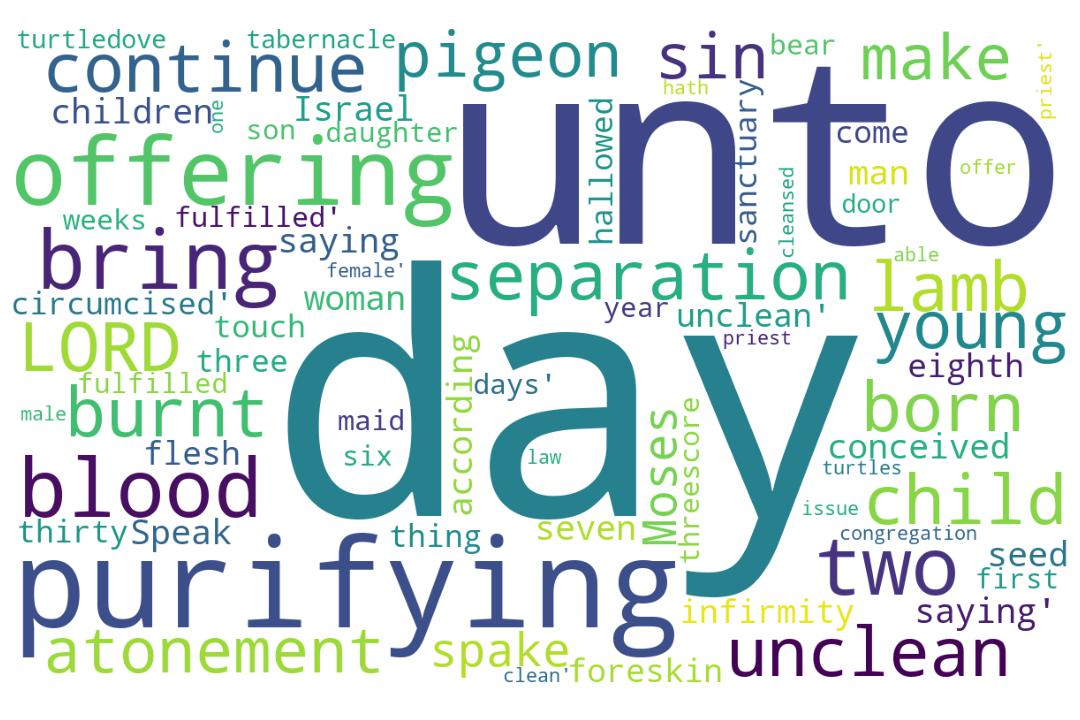
\includegraphics[width=\linewidth]{03OT-Leviticus/Leviticus12-WordCloud.jpg}
  \caption{Leviticus 12 Word Cloud}
  \label{fig:Leviticus 12 word Cloud}
\end{figure}

\marginpar{\scriptsize \centering \fcolorbox{bone}{lime}{\textbf{A POSTPARTUM BATH}}\\ (Leviticus 12:1--8) 
\begin{compactenum}[I.][8]
    \item \textbf{Time Periods} 
    \begin{compactenum}[A.][7]
		\item seven days  \index[scripture]{Leviticus!Lev 12:02} (Lev 12:2)
		\item eighth day \index[scripture]{Leviticus!Lev 12:03} (Lev 12:3)
		\item three and thirty days \index[scripture]{Leviticus!Lev 12:04} (Lev 12:4)
		\item two weeks \index[scripture]{Leviticus!Lev 12:05} (Lev 12:5)
		\item threescore and six days \index[scripture]{Leviticus!Lev 12:05} (Lev 12:5)
		\item first year \index[scripture]{Leviticus!Lev 12:06} (Lev 12:6)
    \end{compactenum}
    \item A \textbf{Telling Proclamation} \index[scripture]{Leviticus!Lev 12:02} (Lev 12:2)
    \item \textbf{Total Purification}  \index[scripture]{Leviticus!Lev 12:04} (Lev 12:4)
    \item \textbf{Verboten Place}  \index[scripture]{Leviticus!Lev 12:04} (Lev 12:4)
    \item \textbf{Trusted Priest} \index[scripture]{Leviticus!Lev 12:06} (Lev 12:6)
    \item \textbf{Turtles \& Pigeons}  \index[scripture]{Leviticus!Lev 12:08} (Lev 12:8)
\end{compactenum} 
}

%%%%%%%%%%%%%%%%%%%%%%%%%%%%%%%%%%
%%%%%%%%%%%%%%%%%%%%%%%%%%%%%%%%%%
\footnote{\textcolor[cmyk]{0.99998,1,0,0}{\hyperlink{TOC}{Return to end of Table of Contents.}}}\footnote{\href{https://audiobible.com/bible/leviticus_12.html}{\textcolor[cmyk]{0.99998,1,0,0}{Leviticus 12 Audio}}}\textcolor[cmyk]{0.99998,1,0,0}{And the LORD spake unto Moses, saying,}
[2] \textcolor[cmyk]{0.99998,1,0,0}{Speak unto the children of Israel, saying, If a woman have conceived seed, and born a man child: then she \fcolorbox{bone}{bone}{shall} be unclean \fcolorbox{bone}{lime}{seven days}; according to the days of the separation for her infirmity \fcolorbox{bone}{bone}{shall} she be \fcolorbox{bone}{lime}{unclean}.}
[3] \textcolor[cmyk]{0.99998,1,0,0}{And in the \fcolorbox{bone}{lime}{eighth day} the flesh of his foreskin \fcolorbox{bone}{bone}{shall} be circumcised.}
[4] \textcolor[cmyk]{0.99998,1,0,0}{And she \fcolorbox{bone}{bone}{shall} then continue in the blood of her purifying \fcolorbox{bone}{lime}{three and thirty} days; she \fcolorbox{bone}{bone}{shall} touch no hallowed thing, \fcolorbox{bone}{lime}{nor come into} the sanctuary, until the days of her purifying be fulfilled.}
[5] \textcolor[cmyk]{0.99998,1,0,0}{But if she bear a maid child, then she \fcolorbox{bone}{bone}{shall} be unclean \fcolorbox{bone}{lime}{two weeks}, as in her separation: and she \fcolorbox{bone}{bone}{shall} continue in the blood of her purifying \fcolorbox{bone}{lime}{threescore and six days}.}
[6] \textcolor[cmyk]{0.99998,1,0,0}{And when the days of her purifying are fulfilled, for a son, or for a daughter, she \fcolorbox{bone}{bone}{shall} bring a lamb of the \fcolorbox{bone}{lime}{first year} for a burnt offering, and a young pigeon, or a turtledove, for a sin offering, unto the door of the tabernacle of the congregation, unto the \fcolorbox{bone}{lime}{priest}:}
[7] \textcolor[cmyk]{0.99998,1,0,0}{Who \fcolorbox{bone}{bone}{shall} offer it before the LORD, and make an atonement for her; and she \fcolorbox{bone}{bone}{shall} be cleansed from the issue of her blood. This \emph{is} the law for her that hath born a male or a female.}
[8] \textcolor[cmyk]{0.99998,1,0,0}{And if she be not able to bring a lamb, then she \fcolorbox{bone}{bone}{shall} bring two \fcolorbox{bone}{lime}{turtles}, or two young \fcolorbox{bone}{lime}{pigeons}; the one for the burnt offering, and the other for a sin offering: and the priest \fcolorbox{bone}{bone}{shall} make an atonement for her, and she \fcolorbox{bone}{bone}{shall} be clean.}
\index[NWIV]{7!Leviticus!Lev 12:1}\index[AWIP]{And!Leviticus!Lev 12:1}\index[AWIP]{the!Leviticus!Lev 12:1}\index[AWIP]{LORD!Leviticus!Lev 12:1}\index[AWIP]{spake!Leviticus!Lev 12:1}\index[AWIP]{unto!Leviticus!Lev 12:1}\index[AWIP]{Moses!Leviticus!Lev 12:1}\index[AWIP]{saying!Leviticus!Lev 12:1}

\index[NWIV]{39!Leviticus!Lev 12:2}\index[AWIP]{Speak!Leviticus!Lev 12:2}\index[AWIP]{unto!Leviticus!Lev 12:2}\index[AWIP]{the!Leviticus!Lev 12:2}\index[AWIP]{the!Leviticus!Lev 12:2 (2)}\index[AWIP]{the!Leviticus!Lev 12:2 (3)}\index[AWIP]{children!Leviticus!Lev 12:2}\index[AWIP]{of!Leviticus!Lev 12:2}\index[AWIP]{of!Leviticus!Lev 12:2 (2)}\index[AWIP]{Israel!Leviticus!Lev 12:2}\index[AWIP]{saying!Leviticus!Lev 12:2}\index[AWIP]{If!Leviticus!Lev 12:2}\index[AWIP]{a!Leviticus!Lev 12:2}\index[AWIP]{a!Leviticus!Lev 12:2 (2)}\index[AWIP]{woman!Leviticus!Lev 12:2}\index[AWIP]{have!Leviticus!Lev 12:2}\index[AWIP]{conceived!Leviticus!Lev 12:2}\index[AWIP]{seed!Leviticus!Lev 12:2}\index[AWIP]{and!Leviticus!Lev 12:2}\index[AWIP]{born!Leviticus!Lev 12:2}\index[AWIP]{man!Leviticus!Lev 12:2}\index[AWIP]{child!Leviticus!Lev 12:2}\index[AWIP]{then!Leviticus!Lev 12:2}\index[AWIP]{she!Leviticus!Lev 12:2}\index[AWIP]{she!Leviticus!Lev 12:2 (2)}\index[AWIP]{shall!Leviticus!Lev 12:2}\index[AWIP]{shall!Leviticus!Lev 12:2 (2)}\index[AWIP]{be!Leviticus!Lev 12:2}\index[AWIP]{be!Leviticus!Lev 12:2 (2)}\index[AWIP]{unclean!Leviticus!Lev 12:2}\index[AWIP]{unclean!Leviticus!Lev 12:2 (2)}\index[AWIP]{seven!Leviticus!Lev 12:2}\index[AWIP]{days!Leviticus!Lev 12:2}\index[AWIP]{days!Leviticus!Lev 12:2 (2)}\index[AWIP]{according!Leviticus!Lev 12:2}\index[AWIP]{to!Leviticus!Lev 12:2}\index[AWIP]{separation!Leviticus!Lev 12:2}\index[AWIP]{for!Leviticus!Lev 12:2}\index[AWIP]{her!Leviticus!Lev 12:2}\index[AWIP]{infirmity!Leviticus!Lev 12:2}

\index[NWIV]{13!Leviticus!Lev 12:3}\index[AWIP]{And!Leviticus!Lev 12:3}\index[AWIP]{in!Leviticus!Lev 12:3}\index[AWIP]{the!Leviticus!Lev 12:3}\index[AWIP]{the!Leviticus!Lev 12:3 (2)}\index[AWIP]{eighth!Leviticus!Lev 12:3}\index[AWIP]{day!Leviticus!Lev 12:3}\index[AWIP]{flesh!Leviticus!Lev 12:3}\index[AWIP]{of!Leviticus!Lev 12:3}\index[AWIP]{his!Leviticus!Lev 12:3}\index[AWIP]{foreskin!Leviticus!Lev 12:3}\index[AWIP]{shall!Leviticus!Lev 12:3}\index[AWIP]{be!Leviticus!Lev 12:3}\index[AWIP]{circumcised!Leviticus!Lev 12:3}

\index[NWIV]{34!Leviticus!Lev 12:4}\index[AWIP]{And!Leviticus!Lev 12:4}\index[AWIP]{she!Leviticus!Lev 12:4}\index[AWIP]{she!Leviticus!Lev 12:4 (2)}\index[AWIP]{shall!Leviticus!Lev 12:4}\index[AWIP]{shall!Leviticus!Lev 12:4 (2)}\index[AWIP]{then!Leviticus!Lev 12:4}\index[AWIP]{continue!Leviticus!Lev 12:4}\index[AWIP]{in!Leviticus!Lev 12:4}\index[AWIP]{the!Leviticus!Lev 12:4}\index[AWIP]{the!Leviticus!Lev 12:4 (2)}\index[AWIP]{the!Leviticus!Lev 12:4 (3)}\index[AWIP]{blood!Leviticus!Lev 12:4}\index[AWIP]{of!Leviticus!Lev 12:4}\index[AWIP]{of!Leviticus!Lev 12:4 (2)}\index[AWIP]{her!Leviticus!Lev 12:4}\index[AWIP]{her!Leviticus!Lev 12:4 (2)}\index[AWIP]{purifying!Leviticus!Lev 12:4}\index[AWIP]{purifying!Leviticus!Lev 12:4 (2)}\index[AWIP]{three!Leviticus!Lev 12:4}\index[AWIP]{and!Leviticus!Lev 12:4}\index[AWIP]{thirty!Leviticus!Lev 12:4}\index[AWIP]{days!Leviticus!Lev 12:4}\index[AWIP]{days!Leviticus!Lev 12:4 (2)}\index[AWIP]{touch!Leviticus!Lev 12:4}\index[AWIP]{no!Leviticus!Lev 12:4}\index[AWIP]{hallowed!Leviticus!Lev 12:4}\index[AWIP]{thing!Leviticus!Lev 12:4}\index[AWIP]{nor!Leviticus!Lev 12:4}\index[AWIP]{come!Leviticus!Lev 12:4}\index[AWIP]{into!Leviticus!Lev 12:4}\index[AWIP]{sanctuary!Leviticus!Lev 12:4}\index[AWIP]{until!Leviticus!Lev 12:4}\index[AWIP]{be!Leviticus!Lev 12:4}\index[AWIP]{fulfilled!Leviticus!Lev 12:4}

\index[NWIV]{32!Leviticus!Lev 12:5}\index[AWIP]{But!Leviticus!Lev 12:5}\index[AWIP]{if!Leviticus!Lev 12:5}\index[AWIP]{she!Leviticus!Lev 12:5}\index[AWIP]{she!Leviticus!Lev 12:5 (2)}\index[AWIP]{she!Leviticus!Lev 12:5 (3)}\index[AWIP]{bear!Leviticus!Lev 12:5}\index[AWIP]{a!Leviticus!Lev 12:5}\index[AWIP]{maid!Leviticus!Lev 12:5}\index[AWIP]{child!Leviticus!Lev 12:5}\index[AWIP]{then!Leviticus!Lev 12:5}\index[AWIP]{shall!Leviticus!Lev 12:5}\index[AWIP]{shall!Leviticus!Lev 12:5 (2)}\index[AWIP]{be!Leviticus!Lev 12:5}\index[AWIP]{unclean!Leviticus!Lev 12:5}\index[AWIP]{two!Leviticus!Lev 12:5}\index[AWIP]{weeks!Leviticus!Lev 12:5}\index[AWIP]{as!Leviticus!Lev 12:5}\index[AWIP]{in!Leviticus!Lev 12:5}\index[AWIP]{in!Leviticus!Lev 12:5 (2)}\index[AWIP]{her!Leviticus!Lev 12:5}\index[AWIP]{her!Leviticus!Lev 12:5 (2)}\index[AWIP]{separation!Leviticus!Lev 12:5}\index[AWIP]{and!Leviticus!Lev 12:5}\index[AWIP]{and!Leviticus!Lev 12:5 (2)}\index[AWIP]{continue!Leviticus!Lev 12:5}\index[AWIP]{the!Leviticus!Lev 12:5}\index[AWIP]{blood!Leviticus!Lev 12:5}\index[AWIP]{of!Leviticus!Lev 12:5}\index[AWIP]{purifying!Leviticus!Lev 12:5}\index[AWIP]{threescore!Leviticus!Lev 12:5}\index[AWIP]{six!Leviticus!Lev 12:5}\index[AWIP]{days!Leviticus!Lev 12:5}

\index[NWIV]{52!Leviticus!Lev 12:6}\index[AWIP]{And!Leviticus!Lev 12:6}\index[AWIP]{when!Leviticus!Lev 12:6}\index[AWIP]{the!Leviticus!Lev 12:6}\index[AWIP]{the!Leviticus!Lev 12:6 (2)}\index[AWIP]{the!Leviticus!Lev 12:6 (3)}\index[AWIP]{the!Leviticus!Lev 12:6 (4)}\index[AWIP]{the!Leviticus!Lev 12:6 (5)}\index[AWIP]{the!Leviticus!Lev 12:6 (6)}\index[AWIP]{days!Leviticus!Lev 12:6}\index[AWIP]{of!Leviticus!Lev 12:6}\index[AWIP]{of!Leviticus!Lev 12:6 (2)}\index[AWIP]{of!Leviticus!Lev 12:6 (3)}\index[AWIP]{of!Leviticus!Lev 12:6 (4)}\index[AWIP]{her!Leviticus!Lev 12:6}\index[AWIP]{purifying!Leviticus!Lev 12:6}\index[AWIP]{are!Leviticus!Lev 12:6}\index[AWIP]{fulfilled!Leviticus!Lev 12:6}\index[AWIP]{for!Leviticus!Lev 12:6}\index[AWIP]{for!Leviticus!Lev 12:6 (2)}\index[AWIP]{for!Leviticus!Lev 12:6 (3)}\index[AWIP]{for!Leviticus!Lev 12:6 (4)}\index[AWIP]{a!Leviticus!Lev 12:6}\index[AWIP]{a!Leviticus!Lev 12:6 (2)}\index[AWIP]{a!Leviticus!Lev 12:6 (3)}\index[AWIP]{a!Leviticus!Lev 12:6 (4)}\index[AWIP]{a!Leviticus!Lev 12:6 (5)}\index[AWIP]{a!Leviticus!Lev 12:6 (6)}\index[AWIP]{a!Leviticus!Lev 12:6 (7)}\index[AWIP]{son!Leviticus!Lev 12:6}\index[AWIP]{or!Leviticus!Lev 12:6}\index[AWIP]{or!Leviticus!Lev 12:6 (2)}\index[AWIP]{daughter!Leviticus!Lev 12:6}\index[AWIP]{she!Leviticus!Lev 12:6}\index[AWIP]{shall!Leviticus!Lev 12:6}\index[AWIP]{bring!Leviticus!Lev 12:6}\index[AWIP]{lamb!Leviticus!Lev 12:6}\index[AWIP]{first!Leviticus!Lev 12:6}\index[AWIP]{year!Leviticus!Lev 12:6}\index[AWIP]{burnt!Leviticus!Lev 12:6}\index[AWIP]{offering!Leviticus!Lev 12:6}\index[AWIP]{offering!Leviticus!Lev 12:6 (2)}\index[AWIP]{and!Leviticus!Lev 12:6}\index[AWIP]{young!Leviticus!Lev 12:6}\index[AWIP]{pigeon!Leviticus!Lev 12:6}\index[AWIP]{turtledove!Leviticus!Lev 12:6}\index[AWIP]{sin!Leviticus!Lev 12:6}\index[AWIP]{unto!Leviticus!Lev 12:6}\index[AWIP]{unto!Leviticus!Lev 12:6 (2)}\index[AWIP]{door!Leviticus!Lev 12:6}\index[AWIP]{tabernacle!Leviticus!Lev 12:6}\index[AWIP]{congregation!Leviticus!Lev 12:6}\index[AWIP]{priest!Leviticus!Lev 12:6}

\index[NWIV]{38!Leviticus!Lev 12:7}\index[AWIP]{Who!Leviticus!Lev 12:7}\index[AWIP]{shall!Leviticus!Lev 12:7}\index[AWIP]{shall!Leviticus!Lev 12:7 (2)}\index[AWIP]{offer!Leviticus!Lev 12:7}\index[AWIP]{it!Leviticus!Lev 12:7}\index[AWIP]{before!Leviticus!Lev 12:7}\index[AWIP]{the!Leviticus!Lev 12:7}\index[AWIP]{the!Leviticus!Lev 12:7 (2)}\index[AWIP]{the!Leviticus!Lev 12:7 (3)}\index[AWIP]{LORD!Leviticus!Lev 12:7}\index[AWIP]{and!Leviticus!Lev 12:7}\index[AWIP]{and!Leviticus!Lev 12:7 (2)}\index[AWIP]{make!Leviticus!Lev 12:7}\index[AWIP]{an!Leviticus!Lev 12:7}\index[AWIP]{atonement!Leviticus!Lev 12:7}\index[AWIP]{for!Leviticus!Lev 12:7}\index[AWIP]{for!Leviticus!Lev 12:7 (2)}\index[AWIP]{her!Leviticus!Lev 12:7}\index[AWIP]{her!Leviticus!Lev 12:7 (2)}\index[AWIP]{her!Leviticus!Lev 12:7 (3)}\index[AWIP]{she!Leviticus!Lev 12:7}\index[AWIP]{be!Leviticus!Lev 12:7}\index[AWIP]{cleansed!Leviticus!Lev 12:7}\index[AWIP]{from!Leviticus!Lev 12:7}\index[AWIP]{issue!Leviticus!Lev 12:7}\index[AWIP]{of!Leviticus!Lev 12:7}\index[AWIP]{blood!Leviticus!Lev 12:7}\index[AWIP]{This!Leviticus!Lev 12:7}\index[AWIP]{\emph{is}!Leviticus!Lev 12:7}\index[AWIP]{law!Leviticus!Lev 12:7}\index[AWIP]{that!Leviticus!Lev 12:7}\index[AWIP]{hath!Leviticus!Lev 12:7}\index[AWIP]{born!Leviticus!Lev 12:7}\index[AWIP]{a!Leviticus!Lev 12:7}\index[AWIP]{a!Leviticus!Lev 12:7 (2)}\index[AWIP]{male!Leviticus!Lev 12:7}\index[AWIP]{or!Leviticus!Lev 12:7}\index[AWIP]{female!Leviticus!Lev 12:7}\index[AWIP]{\emph{is}!Leviticus!Lev 12:7}

\index[NWIV]{47!Leviticus!Lev 12:8}\index[AWIP]{And!Leviticus!Lev 12:8}\index[AWIP]{if!Leviticus!Lev 12:8}\index[AWIP]{she!Leviticus!Lev 12:8}\index[AWIP]{she!Leviticus!Lev 12:8 (2)}\index[AWIP]{she!Leviticus!Lev 12:8 (3)}\index[AWIP]{be!Leviticus!Lev 12:8}\index[AWIP]{be!Leviticus!Lev 12:8 (2)}\index[AWIP]{not!Leviticus!Lev 12:8}\index[AWIP]{able!Leviticus!Lev 12:8}\index[AWIP]{to!Leviticus!Lev 12:8}\index[AWIP]{bring!Leviticus!Lev 12:8}\index[AWIP]{bring!Leviticus!Lev 12:8 (2)}\index[AWIP]{a!Leviticus!Lev 12:8}\index[AWIP]{a!Leviticus!Lev 12:8 (2)}\index[AWIP]{lamb!Leviticus!Lev 12:8}\index[AWIP]{then!Leviticus!Lev 12:8}\index[AWIP]{shall!Leviticus!Lev 12:8}\index[AWIP]{shall!Leviticus!Lev 12:8 (2)}\index[AWIP]{shall!Leviticus!Lev 12:8 (3)}\index[AWIP]{two!Leviticus!Lev 12:8}\index[AWIP]{two!Leviticus!Lev 12:8 (2)}\index[AWIP]{turtles!Leviticus!Lev 12:8}\index[AWIP]{or!Leviticus!Lev 12:8}\index[AWIP]{young!Leviticus!Lev 12:8}\index[AWIP]{pigeons!Leviticus!Lev 12:8}\index[AWIP]{the!Leviticus!Lev 12:8}\index[AWIP]{the!Leviticus!Lev 12:8 (2)}\index[AWIP]{the!Leviticus!Lev 12:8 (3)}\index[AWIP]{the!Leviticus!Lev 12:8 (4)}\index[AWIP]{one!Leviticus!Lev 12:8}\index[AWIP]{for!Leviticus!Lev 12:8}\index[AWIP]{for!Leviticus!Lev 12:8 (2)}\index[AWIP]{for!Leviticus!Lev 12:8 (3)}\index[AWIP]{burnt!Leviticus!Lev 12:8}\index[AWIP]{offering!Leviticus!Lev 12:8}\index[AWIP]{offering!Leviticus!Lev 12:8 (2)}\index[AWIP]{and!Leviticus!Lev 12:8}\index[AWIP]{and!Leviticus!Lev 12:8 (2)}\index[AWIP]{and!Leviticus!Lev 12:8 (3)}\index[AWIP]{other!Leviticus!Lev 12:8}\index[AWIP]{sin!Leviticus!Lev 12:8}\index[AWIP]{priest!Leviticus!Lev 12:8}\index[AWIP]{make!Leviticus!Lev 12:8}\index[AWIP]{an!Leviticus!Lev 12:8}\index[AWIP]{atonement!Leviticus!Lev 12:8}\index[AWIP]{her!Leviticus!Lev 12:8}\index[AWIP]{clean!Leviticus!Lev 12:8}


\section{Leviticus  12 Outlines}

\subsection{My Outlines}

\subsubsection{A Postpartum Bath}
\index[speaker]{Keith Anthony!Leviticus 12 (A Postpartum Bath)}
\index[series]{Leviticus (Keith Anthony)!Leviticus 12 (A Postpartum Bath)}
\index[date]{2017/02/01!Leviticus 12 (A Postpartum Bath) (Keith Anthony)}
%\textbf{Introduction: }He was
\begin{compactenum}[I.][7]
    \item \textbf{Time Periods} 
    \begin{compactenum}[A.][7]
		\item seven days  \index[scripture]{Leviticus!Lev 12:02} (Lev 12:2)
		\item eighth day \index[scripture]{Leviticus!Lev 12:03} (Lev 12:3)
		\item three and thirty days \index[scripture]{Leviticus!Lev 12:04} (Lev 12:4)
		\item two weeks \index[scripture]{Leviticus!Lev 12:05} (Lev 12:5)
		\item threescore and six days \index[scripture]{Leviticus!Lev 12:05} (Lev 12:5)
		\item first year \index[scripture]{Leviticus!Lev 12:06} (Lev 12:6)
    \end{compactenum}
    \item A \textbf{Telling Proclamation} \index[scripture]{Leviticus!Lev 12:02} (Lev 12:2)
    \item \textbf{Total Purification}  \index[scripture]{Leviticus!Lev 12:04} (Lev 12:4)
    \item \textbf{Verboten Place}  \index[scripture]{Leviticus!Lev 12:04} (Lev 12:4)
    \item \textbf{Trusted Priest} \index[scripture]{Leviticus!Lev 12:06} (Lev 12:6)
    \item \textbf{Turtles \& Pigeons}  \index[scripture]{Leviticus!Lev 12:08} (Lev 12:8)
\end{compactenum}

\subsection{Outlines from Others}
\section{Leviticus 12 Comments}

\subsection{Numeric Nuggets}
\textbf{66: } The phrase ``threescore and six'' is found in verse 5.  This is a suspicious phase, used also when counting the number of souls that came of Jacob into Egypt in Genesis 46:26.\footnote{\textbf{Genesis 46:26} -  All the souls that came with Jacob into Egypt, which came out of his loins, besides Jacob’s sons’ wives, all the souls were threescore and six;} The phrase is also a part of the ``six hundred threescore and six'' phrase found in 1 Kings 10:14, 2 Chronicles 9:13, and Revelation 13:18.\\
\noindent \textbf{13: } One verse in Leviticus 12 has 13 words, Leviticus 12:12. The word ``shall'' is found 13 times in the chapter.



\chapter{Psalm 35}

\begin{figure}
  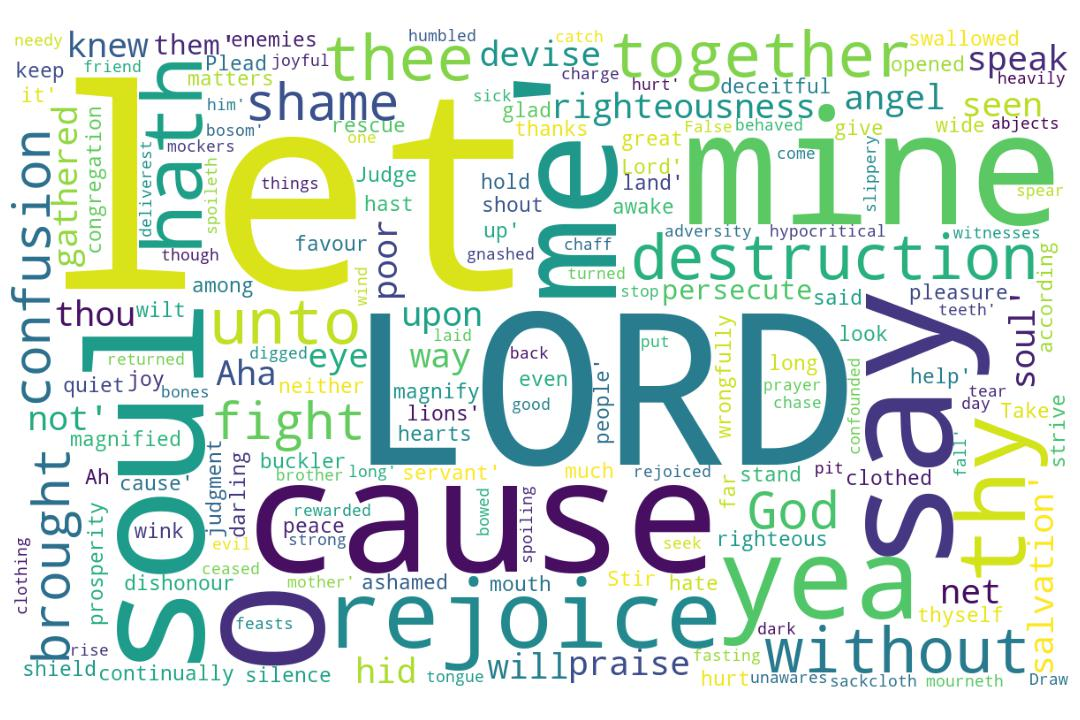
\includegraphics[width=\linewidth]{19OT-Psalms/Psalm35-WordCloud.jpg}
  \caption{Psalm 35 Word Cloud}
  \label{fig:Psalm 35 word Cloud}
\end{figure}

\marginpar{\scriptsize \centering \fcolorbox{bone}{lime}{\textbf{A HEARTFELT CRY}}\\ (Psalm 35:1--28) 
\begin{compactenum}[I.][8]
    \item A \textbf{Distinct  Petition} \index[scripture]{Psalms!Psa 035:24} (Psa 35:24)  (for enemies $\hdots$)
    \begin{compactenum}[A.][7]
		\item To be Confounded \index[scripture]{Psalms!Psa 035:04} (Psa 35:4)
		\item To be Confused \index[scripture]{Psalms!Psa 035:04}\index[scripture]{Psalms!Psa 035:26} (Psa 35:4, 26)
		\item To Become Chaff \index[scripture]{Psalms!Psa 035:05} (Psa 35:5)
		\item To be Chased \index[scripture]{Psalms!Psa 035:05} (Psa 35:5)
		\item To be Consumed \index[scripture]{Psalms!Psa 035:08} (Psa 35:8)
		\item To be Clothed in Shame \index[scripture]{Psalms!Psa 035:25} (Psa 35:25)
		\item To be Conquered \index[scripture]{Psalms!Psa 035:28} (Psa 35:28)
    \end{compactenum}
    \item A \textbf{Dangerous Prayer} \index[scripture]{Psalms!Psa 035:24} (Psa 35:24)
    \item A \textbf{Definite Promise} \index[scripture]{Psalms!Psa 035:28} (Psa 35:28)
\end{compactenum} }

\marginpar{\scriptsize \centering \fcolorbox{bone}{yellow}{\textbf{HELP, PLEASE!}}\\ (Psalm 35:1--28) 
\begin{compactenum}[I.][8]

    \item  The \textbf{Asking} \index[scripture]{Psalms!Psa 035:01} (Psa 35:1)  
    \item  \textbf{Admiration} \index[scripture]{Psalms!Psa 035:10} (Psa 35:10)  
    \item  \textbf{Adversity} \index[scripture]{Psalms!Psa 035:15} (Psa 35:15)  
    \item  \textbf{Abjects} \index[scripture]{Psalms!Psa 035:15} (Psa 35:15)  
    \item  \textbf{Adversaries} \index[scripture]{Psalms!Psa 035:15} (Psa 35:15)  
    \item  \textbf{Assembly} \index[scripture]{Psalms!Psa 035:18} (Psa 35:18)  
    \item  \textbf{Activation} \index[scripture]{Psalms!Psa 035:23} (Psa 35:23)  
    \item  \textbf{Acknowledgment} \index[scripture]{Psalms!Psa 035:27} (Psa 35:27)  
\end{compactenum} }

%%%%%%%%%%%%%%%%%%%%%%%%%%%%%%%%%%%%%%%%%%%%%%
%%%%%%%%%%%%%%%%%%%%%%%%%%%%%%%%%%%%%%%%%%%%%%
\footnote{\textcolor[cmyk]{0.99998,1,0,0}{\hyperlink{TOC}{Return to end of Table of Contents.}}}\footnote{\href{https://www.audioverse.org/english/audiobibles/books/ENGKJV/O/Ps/1}{\textcolor[cmyk]{0.99998,1,0,0}{Psalms Audio}}}\textcolor[cmyk]{0.99998,1,0,0}{Plead \emph{my} \emph{cause}, O LORD, with them that strive with me: fight against them that fight against me.}\marginpar{\scriptsize \textcolor[rgb]{0.00,0.545,0.269}{$\rightarrow$(1) Strife [1], (2) Shield [2], (3) Spear [3], (4) Salvation [3], (5) Shame [4], (6) Slipping [6], (7) Spoiling [10].}}
[2] \textcolor[cmyk]{0.99998,1,0,0}{Take hold of shield and buckler, and stand up for mine help.}
[3] \textcolor[cmyk]{0.99998,1,0,0}{Draw out also the spear, and stop \emph{the} \emph{way} against them that persecute me: say unto my soul, I \emph{am} thy salvation.}
[4] \textcolor[cmyk]{0.99998,1,0,0}{Let them be \fcolorbox{bone}{lime}{confounded} and put to shame that seek after my soul: let them be turned back and brought to \fcolorbox{bone}{lime}{confusion} that devise my hurt.}
[5] \textcolor[cmyk]{0.99998,1,0,0}{Let them be as \fcolorbox{bone}{lime}{chaff} before the wind: and let the angel of the LORD \fcolorbox{bone}{lime}{chase} \emph{them}.}
[6] \textcolor[cmyk]{0.99998,1,0,0}{Let their way be dark and slippery: and let the angel of the LORD persecute them.}
[7] \textcolor[cmyk]{0.99998,1,0,0}{For without cause have they hid for me their net \emph{in} a pit, \emph{which} without cause they have digged for my soul.}
[8] \textcolor[cmyk]{0.99998,1,0,0}{Let \fcolorbox{bone}{lime}{destruction} come upon him at unawares; and let his net that he hath hid catch himself: into that very destruction let him fall.}
[9] \textcolor[cmyk]{0.99998,1,0,0}{And my soul shall be joyful in the LORD: it shall rejoice in his salvation.}
[10] \textcolor[cmyk]{0.99998,1,0,0}{All my bones shall say, LORD, who \emph{is} like unto thee, which deliverest the poor from him that is too strong for him, yea, the poor and the needy from him that spoileth him?}
[11] \textcolor[cmyk]{0.99998,1,0,0}{False witnesses did rise up; they laid to my charge \emph{things} that I knew not.}
[12] \textcolor[cmyk]{0.99998,1,0,0}{They rewarded me evil for good \emph{to} the spoiling of my soul.}
[13] \textcolor[cmyk]{0.99998,1,0,0}{But as for me, when they were sick, my clothing \emph{was} sackcloth: I humbled my soul with fasting; and my prayer returned into mine own bosom.}
[14] \textcolor[cmyk]{0.99998,1,0,0}{I behaved myself as though \emph{he} \emph{had} \emph{been} my friend \emph{or} brother: I bowed down heavily, as one that mourneth \emph{for} \emph{his} mother.}
[15] \textcolor[cmyk]{0.99998,1,0,0}{But in mine adversity they rejoiced, and gathered themselves together: \emph{yea}, the abjects gathered themselves together against me, and I knew \emph{it} not; they did tear \emph{me}, and ceased not:}
[16] \textcolor[cmyk]{0.99998,1,0,0}{With hypocritical mockers in feasts, they gnashed upon me with their teeth.}
[17] \textcolor[cmyk]{0.99998,1,0,0}{Lord, how long wilt thou look on? rescue my soul from their destructions, my darling from the lions.}
[18] \textcolor[cmyk]{0.99998,1,0,0}{I will give thee thanks in the great congregation: I will praise thee among much people.}
[19] \textcolor[cmyk]{0.99998,1,0,0}{Let not them that are mine enemies wrongfully rejoice over me: \emph{neither} let them wink with the eye that hate me without a cause.}
[20] \textcolor[cmyk]{0.99998,1,0,0}{For they speak not peace: but they devise deceitful matters against \emph{them} \emph{that} \emph{are} quiet in the land.}
[21] \textcolor[cmyk]{0.99998,1,0,0}{Yea, they opened their mouth wide against me, \emph{and} said, Aha, aha, our eye hath seen \emph{it}.}
[22] \textcolor[cmyk]{0.99998,1,0,0}{\emph{This} thou hast seen, O LORD: keep not silence: O Lord, be not far from me.}
[23] \textcolor[cmyk]{0.99998,1,0,0}{Stir up thyself, and awake to my judgment, \emph{even} unto my cause, my God and my Lord.}
[24] \textcolor[cmyk]{0.99998,1,0,0}{\fcolorbox{bone}{lime}{Judge me}, O LORD my God, according to thy righteousness; and let them not rejoice over me.}
[25] \textcolor[cmyk]{0.99998,1,0,0}{Let them not say in their hearts, Ah, so would we have it: let them not say, We have swallowed him up.}
[26] \textcolor[cmyk]{0.99998,1,0,0}{Let them be ashamed and brought to confusion together that rejoice at mine hurt: let them be clothed with shame and dishonour that magnify \emph{themselves} against me.}
[27] \textcolor[cmyk]{0.99998,1,0,0}{Let them shout for joy, and be glad, that favour my righteous cause: yea, let them say continually, Let the LORD be magnified, which hath pleasure in the prosperity of his servant.}
[28] \textcolor[cmyk]{0.99998,1,0,0}{And my tongue \fcolorbox{bone}{lime}{shall speak} of thy righteousness \emph{and} of thy praise all the day long.}



\index[NWIV]{18!Psalms!Psa 35:1}\index[AWIP]{Plead!Psalms!Psa 35:1}\index[AWIP]{\emph{my}!Psalms!Psa 35:1}\index[AWIP]{\emph{cause}!Psalms!Psa 35:1}\index[AWIP]{O!Psalms!Psa 35:1}\index[AWIP]{LORD!Psalms!Psa 35:1}\index[AWIP]{with!Psalms!Psa 35:1}\index[AWIP]{with!Psalms!Psa 35:1 (2)}\index[AWIP]{them!Psalms!Psa 35:1}\index[AWIP]{them!Psalms!Psa 35:1 (2)}\index[AWIP]{that!Psalms!Psa 35:1}\index[AWIP]{that!Psalms!Psa 35:1 (2)}\index[AWIP]{strive!Psalms!Psa 35:1}\index[AWIP]{me!Psalms!Psa 35:1}\index[AWIP]{me!Psalms!Psa 35:1 (2)}\index[AWIP]{fight!Psalms!Psa 35:1}\index[AWIP]{fight!Psalms!Psa 35:1 (2)}\index[AWIP]{against!Psalms!Psa 35:1}\index[AWIP]{against!Psalms!Psa 35:1 (2)}\index[AWIP]{\emph{my}!Psalms!Psa 35:1}\index[AWIP]{\emph{cause}!Psalms!Psa 35:1}

\index[NWIV]{12!Psalms!Psa 35:2}\index[AWIP]{Take!Psalms!Psa 35:2}\index[AWIP]{hold!Psalms!Psa 35:2}\index[AWIP]{of!Psalms!Psa 35:2}\index[AWIP]{shield!Psalms!Psa 35:2}\index[AWIP]{and!Psalms!Psa 35:2}\index[AWIP]{and!Psalms!Psa 35:2 (2)}\index[AWIP]{buckler!Psalms!Psa 35:2}\index[AWIP]{stand!Psalms!Psa 35:2}\index[AWIP]{up!Psalms!Psa 35:2}\index[AWIP]{for!Psalms!Psa 35:2}\index[AWIP]{mine!Psalms!Psa 35:2}\index[AWIP]{help!Psalms!Psa 35:2}

\index[NWIV]{22!Psalms!Psa 35:3}\index[AWIP]{Draw!Psalms!Psa 35:3}\index[AWIP]{out!Psalms!Psa 35:3}\index[AWIP]{also!Psalms!Psa 35:3}\index[AWIP]{the!Psalms!Psa 35:3}\index[AWIP]{spear!Psalms!Psa 35:3}\index[AWIP]{and!Psalms!Psa 35:3}\index[AWIP]{stop!Psalms!Psa 35:3}\index[AWIP]{\emph{the}!Psalms!Psa 35:3}\index[AWIP]{\emph{way}!Psalms!Psa 35:3}\index[AWIP]{against!Psalms!Psa 35:3}\index[AWIP]{them!Psalms!Psa 35:3}\index[AWIP]{that!Psalms!Psa 35:3}\index[AWIP]{persecute!Psalms!Psa 35:3}\index[AWIP]{me!Psalms!Psa 35:3}\index[AWIP]{say!Psalms!Psa 35:3}\index[AWIP]{unto!Psalms!Psa 35:3}\index[AWIP]{my!Psalms!Psa 35:3}\index[AWIP]{soul!Psalms!Psa 35:3}\index[AWIP]{I!Psalms!Psa 35:3}\index[AWIP]{\emph{am}!Psalms!Psa 35:3}\index[AWIP]{thy!Psalms!Psa 35:3}\index[AWIP]{salvation!Psalms!Psa 35:3}\index[AWIP]{\emph{the}!Psalms!Psa 35:3}\index[AWIP]{\emph{way}!Psalms!Psa 35:3}\index[AWIP]{\emph{am}!Psalms!Psa 35:3}

\index[NWIV]{26!Psalms!Psa 35:4}\index[AWIP]{Let!Psalms!Psa 35:4}\index[AWIP]{them!Psalms!Psa 35:4}\index[AWIP]{them!Psalms!Psa 35:4 (2)}\index[AWIP]{be!Psalms!Psa 35:4}\index[AWIP]{be!Psalms!Psa 35:4 (2)}\index[AWIP]{confounded!Psalms!Psa 35:4}\index[AWIP]{and!Psalms!Psa 35:4}\index[AWIP]{and!Psalms!Psa 35:4 (2)}\index[AWIP]{put!Psalms!Psa 35:4}\index[AWIP]{to!Psalms!Psa 35:4}\index[AWIP]{to!Psalms!Psa 35:4 (2)}\index[AWIP]{shame!Psalms!Psa 35:4}\index[AWIP]{that!Psalms!Psa 35:4}\index[AWIP]{that!Psalms!Psa 35:4 (2)}\index[AWIP]{seek!Psalms!Psa 35:4}\index[AWIP]{after!Psalms!Psa 35:4}\index[AWIP]{my!Psalms!Psa 35:4}\index[AWIP]{my!Psalms!Psa 35:4 (2)}\index[AWIP]{soul!Psalms!Psa 35:4}\index[AWIP]{let!Psalms!Psa 35:4}\index[AWIP]{turned!Psalms!Psa 35:4}\index[AWIP]{back!Psalms!Psa 35:4}\index[AWIP]{brought!Psalms!Psa 35:4}\index[AWIP]{confusion!Psalms!Psa 35:4}\index[AWIP]{devise!Psalms!Psa 35:4}\index[AWIP]{hurt!Psalms!Psa 35:4}

\index[NWIV]{17!Psalms!Psa 35:5}\index[AWIP]{Let!Psalms!Psa 35:5}\index[AWIP]{them!Psalms!Psa 35:5}\index[AWIP]{be!Psalms!Psa 35:5}\index[AWIP]{as!Psalms!Psa 35:5}\index[AWIP]{chaff!Psalms!Psa 35:5}\index[AWIP]{before!Psalms!Psa 35:5}\index[AWIP]{the!Psalms!Psa 35:5}\index[AWIP]{the!Psalms!Psa 35:5 (2)}\index[AWIP]{the!Psalms!Psa 35:5 (3)}\index[AWIP]{wind!Psalms!Psa 35:5}\index[AWIP]{and!Psalms!Psa 35:5}\index[AWIP]{let!Psalms!Psa 35:5}\index[AWIP]{angel!Psalms!Psa 35:5}\index[AWIP]{of!Psalms!Psa 35:5}\index[AWIP]{LORD!Psalms!Psa 35:5}\index[AWIP]{chase!Psalms!Psa 35:5}\index[AWIP]{\emph{them}!Psalms!Psa 35:5}\index[AWIP]{\emph{them}!Psalms!Psa 35:5}

\index[NWIV]{16!Psalms!Psa 35:6}\index[AWIP]{Let!Psalms!Psa 35:6}\index[AWIP]{their!Psalms!Psa 35:6}\index[AWIP]{way!Psalms!Psa 35:6}\index[AWIP]{be!Psalms!Psa 35:6}\index[AWIP]{dark!Psalms!Psa 35:6}\index[AWIP]{and!Psalms!Psa 35:6}\index[AWIP]{and!Psalms!Psa 35:6 (2)}\index[AWIP]{slippery!Psalms!Psa 35:6}\index[AWIP]{let!Psalms!Psa 35:6}\index[AWIP]{the!Psalms!Psa 35:6}\index[AWIP]{the!Psalms!Psa 35:6 (2)}\index[AWIP]{angel!Psalms!Psa 35:6}\index[AWIP]{of!Psalms!Psa 35:6}\index[AWIP]{LORD!Psalms!Psa 35:6}\index[AWIP]{persecute!Psalms!Psa 35:6}\index[AWIP]{them!Psalms!Psa 35:6}

\index[NWIV]{22!Psalms!Psa 35:7}\index[AWIP]{For!Psalms!Psa 35:7}\index[AWIP]{without!Psalms!Psa 35:7}\index[AWIP]{without!Psalms!Psa 35:7 (2)}\index[AWIP]{cause!Psalms!Psa 35:7}\index[AWIP]{cause!Psalms!Psa 35:7 (2)}\index[AWIP]{have!Psalms!Psa 35:7}\index[AWIP]{have!Psalms!Psa 35:7 (2)}\index[AWIP]{they!Psalms!Psa 35:7}\index[AWIP]{they!Psalms!Psa 35:7 (2)}\index[AWIP]{hid!Psalms!Psa 35:7}\index[AWIP]{for!Psalms!Psa 35:7}\index[AWIP]{for!Psalms!Psa 35:7 (2)}\index[AWIP]{me!Psalms!Psa 35:7}\index[AWIP]{their!Psalms!Psa 35:7}\index[AWIP]{net!Psalms!Psa 35:7}\index[AWIP]{\emph{in}!Psalms!Psa 35:7}\index[AWIP]{a!Psalms!Psa 35:7}\index[AWIP]{pit!Psalms!Psa 35:7}\index[AWIP]{\emph{which}!Psalms!Psa 35:7}\index[AWIP]{digged!Psalms!Psa 35:7}\index[AWIP]{my!Psalms!Psa 35:7}\index[AWIP]{soul!Psalms!Psa 35:7}\index[AWIP]{\emph{in}!Psalms!Psa 35:7}\index[AWIP]{\emph{which}!Psalms!Psa 35:7}

\index[NWIV]{24!Psalms!Psa 35:8}\index[AWIP]{Let!Psalms!Psa 35:8}\index[AWIP]{destruction!Psalms!Psa 35:8}\index[AWIP]{destruction!Psalms!Psa 35:8 (2)}\index[AWIP]{come!Psalms!Psa 35:8}\index[AWIP]{upon!Psalms!Psa 35:8}\index[AWIP]{him!Psalms!Psa 35:8}\index[AWIP]{him!Psalms!Psa 35:8 (2)}\index[AWIP]{at!Psalms!Psa 35:8}\index[AWIP]{unawares!Psalms!Psa 35:8}\index[AWIP]{and!Psalms!Psa 35:8}\index[AWIP]{let!Psalms!Psa 35:8}\index[AWIP]{let!Psalms!Psa 35:8 (2)}\index[AWIP]{his!Psalms!Psa 35:8}\index[AWIP]{net!Psalms!Psa 35:8}\index[AWIP]{that!Psalms!Psa 35:8}\index[AWIP]{that!Psalms!Psa 35:8 (2)}\index[AWIP]{he!Psalms!Psa 35:8}\index[AWIP]{hath!Psalms!Psa 35:8}\index[AWIP]{hid!Psalms!Psa 35:8}\index[AWIP]{catch!Psalms!Psa 35:8}\index[AWIP]{himself!Psalms!Psa 35:8}\index[AWIP]{into!Psalms!Psa 35:8}\index[AWIP]{very!Psalms!Psa 35:8}\index[AWIP]{fall!Psalms!Psa 35:8}

\index[NWIV]{15!Psalms!Psa 35:9}\index[AWIP]{And!Psalms!Psa 35:9}\index[AWIP]{my!Psalms!Psa 35:9}\index[AWIP]{soul!Psalms!Psa 35:9}\index[AWIP]{shall!Psalms!Psa 35:9}\index[AWIP]{shall!Psalms!Psa 35:9 (2)}\index[AWIP]{be!Psalms!Psa 35:9}\index[AWIP]{joyful!Psalms!Psa 35:9}\index[AWIP]{in!Psalms!Psa 35:9}\index[AWIP]{in!Psalms!Psa 35:9 (2)}\index[AWIP]{the!Psalms!Psa 35:9}\index[AWIP]{LORD!Psalms!Psa 35:9}\index[AWIP]{it!Psalms!Psa 35:9}\index[AWIP]{rejoice!Psalms!Psa 35:9}\index[AWIP]{his!Psalms!Psa 35:9}\index[AWIP]{salvation!Psalms!Psa 35:9}

\index[NWIV]{34!Psalms!Psa 35:10}\index[AWIP]{All!Psalms!Psa 35:10}\index[AWIP]{my!Psalms!Psa 35:10}\index[AWIP]{bones!Psalms!Psa 35:10}\index[AWIP]{shall!Psalms!Psa 35:10}\index[AWIP]{say!Psalms!Psa 35:10}\index[AWIP]{LORD!Psalms!Psa 35:10}\index[AWIP]{who!Psalms!Psa 35:10}\index[AWIP]{\emph{is}!Psalms!Psa 35:10}\index[AWIP]{like!Psalms!Psa 35:10}\index[AWIP]{unto!Psalms!Psa 35:10}\index[AWIP]{thee!Psalms!Psa 35:10}\index[AWIP]{which!Psalms!Psa 35:10}\index[AWIP]{deliverest!Psalms!Psa 35:10}\index[AWIP]{the!Psalms!Psa 35:10}\index[AWIP]{the!Psalms!Psa 35:10 (2)}\index[AWIP]{the!Psalms!Psa 35:10 (3)}\index[AWIP]{poor!Psalms!Psa 35:10}\index[AWIP]{poor!Psalms!Psa 35:10 (2)}\index[AWIP]{from!Psalms!Psa 35:10}\index[AWIP]{from!Psalms!Psa 35:10 (2)}\index[AWIP]{him!Psalms!Psa 35:10}\index[AWIP]{him!Psalms!Psa 35:10 (2)}\index[AWIP]{him!Psalms!Psa 35:10 (3)}\index[AWIP]{that!Psalms!Psa 35:10}\index[AWIP]{that!Psalms!Psa 35:10 (2)}\index[AWIP]{is!Psalms!Psa 35:10}\index[AWIP]{too!Psalms!Psa 35:10}\index[AWIP]{strong!Psalms!Psa 35:10}\index[AWIP]{for!Psalms!Psa 35:10}\index[AWIP]{yea!Psalms!Psa 35:10}\index[AWIP]{and!Psalms!Psa 35:10}\index[AWIP]{needy!Psalms!Psa 35:10}\index[AWIP]{spoileth!Psalms!Psa 35:10}\index[AWIP]{him?!Psalms!Psa 35:10}\index[AWIP]{\emph{is}!Psalms!Psa 35:10}

\index[NWIV]{15!Psalms!Psa 35:11}\index[AWIP]{False!Psalms!Psa 35:11}\index[AWIP]{witnesses!Psalms!Psa 35:11}\index[AWIP]{did!Psalms!Psa 35:11}\index[AWIP]{rise!Psalms!Psa 35:11}\index[AWIP]{up!Psalms!Psa 35:11}\index[AWIP]{they!Psalms!Psa 35:11}\index[AWIP]{laid!Psalms!Psa 35:11}\index[AWIP]{to!Psalms!Psa 35:11}\index[AWIP]{my!Psalms!Psa 35:11}\index[AWIP]{charge!Psalms!Psa 35:11}\index[AWIP]{\emph{things}!Psalms!Psa 35:11}\index[AWIP]{that!Psalms!Psa 35:11}\index[AWIP]{I!Psalms!Psa 35:11}\index[AWIP]{knew!Psalms!Psa 35:11}\index[AWIP]{not!Psalms!Psa 35:11}\index[AWIP]{\emph{things}!Psalms!Psa 35:11}

\index[NWIV]{12!Psalms!Psa 35:12}\index[AWIP]{They!Psalms!Psa 35:12}\index[AWIP]{rewarded!Psalms!Psa 35:12}\index[AWIP]{me!Psalms!Psa 35:12}\index[AWIP]{evil!Psalms!Psa 35:12}\index[AWIP]{for!Psalms!Psa 35:12}\index[AWIP]{good!Psalms!Psa 35:12}\index[AWIP]{\emph{to}!Psalms!Psa 35:12}\index[AWIP]{the!Psalms!Psa 35:12}\index[AWIP]{spoiling!Psalms!Psa 35:12}\index[AWIP]{of!Psalms!Psa 35:12}\index[AWIP]{my!Psalms!Psa 35:12}\index[AWIP]{soul!Psalms!Psa 35:12}\index[AWIP]{\emph{to}!Psalms!Psa 35:12}

\index[NWIV]{26!Psalms!Psa 35:13}\index[AWIP]{But!Psalms!Psa 35:13}\index[AWIP]{as!Psalms!Psa 35:13}\index[AWIP]{for!Psalms!Psa 35:13}\index[AWIP]{me!Psalms!Psa 35:13}\index[AWIP]{when!Psalms!Psa 35:13}\index[AWIP]{they!Psalms!Psa 35:13}\index[AWIP]{were!Psalms!Psa 35:13}\index[AWIP]{sick!Psalms!Psa 35:13}\index[AWIP]{my!Psalms!Psa 35:13}\index[AWIP]{my!Psalms!Psa 35:13 (2)}\index[AWIP]{my!Psalms!Psa 35:13 (3)}\index[AWIP]{clothing!Psalms!Psa 35:13}\index[AWIP]{\emph{was}!Psalms!Psa 35:13}\index[AWIP]{sackcloth!Psalms!Psa 35:13}\index[AWIP]{I!Psalms!Psa 35:13}\index[AWIP]{humbled!Psalms!Psa 35:13}\index[AWIP]{soul!Psalms!Psa 35:13}\index[AWIP]{with!Psalms!Psa 35:13}\index[AWIP]{fasting!Psalms!Psa 35:13}\index[AWIP]{and!Psalms!Psa 35:13}\index[AWIP]{prayer!Psalms!Psa 35:13}\index[AWIP]{returned!Psalms!Psa 35:13}\index[AWIP]{into!Psalms!Psa 35:13}\index[AWIP]{mine!Psalms!Psa 35:13}\index[AWIP]{own!Psalms!Psa 35:13}\index[AWIP]{bosom!Psalms!Psa 35:13}\index[AWIP]{\emph{was}!Psalms!Psa 35:13}

\index[NWIV]{23!Psalms!Psa 35:14}\index[AWIP]{I!Psalms!Psa 35:14}\index[AWIP]{I!Psalms!Psa 35:14 (2)}\index[AWIP]{behaved!Psalms!Psa 35:14}\index[AWIP]{myself!Psalms!Psa 35:14}\index[AWIP]{as!Psalms!Psa 35:14}\index[AWIP]{as!Psalms!Psa 35:14 (2)}\index[AWIP]{though!Psalms!Psa 35:14}\index[AWIP]{\emph{he}!Psalms!Psa 35:14}\index[AWIP]{\emph{had}!Psalms!Psa 35:14}\index[AWIP]{\emph{been}!Psalms!Psa 35:14}\index[AWIP]{my!Psalms!Psa 35:14}\index[AWIP]{friend!Psalms!Psa 35:14}\index[AWIP]{\emph{or}!Psalms!Psa 35:14}\index[AWIP]{brother!Psalms!Psa 35:14}\index[AWIP]{bowed!Psalms!Psa 35:14}\index[AWIP]{down!Psalms!Psa 35:14}\index[AWIP]{heavily!Psalms!Psa 35:14}\index[AWIP]{one!Psalms!Psa 35:14}\index[AWIP]{that!Psalms!Psa 35:14}\index[AWIP]{mourneth!Psalms!Psa 35:14}\index[AWIP]{\emph{for}!Psalms!Psa 35:14}\index[AWIP]{\emph{his}!Psalms!Psa 35:14}\index[AWIP]{mother!Psalms!Psa 35:14}\index[AWIP]{\emph{he}!Psalms!Psa 35:14}\index[AWIP]{\emph{had}!Psalms!Psa 35:14}\index[AWIP]{\emph{been}!Psalms!Psa 35:14}\index[AWIP]{\emph{or}!Psalms!Psa 35:14}\index[AWIP]{\emph{for}!Psalms!Psa 35:14}\index[AWIP]{\emph{his}!Psalms!Psa 35:14}

\index[NWIV]{30!Psalms!Psa 35:15}\index[AWIP]{But!Psalms!Psa 35:15}\index[AWIP]{in!Psalms!Psa 35:15}\index[AWIP]{mine!Psalms!Psa 35:15}\index[AWIP]{adversity!Psalms!Psa 35:15}\index[AWIP]{they!Psalms!Psa 35:15}\index[AWIP]{they!Psalms!Psa 35:15 (2)}\index[AWIP]{rejoiced!Psalms!Psa 35:15}\index[AWIP]{and!Psalms!Psa 35:15}\index[AWIP]{and!Psalms!Psa 35:15 (2)}\index[AWIP]{and!Psalms!Psa 35:15 (3)}\index[AWIP]{gathered!Psalms!Psa 35:15}\index[AWIP]{gathered!Psalms!Psa 35:15 (2)}\index[AWIP]{themselves!Psalms!Psa 35:15}\index[AWIP]{themselves!Psalms!Psa 35:15 (2)}\index[AWIP]{together!Psalms!Psa 35:15}\index[AWIP]{together!Psalms!Psa 35:15 (2)}\index[AWIP]{\emph{yea}!Psalms!Psa 35:15}\index[AWIP]{the!Psalms!Psa 35:15}\index[AWIP]{abjects!Psalms!Psa 35:15}\index[AWIP]{against!Psalms!Psa 35:15}\index[AWIP]{me!Psalms!Psa 35:15}\index[AWIP]{I!Psalms!Psa 35:15}\index[AWIP]{knew!Psalms!Psa 35:15}\index[AWIP]{\emph{it}!Psalms!Psa 35:15}\index[AWIP]{not!Psalms!Psa 35:15}\index[AWIP]{not!Psalms!Psa 35:15 (2)}\index[AWIP]{did!Psalms!Psa 35:15}\index[AWIP]{tear!Psalms!Psa 35:15}\index[AWIP]{\emph{me}!Psalms!Psa 35:15}\index[AWIP]{ceased!Psalms!Psa 35:15}\index[AWIP]{\emph{yea}!Psalms!Psa 35:15}\index[AWIP]{\emph{it}!Psalms!Psa 35:15}\index[AWIP]{\emph{me}!Psalms!Psa 35:15}

\index[NWIV]{12!Psalms!Psa 35:16}\index[AWIP]{With!Psalms!Psa 35:16}\index[AWIP]{hypocritical!Psalms!Psa 35:16}\index[AWIP]{mockers!Psalms!Psa 35:16}\index[AWIP]{in!Psalms!Psa 35:16}\index[AWIP]{feasts!Psalms!Psa 35:16}\index[AWIP]{they!Psalms!Psa 35:16}\index[AWIP]{gnashed!Psalms!Psa 35:16}\index[AWIP]{upon!Psalms!Psa 35:16}\index[AWIP]{me!Psalms!Psa 35:16}\index[AWIP]{with!Psalms!Psa 35:16}\index[AWIP]{their!Psalms!Psa 35:16}\index[AWIP]{teeth!Psalms!Psa 35:16}

\index[NWIV]{18!Psalms!Psa 35:17}\index[AWIP]{Lord!Psalms!Psa 35:17}\index[AWIP]{how!Psalms!Psa 35:17}\index[AWIP]{long!Psalms!Psa 35:17}\index[AWIP]{wilt!Psalms!Psa 35:17}\index[AWIP]{thou!Psalms!Psa 35:17}\index[AWIP]{look!Psalms!Psa 35:17}\index[AWIP]{on?!Psalms!Psa 35:17}\index[AWIP]{rescue!Psalms!Psa 35:17}\index[AWIP]{my!Psalms!Psa 35:17}\index[AWIP]{my!Psalms!Psa 35:17 (2)}\index[AWIP]{soul!Psalms!Psa 35:17}\index[AWIP]{from!Psalms!Psa 35:17}\index[AWIP]{from!Psalms!Psa 35:17 (2)}\index[AWIP]{their!Psalms!Psa 35:17}\index[AWIP]{destructions!Psalms!Psa 35:17}\index[AWIP]{darling!Psalms!Psa 35:17}\index[AWIP]{the!Psalms!Psa 35:17}\index[AWIP]{lions!Psalms!Psa 35:17}

\index[NWIV]{16!Psalms!Psa 35:18}\index[AWIP]{I!Psalms!Psa 35:18}\index[AWIP]{I!Psalms!Psa 35:18 (2)}\index[AWIP]{will!Psalms!Psa 35:18}\index[AWIP]{will!Psalms!Psa 35:18 (2)}\index[AWIP]{give!Psalms!Psa 35:18}\index[AWIP]{thee!Psalms!Psa 35:18}\index[AWIP]{thee!Psalms!Psa 35:18 (2)}\index[AWIP]{thanks!Psalms!Psa 35:18}\index[AWIP]{in!Psalms!Psa 35:18}\index[AWIP]{the!Psalms!Psa 35:18}\index[AWIP]{great!Psalms!Psa 35:18}\index[AWIP]{congregation!Psalms!Psa 35:18}\index[AWIP]{praise!Psalms!Psa 35:18}\index[AWIP]{among!Psalms!Psa 35:18}\index[AWIP]{much!Psalms!Psa 35:18}\index[AWIP]{people!Psalms!Psa 35:18}

\index[NWIV]{24!Psalms!Psa 35:19}\index[AWIP]{Let!Psalms!Psa 35:19}\index[AWIP]{not!Psalms!Psa 35:19}\index[AWIP]{them!Psalms!Psa 35:19}\index[AWIP]{them!Psalms!Psa 35:19 (2)}\index[AWIP]{that!Psalms!Psa 35:19}\index[AWIP]{that!Psalms!Psa 35:19 (2)}\index[AWIP]{are!Psalms!Psa 35:19}\index[AWIP]{mine!Psalms!Psa 35:19}\index[AWIP]{enemies!Psalms!Psa 35:19}\index[AWIP]{wrongfully!Psalms!Psa 35:19}\index[AWIP]{rejoice!Psalms!Psa 35:19}\index[AWIP]{over!Psalms!Psa 35:19}\index[AWIP]{me!Psalms!Psa 35:19}\index[AWIP]{me!Psalms!Psa 35:19 (2)}\index[AWIP]{\emph{neither}!Psalms!Psa 35:19}\index[AWIP]{let!Psalms!Psa 35:19}\index[AWIP]{wink!Psalms!Psa 35:19}\index[AWIP]{with!Psalms!Psa 35:19}\index[AWIP]{the!Psalms!Psa 35:19}\index[AWIP]{eye!Psalms!Psa 35:19}\index[AWIP]{hate!Psalms!Psa 35:19}\index[AWIP]{without!Psalms!Psa 35:19}\index[AWIP]{a!Psalms!Psa 35:19}\index[AWIP]{cause!Psalms!Psa 35:19}\index[AWIP]{\emph{neither}!Psalms!Psa 35:19}

\index[NWIV]{18!Psalms!Psa 35:20}\index[AWIP]{For!Psalms!Psa 35:20}\index[AWIP]{they!Psalms!Psa 35:20}\index[AWIP]{they!Psalms!Psa 35:20 (2)}\index[AWIP]{speak!Psalms!Psa 35:20}\index[AWIP]{not!Psalms!Psa 35:20}\index[AWIP]{peace!Psalms!Psa 35:20}\index[AWIP]{but!Psalms!Psa 35:20}\index[AWIP]{devise!Psalms!Psa 35:20}\index[AWIP]{deceitful!Psalms!Psa 35:20}\index[AWIP]{matters!Psalms!Psa 35:20}\index[AWIP]{against!Psalms!Psa 35:20}\index[AWIP]{\emph{them}!Psalms!Psa 35:20}\index[AWIP]{\emph{that}!Psalms!Psa 35:20}\index[AWIP]{\emph{are}!Psalms!Psa 35:20}\index[AWIP]{quiet!Psalms!Psa 35:20}\index[AWIP]{in!Psalms!Psa 35:20}\index[AWIP]{the!Psalms!Psa 35:20}\index[AWIP]{land!Psalms!Psa 35:20}\index[AWIP]{\emph{them}!Psalms!Psa 35:20}\index[AWIP]{\emph{that}!Psalms!Psa 35:20}\index[AWIP]{\emph{are}!Psalms!Psa 35:20}

\index[NWIV]{17!Psalms!Psa 35:21}\index[AWIP]{Yea!Psalms!Psa 35:21}\index[AWIP]{they!Psalms!Psa 35:21}\index[AWIP]{opened!Psalms!Psa 35:21}\index[AWIP]{their!Psalms!Psa 35:21}\index[AWIP]{mouth!Psalms!Psa 35:21}\index[AWIP]{wide!Psalms!Psa 35:21}\index[AWIP]{against!Psalms!Psa 35:21}\index[AWIP]{me!Psalms!Psa 35:21}\index[AWIP]{\emph{and}!Psalms!Psa 35:21}\index[AWIP]{said!Psalms!Psa 35:21}\index[AWIP]{Aha!Psalms!Psa 35:21}\index[AWIP]{aha!Psalms!Psa 35:21}\index[AWIP]{our!Psalms!Psa 35:21}\index[AWIP]{eye!Psalms!Psa 35:21}\index[AWIP]{hath!Psalms!Psa 35:21}\index[AWIP]{seen!Psalms!Psa 35:21}\index[AWIP]{\emph{it}!Psalms!Psa 35:21}\index[AWIP]{\emph{and}!Psalms!Psa 35:21}\index[AWIP]{\emph{it}!Psalms!Psa 35:21}

\index[NWIV]{16!Psalms!Psa 35:22}\index[AWIP]{\emph{This}!Psalms!Psa 35:22}\index[AWIP]{thou!Psalms!Psa 35:22}\index[AWIP]{hast!Psalms!Psa 35:22}\index[AWIP]{seen!Psalms!Psa 35:22}\index[AWIP]{O!Psalms!Psa 35:22}\index[AWIP]{O!Psalms!Psa 35:22 (2)}\index[AWIP]{LORD!Psalms!Psa 35:22}\index[AWIP]{keep!Psalms!Psa 35:22}\index[AWIP]{not!Psalms!Psa 35:22}\index[AWIP]{not!Psalms!Psa 35:22 (2)}\index[AWIP]{silence!Psalms!Psa 35:22}\index[AWIP]{Lord!Psalms!Psa 35:22}\index[AWIP]{be!Psalms!Psa 35:22}\index[AWIP]{far!Psalms!Psa 35:22}\index[AWIP]{from!Psalms!Psa 35:22}\index[AWIP]{me!Psalms!Psa 35:22}\index[AWIP]{\emph{This}!Psalms!Psa 35:22}

\index[NWIV]{17!Psalms!Psa 35:23}\index[AWIP]{Stir!Psalms!Psa 35:23}\index[AWIP]{up!Psalms!Psa 35:23}\index[AWIP]{thyself!Psalms!Psa 35:23}\index[AWIP]{and!Psalms!Psa 35:23}\index[AWIP]{and!Psalms!Psa 35:23 (2)}\index[AWIP]{awake!Psalms!Psa 35:23}\index[AWIP]{to!Psalms!Psa 35:23}\index[AWIP]{my!Psalms!Psa 35:23}\index[AWIP]{my!Psalms!Psa 35:23 (2)}\index[AWIP]{my!Psalms!Psa 35:23 (3)}\index[AWIP]{my!Psalms!Psa 35:23 (4)}\index[AWIP]{judgment!Psalms!Psa 35:23}\index[AWIP]{\emph{even}!Psalms!Psa 35:23}\index[AWIP]{unto!Psalms!Psa 35:23}\index[AWIP]{cause!Psalms!Psa 35:23}\index[AWIP]{God!Psalms!Psa 35:23}\index[AWIP]{Lord!Psalms!Psa 35:23}\index[AWIP]{\emph{even}!Psalms!Psa 35:23}

\index[NWIV]{17!Psalms!Psa 35:24}\index[AWIP]{Judge!Psalms!Psa 35:24}\index[AWIP]{me!Psalms!Psa 35:24}\index[AWIP]{me!Psalms!Psa 35:24 (2)}\index[AWIP]{O!Psalms!Psa 35:24}\index[AWIP]{LORD!Psalms!Psa 35:24}\index[AWIP]{my!Psalms!Psa 35:24}\index[AWIP]{God!Psalms!Psa 35:24}\index[AWIP]{according!Psalms!Psa 35:24}\index[AWIP]{to!Psalms!Psa 35:24}\index[AWIP]{thy!Psalms!Psa 35:24}\index[AWIP]{righteousness!Psalms!Psa 35:24}\index[AWIP]{and!Psalms!Psa 35:24}\index[AWIP]{let!Psalms!Psa 35:24}\index[AWIP]{them!Psalms!Psa 35:24}\index[AWIP]{not!Psalms!Psa 35:24}\index[AWIP]{rejoice!Psalms!Psa 35:24}\index[AWIP]{over!Psalms!Psa 35:24}

\index[NWIV]{22!Psalms!Psa 35:25}\index[AWIP]{Let!Psalms!Psa 35:25}\index[AWIP]{them!Psalms!Psa 35:25}\index[AWIP]{them!Psalms!Psa 35:25 (2)}\index[AWIP]{not!Psalms!Psa 35:25}\index[AWIP]{not!Psalms!Psa 35:25 (2)}\index[AWIP]{say!Psalms!Psa 35:25}\index[AWIP]{say!Psalms!Psa 35:25 (2)}\index[AWIP]{in!Psalms!Psa 35:25}\index[AWIP]{their!Psalms!Psa 35:25}\index[AWIP]{hearts!Psalms!Psa 35:25}\index[AWIP]{Ah!Psalms!Psa 35:25}\index[AWIP]{so!Psalms!Psa 35:25}\index[AWIP]{would!Psalms!Psa 35:25}\index[AWIP]{we!Psalms!Psa 35:25}\index[AWIP]{have!Psalms!Psa 35:25}\index[AWIP]{have!Psalms!Psa 35:25 (2)}\index[AWIP]{it!Psalms!Psa 35:25}\index[AWIP]{let!Psalms!Psa 35:25}\index[AWIP]{We!Psalms!Psa 35:25}\index[AWIP]{swallowed!Psalms!Psa 35:25}\index[AWIP]{him!Psalms!Psa 35:25}\index[AWIP]{up!Psalms!Psa 35:25}

\index[NWIV]{27!Psalms!Psa 35:26}\index[AWIP]{Let!Psalms!Psa 35:26}\index[AWIP]{them!Psalms!Psa 35:26}\index[AWIP]{them!Psalms!Psa 35:26 (2)}\index[AWIP]{be!Psalms!Psa 35:26}\index[AWIP]{be!Psalms!Psa 35:26 (2)}\index[AWIP]{ashamed!Psalms!Psa 35:26}\index[AWIP]{and!Psalms!Psa 35:26}\index[AWIP]{and!Psalms!Psa 35:26 (2)}\index[AWIP]{brought!Psalms!Psa 35:26}\index[AWIP]{to!Psalms!Psa 35:26}\index[AWIP]{confusion!Psalms!Psa 35:26}\index[AWIP]{together!Psalms!Psa 35:26}\index[AWIP]{that!Psalms!Psa 35:26}\index[AWIP]{that!Psalms!Psa 35:26 (2)}\index[AWIP]{rejoice!Psalms!Psa 35:26}\index[AWIP]{at!Psalms!Psa 35:26}\index[AWIP]{mine!Psalms!Psa 35:26}\index[AWIP]{hurt!Psalms!Psa 35:26}\index[AWIP]{let!Psalms!Psa 35:26}\index[AWIP]{clothed!Psalms!Psa 35:26}\index[AWIP]{with!Psalms!Psa 35:26}\index[AWIP]{shame!Psalms!Psa 35:26}\index[AWIP]{dishonour!Psalms!Psa 35:26}\index[AWIP]{magnify!Psalms!Psa 35:26}\index[AWIP]{\emph{themselves}!Psalms!Psa 35:26}\index[AWIP]{against!Psalms!Psa 35:26}\index[AWIP]{me!Psalms!Psa 35:26}\index[AWIP]{\emph{themselves}!Psalms!Psa 35:26}

\index[NWIV]{32!Psalms!Psa 35:27}\index[AWIP]{Let!Psalms!Psa 35:27}\index[AWIP]{Let!Psalms!Psa 35:27 (2)}\index[AWIP]{them!Psalms!Psa 35:27}\index[AWIP]{them!Psalms!Psa 35:27 (2)}\index[AWIP]{shout!Psalms!Psa 35:27}\index[AWIP]{for!Psalms!Psa 35:27}\index[AWIP]{joy!Psalms!Psa 35:27}\index[AWIP]{and!Psalms!Psa 35:27}\index[AWIP]{be!Psalms!Psa 35:27}\index[AWIP]{be!Psalms!Psa 35:27 (2)}\index[AWIP]{glad!Psalms!Psa 35:27}\index[AWIP]{that!Psalms!Psa 35:27}\index[AWIP]{favour!Psalms!Psa 35:27}\index[AWIP]{my!Psalms!Psa 35:27}\index[AWIP]{righteous!Psalms!Psa 35:27}\index[AWIP]{cause!Psalms!Psa 35:27}\index[AWIP]{yea!Psalms!Psa 35:27}\index[AWIP]{let!Psalms!Psa 35:27}\index[AWIP]{say!Psalms!Psa 35:27}\index[AWIP]{continually!Psalms!Psa 35:27}\index[AWIP]{the!Psalms!Psa 35:27}\index[AWIP]{the!Psalms!Psa 35:27 (2)}\index[AWIP]{LORD!Psalms!Psa 35:27}\index[AWIP]{magnified!Psalms!Psa 35:27}\index[AWIP]{which!Psalms!Psa 35:27}\index[AWIP]{hath!Psalms!Psa 35:27}\index[AWIP]{pleasure!Psalms!Psa 35:27}\index[AWIP]{in!Psalms!Psa 35:27}\index[AWIP]{prosperity!Psalms!Psa 35:27}\index[AWIP]{of!Psalms!Psa 35:27}\index[AWIP]{his!Psalms!Psa 35:27}\index[AWIP]{servant!Psalms!Psa 35:27}

\index[NWIV]{16!Psalms!Psa 35:28}\index[AWIP]{And!Psalms!Psa 35:28}\index[AWIP]{my!Psalms!Psa 35:28}\index[AWIP]{tongue!Psalms!Psa 35:28}\index[AWIP]{shall!Psalms!Psa 35:28}\index[AWIP]{speak!Psalms!Psa 35:28}\index[AWIP]{of!Psalms!Psa 35:28}\index[AWIP]{of!Psalms!Psa 35:28 (2)}\index[AWIP]{thy!Psalms!Psa 35:28}\index[AWIP]{thy!Psalms!Psa 35:28 (2)}\index[AWIP]{righteousness!Psalms!Psa 35:28}\index[AWIP]{\emph{and}!Psalms!Psa 35:28}\index[AWIP]{praise!Psalms!Psa 35:28}\index[AWIP]{all!Psalms!Psa 35:28}\index[AWIP]{the!Psalms!Psa 35:28}\index[AWIP]{day!Psalms!Psa 35:28}\index[AWIP]{long!Psalms!Psa 35:28}\index[AWIP]{\emph{and}!Psalms!Psa 35:28}


\section{Psalm 35 Outlines}

\subsection{My Outlines}

\subsubsection{A Heartfelt Cry}
\index[speaker]{Keith Anthony!Psalm 035 (A Heartfelt Cry)}
\index[series]{Psalms (Keith Anthony)!Psalm 035 (A Heartfelt Cry)}
\index[date]{2017/02/04!Psalm 035 (A Heartfelt Cry) (Keith Anthony)}
%\textbf{Introduction: }He was
\begin{compactenum}[I.][7]
    \item A \textbf{Distinct  Petition} \index[scripture]{Psalms!Psa 035:24} (Psa 35:24)  (for enemies $\hdots$)
    \begin{compactenum}[A.][7]
		\item To be Confounded \index[scripture]{Psalms!Psa 035:04} (Psa 35:4)
		\item To be Confused \index[scripture]{Psalms!Psa 035:04}\index[scripture]{Psalms!Psa 035:26} (Psa 35:4, 26)
		\item To Become Chaff \index[scripture]{Psalms!Psa 035:05} (Psa 35:5)
		\item To be Chased \index[scripture]{Psalms!Psa 035:05} (Psa 35:5)
		\item To be Consumed \index[scripture]{Psalms!Psa 035:08} (Psa 35:8)
		\item To be Clothed in Shame \index[scripture]{Psalms!Psa 035:25} (Psa 35:25)
		\item To be Conquered \index[scripture]{Psalms!Psa 035:28} (Psa 35:28)
    \end{compactenum}
    \item A \textbf{Dangerous Prayer} \index[scripture]{Psalms!Psa 035:24} (Psa 35:24)
    \item A \textbf{Definite Promise} \index[scripture]{Psalms!Psa 035:28} (Psa 35:28)
\end{compactenum}

\subsubsection{Help, Please}
\index[speaker]{Keith Anthony!Psalm 035 (Help, Please)}
\index[series]{Psalms (Keith Anthony)!Psalm 035 (Help, Please)}
\index[date]{2017/07/11!Psalm 035 (Help, Please) (Keith Anthony)}
%\textbf{Introduction: }He was
\begin{compactenum}[I.][7]
    \item  The \textbf{Asking} \index[scripture]{Psalms!Psa 035:01} (Psa 35:1)  
    \item  \textbf{Admiration} \index[scripture]{Psalms!Psa 035:10} (Psa 35:10)  
    \item  \textbf{Adversity} \index[scripture]{Psalms!Psa 035:15} (Psa 35:15)  
    \item  \textbf{Abjects} \index[scripture]{Psalms!Psa 035:15} (Psa 35:15)  
    \item  \textbf{Adversaries} \index[scripture]{Psalms!Psa 035:15} (Psa 35:15)  
    \item  \textbf{Assembly} \index[scripture]{Psalms!Psa 035:18} (Psa 35:18)  
    \item  \textbf{Activation} \index[scripture]{Psalms!Psa 035:23} (Psa 35:23)  
    \item  \textbf{Acknowledgment} \index[scripture]{Psalms!Psa 035:27} (Psa 35:27)  
\end{compactenum}

\subsection{Outlines from Others}
\section{Psalm 35 Comments}

\subsection{Numeric Nuggets}
\textbf{13: } Verse 9, 18, and 23 have 13 unique words.

\chapter{Proverb 4}

\begin{figure}
  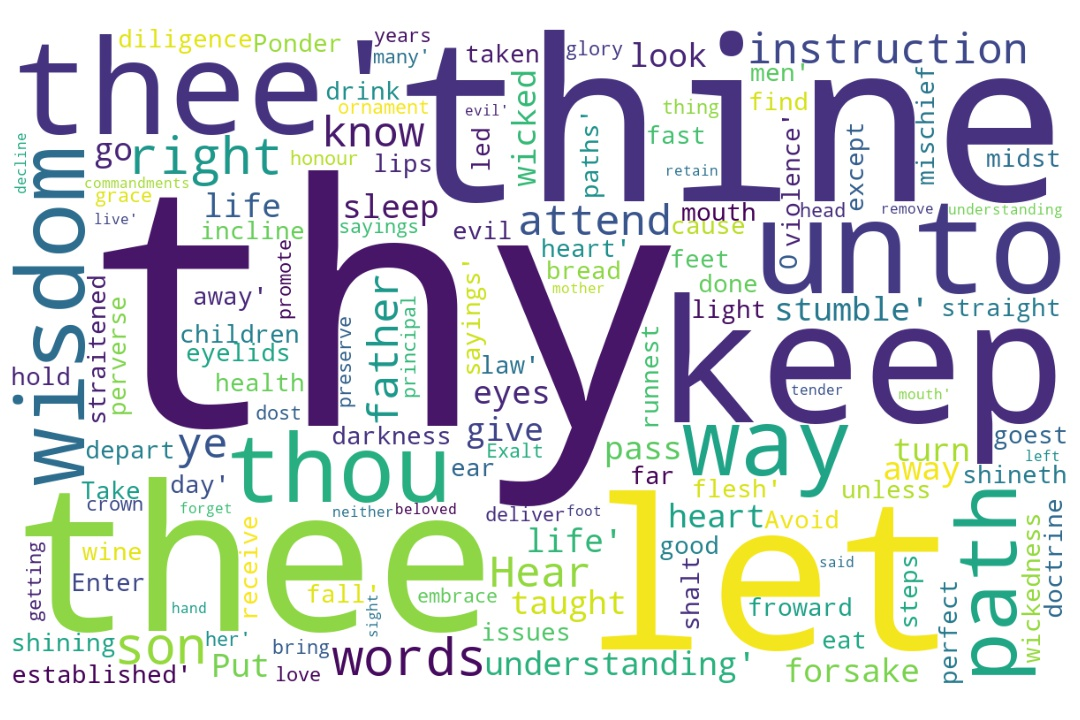
\includegraphics[width=\linewidth]{20OT-Proverbs/Proverb4-WordCloud.jpg}
  \caption{Proverb 4 Word Cloud}
  \label{fig:Proverb 4 Word Cloud}
\end{figure}

% [cmyk]{0.99998,1,0,0}{
%\marginpar{\scriptsize \textcolor[rgb]{0.00,0.545,0.269}{$\rightarrow$7 Princes:  (1) Carshena, (2) Shethar, (3) Admatha, (4) Tarshish, (5) Meres, %(6) Marsena, and (7) Memucan.}}
\marginpar{\scriptsize \centering \fcolorbox{bone}{lime}{\textbf{WHAT WISDOM DOES}}\\ (Proverb 4:1--27) 
\begin{compactenum}[I.][8]
    \item \textbf{Contains Instructions that Liberate} \index[scripture]{Proverbs!Pro 04:13} (Pro 4:13)
    \item \textbf{Corrects Ill-Conceived Lies} \index[scripture]{Proverbs!Pro 04:14-19} (Pro 4:14-19)
    \item \textbf{Counteracts Ill-focused Living} \index[scripture]{Proverbs!Pro 04:14-19} (Pro 4:14-19) 
    \item \textbf{Contains Illuminating Light} \index[scripture]{Proverbs!Pro 04:18}(Pro 4:18) 
    \item \textbf{Condemns the Ignorant Losers} \index[scripture]{Proverbs!Pro 04:19}(Pro 4:19)
    \item \textbf{Covers the Issues of Life} \index[scripture]{Proverbs!Pro 04:22}(Pro 4:22)
    \item \textbf{Challenges Us to Incessant Learning} \index[scripture]{Proverbs!Pro 04:23}(Pro 4:23) 
\end{compactenum} }

\marginpar{\scriptsize \centering \fcolorbox{bone}{yellow}{\textbf{INSTRUCTIONS CONCERNING}}\\
 \fcolorbox{bone}{yellow}{\textbf{WISDOM}} \\ (Proverb 4:1--27) 

\textbf{Introduction}: Scripture has much to say concerning wisdom.
\begin{compactenum}[I.][8]
\item \textbf{Regard It} \index[scripture]{Proverbs!Pro 04:01}(Pro 4:1)
\item \textbf{Retain It} \index[scripture]{Proverbs!Pro 04:04}(Pro 4:4)
\item \textbf{Reach for It} \index[scripture]{Proverbs!Pro 04:05}(Pro 4:5)
\item \textbf{Remember it as a Priority} \index[scripture]{Proverbs!Pro 04:05}(Pro 4:5)
\item \textbf{Reject what is Not Wisdom} \index[scripture]{Proverbs!Pro 04:14--15}(Pro 4:14-15)
\item \textbf{Realise what Wisdom Provides} \index[scripture]{Proverbs!Pro 04:21--22}(Pro 4:21-22)
\item \textbf{Reflect upon the Wisdom of your Ways} \index[scripture]{Proverbs!Pro 04:26}(Pro 4:26)
\end{compactenum} }

\marginpar{\scriptsize \centering \fcolorbox{bone}{black}{\textbf{\textcolor[cmyk]{0,0,0,0}{DESIRING WISDOM}}}\\ (Proverb 4:1--27) 
\begin{compactenum}[I.][8]
    \item \textbf{Realize its Practical Benefits} \index[scripture]{Proverbs!Pro 04:01-27}(Pro 4:1-27)
    \item \textbf{Make it a Priority} \index[scripture]{Proverbs!Pro 04:07} (Pro 4:7)
    \item \textbf{Recognize the Principles of Wisdom} \index[scripture]{Proverbs!Pro 04:01}(Pro 4:1)
    \item \textbf{Expect it to Promote You} \index[scripture]{Proverbs!Pro 04:08, 09}(Pro 4:8, 9) 
    \item \textbf{Expect it to Preserve You} \index[scripture]{Proverbs!Pro 04:22}(Pro 4:22) 
    \item \textbf{Should Be a Preoccupation} \index[scripture]{Proverbs!Pro 04:20-22}(Pro 4:20-22) 
    \item \textbf{Revel in its Presence}  \index[scripture]{Proverbs!Pro 04:08}(Pro 4:8) 
    \item \textbf{Regard it as Precious} \index[scripture]{Proverbs!Pro 04:13}(Pro 4:13) 
\end{compactenum} }

\marginpar{\scriptsize \centering\fcolorbox{black}{blue}{\textbf{\textcolor[cmyk]{0,0,0,0}{KNOWLEDGE, WISDOM}}}\\\fcolorbox{black}{blue}{\textbf{\textcolor[cmyk]{0,0,0,0}{\& UNDERSTANDING}}}\\  \fcolorbox{black}{blue}{\textbf{\textcolor[cmyk]{0,0,0,0}{IN CONTEXT}}}\\ (Proverb 4:1-27) 
\begin{compactenum}[I.][7]
    \item A \textbf{Father's Care} (Pro 4:1)
    \item A \textbf{Faithful Choice} (Pro 4:1-27)
    \item A \textbf{Firm Consideration} (Pro 4:1-27)
    \item A \textbf{First Concern} (Pro 4:7)
    \item A \textbf{Final Crown} (Pro 4:9)
    \item A \textbf{Full Course} (Pro 4:10)
    \item A \textbf{Future Challenge} (Pro 4:5, 6, 7, 8, 13)
\end{compactenum} }

% arginpar{\scriptsize \centering \fcolorbox{bone}{lime}{\textbf{INSTRUCTION CONCERNING WSDOM}}\\ 
% \marginpar{\scriptsize \centering \fcolorbox{bone}{yellow}{\textbf{INSTRUCTIONd CONCERNING WSDOM}}\\ 
% \marginpar{\scriptsize \centering \fcolorbox{bone}{black}{\textbf{\textcolor[cmyk]{0,0,0,0}{DESIRING WISDOM}}}\\ 
% \marginpar{\scriptsize \centering \fcolorbox{black}{blue}{\textbf{\textcolor[cmyk]{0,0,0,0}{GOING TOWARD UNDERSTANDING}}}\\ (Passage) 
% \marginpar{\scriptsize \centering \fcolorbox{black}{ForestGreen}{\textbf{\textcolor[cmyk]{0,0,0,0}{EXAMPLE}}}\\ (Proverbs 4:1-27) 


\footnote{\textcolor[cmyk]{0.99998,1,0,0}{\hyperlink{TOC}{Return to end of Table of Contents.}}}\footnote{\href{https://audiobible.com/bible/bible.html}{\textcolor[cmyk]{0.99998,1,0,0}{Proverbs Audio}}}\textcolor[cmyk]{0.99998,1,0,0}{Hear, ye children, the instruction of a father, and attend to know understanding.}\footnote{\textbf{Proverb 1:8} - My son, hear the instruction of thy father, and forsake not the law of thy mother:}\footnote{\textbf{Proverb 5:1} - My son, attend unto my wisdom, and bow thine ear to my understanding:}\footnote{\textbf{Proverb 8:32-36} - Now therefore hearken unto me, O ye children: for blessed are they that keep my ways. Hear instruction, and be wise, and refuse it not. Blessed is the man that heareth me, watching daily at my gates, waiting at the posts of my doors. For whoso findeth me findeth life, and shall obtain favour of the LORD. But he that sinneth against me wrongeth his own soul: all they that hate me love death.}\footnote{\textbf{Hebrews 2:1} - Therefore we ought to give the more earnest heed to the things which we have heard, lest at any time we should let them slip.}
[2] \textcolor[cmyk]{0.99998,1,0,0}{For I give you good doctrine, forsake ye \fcolorbox{bone}{bone}{not} my law.}
[3] \textcolor[cmyk]{0.99998,1,0,0}{For I was my father's son, tender and only \emph{beloved} in the sight of my mother.}
[4] \textcolor[cmyk]{0.99998,1,0,0}{He taught me also, and said unto me, Let thine heart retain my words: keep my commandments, and live.}
[5] \textcolor[cmyk]{0.99998,1,0,0}{Get wisdom, get understanding: forget \emph{it} \fcolorbox{bone}{bone}{not}; neither decline from the words of my mouth.}
[6] \textcolor[cmyk]{0.99998,1,0,0}{Forsake her \fcolorbox{bone}{bone}{not}, and she shall preserve thee: love her, and she shall keep thee.}
[7] \textcolor[cmyk]{0.99998,1,0,0}{Wisdom \emph{is} the principal thing; \emph{therefore} get wisdom: and with all thy getting get understanding.}
[8] \textcolor[cmyk]{0.99998,1,0,0}{Exalt her, and she shall promote thee: she shall bring thee to honour, when thou dost embrace her.}
[9] \textcolor[cmyk]{0.99998,1,0,0}{She shall give to thine head an ornament of grace: a crown of glory shall she deliver to thee.}
[10] \textcolor[cmyk]{0.99998,1,0,0}{Hear, O my son, and receive my sayings; and the years of thy life shall be many.}
[11] \textcolor[cmyk]{0.99998,1,0,0}{I have taught thee in the way of wisdom; I have led thee in right paths.}
[12] \textcolor[cmyk]{0.99998,1,0,0}{When thou goest, thy steps shall \fcolorbox{bone}{bone}{not} be straitened; and when thou runnest, thou shalt \fcolorbox{bone}{bone}{not} stumble.}
[13] \textcolor[cmyk]{0.99998,1,0,0}{Take fast hold of instruction; let \emph{her} \fcolorbox{bone}{bone}{not} go: keep her; for \fcolorbox{bone}{lime}{she \emph{is} thy life}.}\\
\\
\P \textcolor[cmyk]{0.99998,1,0,0}{\fcolorbox{bone}{lime}{Enter \fcolorbox{bone}{bone}{not}} into the path of the wicked, and go \fcolorbox{bone}{bone}{not} in the way of evil \emph{men}.}
[15] \textcolor[cmyk]{0.99998,1,0,0}{Avoid it, pass \fcolorbox{bone}{bone}{not} by it, \fcolorbox{bone}{lime}{turn from it}, and pass away.}
[16] \textcolor[cmyk]{0.99998,1,0,0}{For they sleep \fcolorbox{bone}{bone}{not}, except they have done mischief; and their sleep is taken away, unless they cause \emph{some} to fall.}
[17] \textcolor[cmyk]{0.99998,1,0,0}{For they eat the bread of wickedness, and drink the wine of violence.}
[18] \textcolor[cmyk]{0.99998,1,0,0}{But the path of the just \emph{is} as the \fcolorbox{bone}{lime}{shining light}, that shineth more and more unto the perfect day.}
[19] \textcolor[cmyk]{0.99998,1,0,0}{The way of the wicked \emph{is} as \fcolorbox{bone}{lime}{darkness}: they know \fcolorbox{bone}{bone}{not} at what they stumble.}\\
\\
\P \textcolor[cmyk]{0.99998,1,0,0}{My son, attend to my words; incline thine ear unto my sayings.}
[21] \textcolor[cmyk]{0.99998,1,0,0}{Let them \fcolorbox{bone}{bone}{not} depart from thine eyes; keep them in the midst of thine heart.}
[22] \textcolor[cmyk]{0.99998,1,0,0}{For \fcolorbox{bone}{lime}{they \emph{are} life} unto those that find them, and health to all their flesh.}\\
\\
\P \textcolor[cmyk]{0.99998,1,0,0}{Keep thy heart with all \fcolorbox{bone}{lime}{diligence}; for out of it \emph{are} the issues of life.}
[24] \textcolor[cmyk]{0.99998,1,0,0}{Put away from thee a froward mouth, and perverse lips put far from thee.}
[25] \textcolor[cmyk]{0.99998,1,0,0}{Let thine eyes look right on, and let thine eyelids look straight before thee.} 
[26] \textcolor[cmyk]{0.99998,1,0,0}{Ponder the path of thy feet, and let all thy ways be established.}
[27] \textcolor[cmyk]{0.99998,1,0,0}{Turn \fcolorbox{bone}{bone}{not} to the right hand nor to the left: remove thy foot from evil.}

\marginpar{\scriptsize \centering \fcolorbox{bone}{orange}{\textbf{GOING TOWARD}}
\fcolorbox{bone}{orange}{\textbf{UNDERSTANDING}}\\ (Proverb 4:1-27) 

\begin{compactenum}[I.][7]
    \item \textbf{Preservation}  \index[scripture]{Proverbs!Pro 04:06} (Pro 4:6)
    \item The \textbf{Principal} Thing \index[scripture]{Proverbs!Pro 04:07} (Pro 4:7)
    \item \textbf{Promotion}  \index[scripture]{Proverbs!Pro 04:08} (Pro 4:8)
    \item \textbf{Paths}  \index[scripture]{Proverbs!Pro 04:14} (Pro 4:14)
    \item A \textbf{Perfect} Day \index[scripture]{Proverbs!Pro 04:18} (Pro 4:18)
    \item  \textbf{Preversity}  \index[scripture]{Proverbs!Pro 04:24} (Pro 4:24)
    \item  \textbf{Ponderings}  \index[scripture]{Proverbs!Pro 04:26} (Pro 4:26)
\end{compactenum} }


\index[NWIV]{13!Proverbs!Pro 4:1}\index[AWIP]{Hear!Proverbs!Pro 4:1}\index[AWIP]{ye!Proverbs!Pro 4:1}\index[AWIP]{children!Proverbs!Pro 4:1}\index[AWIP]{the!Proverbs!Pro 4:1}\index[AWIP]{instruction!Proverbs!Pro 4:1}\index[AWIP]{of!Proverbs!Pro 4:1}\index[AWIP]{a!Proverbs!Pro 4:1}\index[AWIP]{father!Proverbs!Pro 4:1}\index[AWIP]{and!Proverbs!Pro 4:1}\index[AWIP]{attend!Proverbs!Pro 4:1}\index[AWIP]{to!Proverbs!Pro 4:1}\index[AWIP]{know!Proverbs!Pro 4:1}\index[AWIP]{understanding!Proverbs!Pro 4:1}

\index[NWIV]{11!Proverbs!Pro 4:2}\index[AWIP]{For!Proverbs!Pro 4:2}\index[AWIP]{I!Proverbs!Pro 4:2}\index[AWIP]{give!Proverbs!Pro 4:2}\index[AWIP]{you!Proverbs!Pro 4:2}\index[AWIP]{good!Proverbs!Pro 4:2}\index[AWIP]{doctrine!Proverbs!Pro 4:2}\index[AWIP]{forsake!Proverbs!Pro 4:2}\index[AWIP]{ye!Proverbs!Pro 4:2}\index[AWIP]{not!Proverbs!Pro 4:2}\index[AWIP]{my!Proverbs!Pro 4:2}\index[AWIP]{law!Proverbs!Pro 4:2}

\index[NWIV]{16!Proverbs!Pro 4:3}\index[AWIP]{For!Proverbs!Pro 4:3}\index[AWIP]{I!Proverbs!Pro 4:3}\index[AWIP]{was!Proverbs!Pro 4:3}\index[AWIP]{my!Proverbs!Pro 4:3}\index[AWIP]{my!Proverbs!Pro 4:3 (2)}\index[AWIP]{father's!Proverbs!Pro 4:3}\index[AWIP]{son!Proverbs!Pro 4:3}\index[AWIP]{tender!Proverbs!Pro 4:3}\index[AWIP]{and!Proverbs!Pro 4:3}\index[AWIP]{only!Proverbs!Pro 4:3}\index[AWIP]{\emph{beloved}!Proverbs!Pro 4:3}\index[AWIP]{in!Proverbs!Pro 4:3}\index[AWIP]{the!Proverbs!Pro 4:3}\index[AWIP]{sight!Proverbs!Pro 4:3}\index[AWIP]{of!Proverbs!Pro 4:3}\index[AWIP]{mother!Proverbs!Pro 4:3}\index[AWIP]{\emph{beloved}!Proverbs!Pro 4:3}

\index[NWIV]{19!Proverbs!Pro 4:4}\index[AWIP]{He!Proverbs!Pro 4:4}\index[AWIP]{taught!Proverbs!Pro 4:4}\index[AWIP]{me!Proverbs!Pro 4:4}\index[AWIP]{me!Proverbs!Pro 4:4 (2)}\index[AWIP]{also!Proverbs!Pro 4:4}\index[AWIP]{and!Proverbs!Pro 4:4}\index[AWIP]{and!Proverbs!Pro 4:4 (2)}\index[AWIP]{said!Proverbs!Pro 4:4}\index[AWIP]{unto!Proverbs!Pro 4:4}\index[AWIP]{Let!Proverbs!Pro 4:4}\index[AWIP]{thine!Proverbs!Pro 4:4}\index[AWIP]{heart!Proverbs!Pro 4:4}\index[AWIP]{retain!Proverbs!Pro 4:4}\index[AWIP]{my!Proverbs!Pro 4:4}\index[AWIP]{my!Proverbs!Pro 4:4 (2)}\index[AWIP]{words!Proverbs!Pro 4:4}\index[AWIP]{keep!Proverbs!Pro 4:4}\index[AWIP]{commandments!Proverbs!Pro 4:4}\index[AWIP]{live!Proverbs!Pro 4:4}

\index[NWIV]{15!Proverbs!Pro 4:5}\index[AWIP]{Get!Proverbs!Pro 4:5}\index[AWIP]{wisdom!Proverbs!Pro 4:5}\index[AWIP]{get!Proverbs!Pro 4:5}\index[AWIP]{understanding!Proverbs!Pro 4:5}\index[AWIP]{forget!Proverbs!Pro 4:5}\index[AWIP]{\emph{it}!Proverbs!Pro 4:5}\index[AWIP]{not!Proverbs!Pro 4:5}\index[AWIP]{neither!Proverbs!Pro 4:5}\index[AWIP]{decline!Proverbs!Pro 4:5}\index[AWIP]{from!Proverbs!Pro 4:5}\index[AWIP]{the!Proverbs!Pro 4:5}\index[AWIP]{words!Proverbs!Pro 4:5}\index[AWIP]{of!Proverbs!Pro 4:5}\index[AWIP]{my!Proverbs!Pro 4:5}\index[AWIP]{mouth!Proverbs!Pro 4:5}\index[AWIP]{\emph{it}!Proverbs!Pro 4:5}

\index[NWIV]{15!Proverbs!Pro 4:6}\index[AWIP]{Forsake!Proverbs!Pro 4:6}\index[AWIP]{her!Proverbs!Pro 4:6}\index[AWIP]{her!Proverbs!Pro 4:6 (2)}\index[AWIP]{not!Proverbs!Pro 4:6}\index[AWIP]{and!Proverbs!Pro 4:6}\index[AWIP]{and!Proverbs!Pro 4:6 (2)}\index[AWIP]{she!Proverbs!Pro 4:6}\index[AWIP]{she!Proverbs!Pro 4:6 (2)}\index[AWIP]{shall!Proverbs!Pro 4:6}\index[AWIP]{shall!Proverbs!Pro 4:6 (2)}\index[AWIP]{preserve!Proverbs!Pro 4:6}\index[AWIP]{thee!Proverbs!Pro 4:6}\index[AWIP]{thee!Proverbs!Pro 4:6 (2)}\index[AWIP]{love!Proverbs!Pro 4:6}\index[AWIP]{keep!Proverbs!Pro 4:6}

\index[NWIV]{15!Proverbs!Pro 4:7}\index[AWIP]{Wisdom!Proverbs!Pro 4:7}\index[AWIP]{\emph{is}!Proverbs!Pro 4:7}\index[AWIP]{the!Proverbs!Pro 4:7}\index[AWIP]{principal!Proverbs!Pro 4:7}\index[AWIP]{thing!Proverbs!Pro 4:7}\index[AWIP]{\emph{therefore}!Proverbs!Pro 4:7}\index[AWIP]{get!Proverbs!Pro 4:7}\index[AWIP]{get!Proverbs!Pro 4:7 (2)}\index[AWIP]{wisdom!Proverbs!Pro 4:7}\index[AWIP]{and!Proverbs!Pro 4:7}\index[AWIP]{with!Proverbs!Pro 4:7}\index[AWIP]{all!Proverbs!Pro 4:7}\index[AWIP]{thy!Proverbs!Pro 4:7}\index[AWIP]{getting!Proverbs!Pro 4:7}\index[AWIP]{understanding!Proverbs!Pro 4:7}\index[AWIP]{\emph{is}!Proverbs!Pro 4:7}\index[AWIP]{\emph{therefore}!Proverbs!Pro 4:7}

\index[NWIV]{18!Proverbs!Pro 4:8}\index[AWIP]{Exalt!Proverbs!Pro 4:8}\index[AWIP]{her!Proverbs!Pro 4:8}\index[AWIP]{her!Proverbs!Pro 4:8 (2)}\index[AWIP]{and!Proverbs!Pro 4:8}\index[AWIP]{she!Proverbs!Pro 4:8}\index[AWIP]{she!Proverbs!Pro 4:8 (2)}\index[AWIP]{shall!Proverbs!Pro 4:8}\index[AWIP]{shall!Proverbs!Pro 4:8 (2)}\index[AWIP]{promote!Proverbs!Pro 4:8}\index[AWIP]{thee!Proverbs!Pro 4:8}\index[AWIP]{thee!Proverbs!Pro 4:8 (2)}\index[AWIP]{bring!Proverbs!Pro 4:8}\index[AWIP]{to!Proverbs!Pro 4:8}\index[AWIP]{honour!Proverbs!Pro 4:8}\index[AWIP]{when!Proverbs!Pro 4:8}\index[AWIP]{thou!Proverbs!Pro 4:8}\index[AWIP]{dost!Proverbs!Pro 4:8}\index[AWIP]{embrace!Proverbs!Pro 4:8}

\index[NWIV]{19!Proverbs!Pro 4:9}\index[AWIP]{She!Proverbs!Pro 4:9}\index[AWIP]{shall!Proverbs!Pro 4:9}\index[AWIP]{shall!Proverbs!Pro 4:9 (2)}\index[AWIP]{give!Proverbs!Pro 4:9}\index[AWIP]{to!Proverbs!Pro 4:9}\index[AWIP]{to!Proverbs!Pro 4:9 (2)}\index[AWIP]{thine!Proverbs!Pro 4:9}\index[AWIP]{head!Proverbs!Pro 4:9}\index[AWIP]{an!Proverbs!Pro 4:9}\index[AWIP]{ornament!Proverbs!Pro 4:9}\index[AWIP]{of!Proverbs!Pro 4:9}\index[AWIP]{of!Proverbs!Pro 4:9 (2)}\index[AWIP]{grace!Proverbs!Pro 4:9}\index[AWIP]{a!Proverbs!Pro 4:9}\index[AWIP]{crown!Proverbs!Pro 4:9}\index[AWIP]{glory!Proverbs!Pro 4:9}\index[AWIP]{she!Proverbs!Pro 4:9}\index[AWIP]{deliver!Proverbs!Pro 4:9}\index[AWIP]{thee!Proverbs!Pro 4:9}

\index[NWIV]{17!Proverbs!Pro 4:10}\index[AWIP]{Hear!Proverbs!Pro 4:10}\index[AWIP]{O!Proverbs!Pro 4:10}\index[AWIP]{my!Proverbs!Pro 4:10}\index[AWIP]{my!Proverbs!Pro 4:10 (2)}\index[AWIP]{son!Proverbs!Pro 4:10}\index[AWIP]{and!Proverbs!Pro 4:10}\index[AWIP]{and!Proverbs!Pro 4:10 (2)}\index[AWIP]{receive!Proverbs!Pro 4:10}\index[AWIP]{sayings!Proverbs!Pro 4:10}\index[AWIP]{the!Proverbs!Pro 4:10}\index[AWIP]{years!Proverbs!Pro 4:10}\index[AWIP]{of!Proverbs!Pro 4:10}\index[AWIP]{thy!Proverbs!Pro 4:10}\index[AWIP]{life!Proverbs!Pro 4:10}\index[AWIP]{shall!Proverbs!Pro 4:10}\index[AWIP]{be!Proverbs!Pro 4:10}\index[AWIP]{many!Proverbs!Pro 4:10}

\index[NWIV]{16!Proverbs!Pro 4:11}\index[AWIP]{I!Proverbs!Pro 4:11}\index[AWIP]{I!Proverbs!Pro 4:11 (2)}\index[AWIP]{have!Proverbs!Pro 4:11}\index[AWIP]{have!Proverbs!Pro 4:11 (2)}\index[AWIP]{taught!Proverbs!Pro 4:11}\index[AWIP]{thee!Proverbs!Pro 4:11}\index[AWIP]{thee!Proverbs!Pro 4:11 (2)}\index[AWIP]{in!Proverbs!Pro 4:11}\index[AWIP]{in!Proverbs!Pro 4:11 (2)}\index[AWIP]{the!Proverbs!Pro 4:11}\index[AWIP]{way!Proverbs!Pro 4:11}\index[AWIP]{of!Proverbs!Pro 4:11}\index[AWIP]{wisdom!Proverbs!Pro 4:11}\index[AWIP]{led!Proverbs!Pro 4:11}\index[AWIP]{right!Proverbs!Pro 4:11}\index[AWIP]{paths!Proverbs!Pro 4:11}

\index[NWIV]{17!Proverbs!Pro 4:12}\index[AWIP]{When!Proverbs!Pro 4:12}\index[AWIP]{thou!Proverbs!Pro 4:12}\index[AWIP]{thou!Proverbs!Pro 4:12 (2)}\index[AWIP]{thou!Proverbs!Pro 4:12 (3)}\index[AWIP]{goest!Proverbs!Pro 4:12}\index[AWIP]{thy!Proverbs!Pro 4:12}\index[AWIP]{steps!Proverbs!Pro 4:12}\index[AWIP]{shall!Proverbs!Pro 4:12}\index[AWIP]{not!Proverbs!Pro 4:12}\index[AWIP]{not!Proverbs!Pro 4:12 (2)}\index[AWIP]{be!Proverbs!Pro 4:12}\index[AWIP]{straitened!Proverbs!Pro 4:12}\index[AWIP]{and!Proverbs!Pro 4:12}\index[AWIP]{when!Proverbs!Pro 4:12}\index[AWIP]{runnest!Proverbs!Pro 4:12}\index[AWIP]{shalt!Proverbs!Pro 4:12}\index[AWIP]{stumble!Proverbs!Pro 4:12}

\index[NWIV]{16!Proverbs!Pro 4:13}\index[AWIP]{Take!Proverbs!Pro 4:13}\index[AWIP]{fast!Proverbs!Pro 4:13}\index[AWIP]{hold!Proverbs!Pro 4:13}\index[AWIP]{of!Proverbs!Pro 4:13}\index[AWIP]{instruction!Proverbs!Pro 4:13}\index[AWIP]{let!Proverbs!Pro 4:13}\index[AWIP]{\emph{her}!Proverbs!Pro 4:13}\index[AWIP]{not!Proverbs!Pro 4:13}\index[AWIP]{go!Proverbs!Pro 4:13}\index[AWIP]{keep!Proverbs!Pro 4:13}\index[AWIP]{her!Proverbs!Pro 4:13}\index[AWIP]{for!Proverbs!Pro 4:13}\index[AWIP]{she!Proverbs!Pro 4:13}\index[AWIP]{\emph{is}!Proverbs!Pro 4:13}\index[AWIP]{thy!Proverbs!Pro 4:13}\index[AWIP]{life!Proverbs!Pro 4:13}\index[AWIP]{\emph{her}!Proverbs!Pro 4:13}\index[AWIP]{\emph{is}!Proverbs!Pro 4:13}

\index[NWIV]{17!Proverbs!Pro 4:14}\index[AWIP]{Enter!Proverbs!Pro 4:14}\index[AWIP]{not!Proverbs!Pro 4:14}\index[AWIP]{not!Proverbs!Pro 4:14 (2)}\index[AWIP]{into!Proverbs!Pro 4:14}\index[AWIP]{the!Proverbs!Pro 4:14}\index[AWIP]{the!Proverbs!Pro 4:14 (2)}\index[AWIP]{the!Proverbs!Pro 4:14 (3)}\index[AWIP]{path!Proverbs!Pro 4:14}\index[AWIP]{of!Proverbs!Pro 4:14}\index[AWIP]{of!Proverbs!Pro 4:14 (2)}\index[AWIP]{wicked!Proverbs!Pro 4:14}\index[AWIP]{and!Proverbs!Pro 4:14}\index[AWIP]{go!Proverbs!Pro 4:14}\index[AWIP]{in!Proverbs!Pro 4:14}\index[AWIP]{way!Proverbs!Pro 4:14}\index[AWIP]{evil!Proverbs!Pro 4:14}\index[AWIP]{\emph{men}!Proverbs!Pro 4:14}\index[AWIP]{\emph{men}!Proverbs!Pro 4:14}

\index[NWIV]{12!Proverbs!Pro 4:15}\index[AWIP]{Avoid!Proverbs!Pro 4:15}\index[AWIP]{it!Proverbs!Pro 4:15}\index[AWIP]{it!Proverbs!Pro 4:15 (2)}\index[AWIP]{it!Proverbs!Pro 4:15 (3)}\index[AWIP]{pass!Proverbs!Pro 4:15}\index[AWIP]{pass!Proverbs!Pro 4:15 (2)}\index[AWIP]{not!Proverbs!Pro 4:15}\index[AWIP]{by!Proverbs!Pro 4:15}\index[AWIP]{turn!Proverbs!Pro 4:15}\index[AWIP]{from!Proverbs!Pro 4:15}\index[AWIP]{and!Proverbs!Pro 4:15}\index[AWIP]{away!Proverbs!Pro 4:15}

\index[NWIV]{21!Proverbs!Pro 4:16}\index[AWIP]{For!Proverbs!Pro 4:16}\index[AWIP]{they!Proverbs!Pro 4:16}\index[AWIP]{they!Proverbs!Pro 4:16 (2)}\index[AWIP]{they!Proverbs!Pro 4:16 (3)}\index[AWIP]{sleep!Proverbs!Pro 4:16}\index[AWIP]{sleep!Proverbs!Pro 4:16 (2)}\index[AWIP]{not!Proverbs!Pro 4:16}\index[AWIP]{except!Proverbs!Pro 4:16}\index[AWIP]{have!Proverbs!Pro 4:16}\index[AWIP]{done!Proverbs!Pro 4:16}\index[AWIP]{mischief!Proverbs!Pro 4:16}\index[AWIP]{and!Proverbs!Pro 4:16}\index[AWIP]{their!Proverbs!Pro 4:16}\index[AWIP]{is!Proverbs!Pro 4:16}\index[AWIP]{taken!Proverbs!Pro 4:16}\index[AWIP]{away!Proverbs!Pro 4:16}\index[AWIP]{unless!Proverbs!Pro 4:16}\index[AWIP]{cause!Proverbs!Pro 4:16}\index[AWIP]{\emph{some}!Proverbs!Pro 4:16}\index[AWIP]{to!Proverbs!Pro 4:16}\index[AWIP]{fall!Proverbs!Pro 4:16}\index[AWIP]{\emph{some}!Proverbs!Pro 4:16}

\index[NWIV]{13!Proverbs!Pro 4:17}\index[AWIP]{For!Proverbs!Pro 4:17}\index[AWIP]{they!Proverbs!Pro 4:17}\index[AWIP]{eat!Proverbs!Pro 4:17}\index[AWIP]{the!Proverbs!Pro 4:17}\index[AWIP]{the!Proverbs!Pro 4:17 (2)}\index[AWIP]{bread!Proverbs!Pro 4:17}\index[AWIP]{of!Proverbs!Pro 4:17}\index[AWIP]{of!Proverbs!Pro 4:17 (2)}\index[AWIP]{wickedness!Proverbs!Pro 4:17}\index[AWIP]{and!Proverbs!Pro 4:17}\index[AWIP]{drink!Proverbs!Pro 4:17}\index[AWIP]{wine!Proverbs!Pro 4:17}\index[AWIP]{violence!Proverbs!Pro 4:17}

\index[NWIV]{20!Proverbs!Pro 4:18}\index[AWIP]{But!Proverbs!Pro 4:18}\index[AWIP]{the!Proverbs!Pro 4:18}\index[AWIP]{the!Proverbs!Pro 4:18 (2)}\index[AWIP]{the!Proverbs!Pro 4:18 (3)}\index[AWIP]{the!Proverbs!Pro 4:18 (4)}\index[AWIP]{path!Proverbs!Pro 4:18}\index[AWIP]{of!Proverbs!Pro 4:18}\index[AWIP]{just!Proverbs!Pro 4:18}\index[AWIP]{\emph{is}!Proverbs!Pro 4:18}\index[AWIP]{as!Proverbs!Pro 4:18}\index[AWIP]{shining!Proverbs!Pro 4:18}\index[AWIP]{light!Proverbs!Pro 4:18}\index[AWIP]{that!Proverbs!Pro 4:18}\index[AWIP]{shineth!Proverbs!Pro 4:18}\index[AWIP]{more!Proverbs!Pro 4:18}\index[AWIP]{more!Proverbs!Pro 4:18 (2)}\index[AWIP]{and!Proverbs!Pro 4:18}\index[AWIP]{unto!Proverbs!Pro 4:18}\index[AWIP]{perfect!Proverbs!Pro 4:18}\index[AWIP]{day!Proverbs!Pro 4:18}\index[AWIP]{\emph{is}!Proverbs!Pro 4:18}

\index[NWIV]{15!Proverbs!Pro 4:19}\index[AWIP]{The!Proverbs!Pro 4:19}\index[AWIP]{way!Proverbs!Pro 4:19}\index[AWIP]{of!Proverbs!Pro 4:19}\index[AWIP]{the!Proverbs!Pro 4:19}\index[AWIP]{wicked!Proverbs!Pro 4:19}\index[AWIP]{\emph{is}!Proverbs!Pro 4:19}\index[AWIP]{as!Proverbs!Pro 4:19}\index[AWIP]{darkness!Proverbs!Pro 4:19}\index[AWIP]{they!Proverbs!Pro 4:19}\index[AWIP]{they!Proverbs!Pro 4:19 (2)}\index[AWIP]{know!Proverbs!Pro 4:19}\index[AWIP]{not!Proverbs!Pro 4:19}\index[AWIP]{at!Proverbs!Pro 4:19}\index[AWIP]{what!Proverbs!Pro 4:19}\index[AWIP]{stumble!Proverbs!Pro 4:19}\index[AWIP]{\emph{is}!Proverbs!Pro 4:19}

\index[NWIV]{12!Proverbs!Pro 4:20}\index[AWIP]{My!Proverbs!Pro 4:20}\index[AWIP]{son!Proverbs!Pro 4:20}\index[AWIP]{attend!Proverbs!Pro 4:20}\index[AWIP]{to!Proverbs!Pro 4:20}\index[AWIP]{my!Proverbs!Pro 4:20}\index[AWIP]{my!Proverbs!Pro 4:20 (2)}\index[AWIP]{words!Proverbs!Pro 4:20}\index[AWIP]{incline!Proverbs!Pro 4:20}\index[AWIP]{thine!Proverbs!Pro 4:20}\index[AWIP]{ear!Proverbs!Pro 4:20}\index[AWIP]{unto!Proverbs!Pro 4:20}\index[AWIP]{sayings!Proverbs!Pro 4:20}

\index[NWIV]{15!Proverbs!Pro 4:21}\index[AWIP]{Let!Proverbs!Pro 4:21}\index[AWIP]{them!Proverbs!Pro 4:21}\index[AWIP]{them!Proverbs!Pro 4:21 (2)}\index[AWIP]{not!Proverbs!Pro 4:21}\index[AWIP]{depart!Proverbs!Pro 4:21}\index[AWIP]{from!Proverbs!Pro 4:21}\index[AWIP]{thine!Proverbs!Pro 4:21}\index[AWIP]{thine!Proverbs!Pro 4:21 (2)}\index[AWIP]{eyes!Proverbs!Pro 4:21}\index[AWIP]{keep!Proverbs!Pro 4:21}\index[AWIP]{in!Proverbs!Pro 4:21}\index[AWIP]{the!Proverbs!Pro 4:21}\index[AWIP]{midst!Proverbs!Pro 4:21}\index[AWIP]{of!Proverbs!Pro 4:21}\index[AWIP]{heart!Proverbs!Pro 4:21}

\index[NWIV]{15!Proverbs!Pro 4:22}\index[AWIP]{For!Proverbs!Pro 4:22}\index[AWIP]{they!Proverbs!Pro 4:22}\index[AWIP]{\emph{are}!Proverbs!Pro 4:22}\index[AWIP]{life!Proverbs!Pro 4:22}\index[AWIP]{unto!Proverbs!Pro 4:22}\index[AWIP]{those!Proverbs!Pro 4:22}\index[AWIP]{that!Proverbs!Pro 4:22}\index[AWIP]{find!Proverbs!Pro 4:22}\index[AWIP]{them!Proverbs!Pro 4:22}\index[AWIP]{and!Proverbs!Pro 4:22}\index[AWIP]{health!Proverbs!Pro 4:22}\index[AWIP]{to!Proverbs!Pro 4:22}\index[AWIP]{all!Proverbs!Pro 4:22}\index[AWIP]{their!Proverbs!Pro 4:22}\index[AWIP]{flesh!Proverbs!Pro 4:22}\index[AWIP]{\emph{are}!Proverbs!Pro 4:22}

\index[NWIV]{15!Proverbs!Pro 4:23}\index[AWIP]{Keep!Proverbs!Pro 4:23}\index[AWIP]{thy!Proverbs!Pro 4:23}\index[AWIP]{heart!Proverbs!Pro 4:23}\index[AWIP]{with!Proverbs!Pro 4:23}\index[AWIP]{all!Proverbs!Pro 4:23}\index[AWIP]{diligence!Proverbs!Pro 4:23}\index[AWIP]{for!Proverbs!Pro 4:23}\index[AWIP]{out!Proverbs!Pro 4:23}\index[AWIP]{of!Proverbs!Pro 4:23}\index[AWIP]{of!Proverbs!Pro 4:23 (2)}\index[AWIP]{it!Proverbs!Pro 4:23}\index[AWIP]{\emph{are}!Proverbs!Pro 4:23}\index[AWIP]{the!Proverbs!Pro 4:23}\index[AWIP]{issues!Proverbs!Pro 4:23}\index[AWIP]{life!Proverbs!Pro 4:23}\index[AWIP]{\emph{are}!Proverbs!Pro 4:23}

\index[NWIV]{14!Proverbs!Pro 4:24}\index[AWIP]{Put!Proverbs!Pro 4:24}\index[AWIP]{away!Proverbs!Pro 4:24}\index[AWIP]{from!Proverbs!Pro 4:24}\index[AWIP]{from!Proverbs!Pro 4:24 (2)}\index[AWIP]{thee!Proverbs!Pro 4:24}\index[AWIP]{thee!Proverbs!Pro 4:24 (2)}\index[AWIP]{a!Proverbs!Pro 4:24}\index[AWIP]{froward!Proverbs!Pro 4:24}\index[AWIP]{mouth!Proverbs!Pro 4:24}\index[AWIP]{and!Proverbs!Pro 4:24}\index[AWIP]{perverse!Proverbs!Pro 4:24}\index[AWIP]{lips!Proverbs!Pro 4:24}\index[AWIP]{put!Proverbs!Pro 4:24}\index[AWIP]{far!Proverbs!Pro 4:24}

\index[NWIV]{14!Proverbs!Pro 4:25}\index[AWIP]{Let!Proverbs!Pro 4:25}\index[AWIP]{thine!Proverbs!Pro 4:25}\index[AWIP]{thine!Proverbs!Pro 4:25 (2)}\index[AWIP]{eyes!Proverbs!Pro 4:25}\index[AWIP]{look!Proverbs!Pro 4:25}\index[AWIP]{look!Proverbs!Pro 4:25 (2)}\index[AWIP]{right!Proverbs!Pro 4:25}\index[AWIP]{on!Proverbs!Pro 4:25}\index[AWIP]{and!Proverbs!Pro 4:25}\index[AWIP]{let!Proverbs!Pro 4:25}\index[AWIP]{eyelids!Proverbs!Pro 4:25}\index[AWIP]{straight!Proverbs!Pro 4:25}\index[AWIP]{before!Proverbs!Pro 4:25}\index[AWIP]{thee!Proverbs!Pro 4:25}

\index[NWIV]{13!Proverbs!Pro 4:26}\index[AWIP]{Ponder!Proverbs!Pro 4:26}\index[AWIP]{the!Proverbs!Pro 4:26}\index[AWIP]{path!Proverbs!Pro 4:26}\index[AWIP]{of!Proverbs!Pro 4:26}\index[AWIP]{thy!Proverbs!Pro 4:26}\index[AWIP]{thy!Proverbs!Pro 4:26 (2)}\index[AWIP]{feet!Proverbs!Pro 4:26}\index[AWIP]{and!Proverbs!Pro 4:26}\index[AWIP]{let!Proverbs!Pro 4:26}\index[AWIP]{all!Proverbs!Pro 4:26}\index[AWIP]{ways!Proverbs!Pro 4:26}\index[AWIP]{be!Proverbs!Pro 4:26}\index[AWIP]{established!Proverbs!Pro 4:26}

\index[NWIV]{15!Proverbs!Pro 4:27}\index[AWIP]{Turn!Proverbs!Pro 4:27}\index[AWIP]{not!Proverbs!Pro 4:27}\index[AWIP]{to!Proverbs!Pro 4:27}\index[AWIP]{to!Proverbs!Pro 4:27 (2)}\index[AWIP]{the!Proverbs!Pro 4:27}\index[AWIP]{the!Proverbs!Pro 4:27 (2)}\index[AWIP]{right!Proverbs!Pro 4:27}\index[AWIP]{hand!Proverbs!Pro 4:27}\index[AWIP]{nor!Proverbs!Pro 4:27}\index[AWIP]{left!Proverbs!Pro 4:27}\index[AWIP]{remove!Proverbs!Pro 4:27}\index[AWIP]{thy!Proverbs!Pro 4:27}\index[AWIP]{foot!Proverbs!Pro 4:27}\index[AWIP]{from!Proverbs!Pro 4:27}\index[AWIP]{evil!Proverbs!Pro 4:27}


\section{Proverb 4 Outlines}

\subsection{My Outlines}

\subsubsection{What Wisdom Does!}
It:
\index[speaker]{Keith Anthony!Proverb 04 (What Wisdom Does)}
\index[series]{Proverbs (Keith Anthony)!Pro 04 (What Wisdom Does)}
\index[date]{2014/11/03!Proverb 04 (What Wisdom Does) (Keith Anthony)}
\begin{compactenum}[I.][8]
    \item \textbf{Contains Instructions that Liberate} \index[scripture]{Proverbs!Pro 04:13} (Pro 4:13)
    \item \textbf{Corrects Ill-Conceived Lies} \index[scripture]{Proverbs!Pro 04:14-19} (Pro 4:14-19)
    \item \textbf{Counteracts Ill-focused Living} \index[scripture]{Proverbs!Pro 04:14-19} (Pro 4:14-19) 
    \item \textbf{Contains Illuminating Light} \index[scripture]{Proverbs!Pro 04:18}(Pro 4:18) 
    \item \textbf{Condemns the Ignorant Losers} \index[scripture]{Proverbs!Pro 04:19}(Pro 4:19)
    \item \textbf{Covers the Issues of Life} \index[scripture]{Proverbs!Pro 04:22}(Pro 4:22)
    \item \textbf{Challenges Us to Incessant Learning} \index[scripture]{Proverbs!Pro 04:23}(Pro 4:23) 
\end{compactenum}


\subsubsection{Instructions Concerning Wisdom}
\index[speaker]{Keith Anthony!Proverb 04 (Instructions Concerning Wisdom)}
\index[series]{Proverbs (Keith Anthony)!Pro 04 (Instructions Concerning Wisdom)}
\index[date]{2016/05/03!Proverb 04 (Instructions Concerning Wisdom) (Keith Anthony)}
%\textbf{Lineage}: adpated from S. Conway\\
\textbf{Introduction}: Scripture has much to say concerning wisdom.
\begin{compactenum}[I.][8]
\item \textbf{Regard It} \index[scripture]{Proverbs!Pro 04:01}(Pro 4:1)
\item \textbf{Retain It} \index[scripture]{Proverbs!Pro 04:04}(Pro 4:4)
\item \textbf{Reach for It} \index[scripture]{Proverbs!Pro 04:05}(Pro 4:5)
\item \textbf{Remember it as a Priority} \index[scripture]{Proverbs!Pro 04:05}(Pro 4:5)
\item \textbf{Reject what is Not Wisdom} \index[scripture]{Proverbs!Pro 04:14--15}(Pro 4:14-15)
\item \textbf{Realise what Wisdom Provides} \index[scripture]{Proverbs!Pro 04:21--22}(Pro 4:21-22)
\item \textbf{Reflect upon the Wisdom of your Ways} \index[scripture]{Proverbs!Pro 04:26}(Pro 4:26)
\end{compactenum}

\subsubsection{Desiring Wisdom}
What should our attitude be concerning wisdom?
\index[speaker]{Keith Anthony!Proverb 04 (Desiring Wisdom)}
\index[series]{Proverbs (Keith Anthony)!Pro 04 (Desiring Wisdom)}
\index[date]{2014/11/03!Proverb 04 (Desiring Wisdom) (Keith Anthony)}
\begin{compactenum}[I.][8]
    \item \textbf{Realize its Practical Benefits} \index[scripture]{Proverbs!Pro 04:01-27}(Pro 4:1-27)
    \item \textbf{Make it a Priority} \index[scripture]{Proverbs!Pro 04:07} (Pro 4:7)
    \item \textbf{Recognize the Principles of Wisdom} \index[scripture]{Proverbs!Pro 04:01}(Pro 4:1)
    \item \textbf{Expect it to Promote You} \index[scripture]{Proverbs!Pro 04:08, 09}(Pro 4:8, 9) 
    \item \textbf{Expect it to Preserve You} \index[scripture]{Proverbs!Pro 04:22}(Pro 4:22) 
    \item \textbf{Should Be a Preoccupation} \index[scripture]{Proverbs!Pro 04:20-22}(Pro 4:20-22) 
    \item \textbf{Revel in its Presence}  \index[scripture]{Proverbs!Pro 04:08}(Pro 4:8) 
    \item \textbf{Regard it as Precious} \index[scripture]{Proverbs!Pro 04:13}(Pro 4:13) 
\end{compactenum}

\subsubsection{Knowledge, Understanding \& Wisdom, in Context}
\textbf{Introduction: }Thinking about wisdom and life, and perspective, where should it be in a young man's list of priorities?
\index[speaker]{Keith Anthony!Proverb 04 (Knowledge, Understanding \& Wisdom, in Context)}
\index[series]{Proverbs (Keith Anthony)!Pro 04 (Knowledge, Understanding \& Wisdom, in Context)}
\index[date]{2015/07/04!Proverb 04 (Knowledge, Understanding \& Wisdom, in Context) (Keith Anthony)}
\begin{compactenum}[I.][7]
    \item A \textbf{Father's Care} (Pro 4:1)
    \item A \textbf{Faithful Choice} (Pro 4:1-27)
    \item A \textbf{Firm Consideration} (Pro 4:1-27)
    \item A \textbf{First Concern} (Pro 4:7)
    \item A \textbf{Final Crown} (Pro 4:9)
    \item A \textbf{Full Course} (Pro 4:10)
    \item A \textbf{Future Challenge} (Pro 4:5, 6, 7, 8, 13)
\end{compactenum}

\subsubsection{Going Toward Understanding}
%\textbf{Introduction: }Thinking about wisdom and life, and perspective, where should it be in a young man's list of priorities?
\index[speaker]{Keith Anthony!Proverb 04 (Going Toward Understanding)}
\index[series]{Proverbs (Keith Anthony)!Pro 04 (Going Toward Understanding)}
\index[date]{2018/06/04!Proverb 04 (Going Toward Understanding) (Keith Anthony)}
\begin{compactenum}[I.][7]
    \item \textbf{Preservation}  \index[scripture]{Proverbs!Pro 04:06} (Pro 4:6)
    \item The \textbf{Principal} Thing \index[scripture]{Proverbs!Pro 04:07} (Pro 4:7)
    \item \textbf{Promotion}  \index[scripture]{Proverbs!Pro 04:08} (Pro 4:8)
    \item \textbf{Paths}  \index[scripture]{Proverbs!Pro 04:14} (Pro 4:14)
    \item A \textbf{Perfect} Day \index[scripture]{Proverbs!Pro 04:18} (Pro 4:18)
    \item  \textbf{Preversity}  \index[scripture]{Proverbs!Pro 04:24} (Pro 4:24)
    \item  \textbf{Ponderings}  \index[scripture]{Proverbs!Pro 04:26} (Pro 4:26)
\end{compactenum}
\subsection{Outlines from Acar}


\subsubsection{Self-Discipline}
\index[speaker]{Epafras T. Acar!Proverb 04:23-27 (Self-Discipline)}
\index[series]{Proverbs (Epafras T. Acar)!Prov 04:23-27 (Self-Discipline)}
\index[date]{2018/09/14!Proverb 04:23-27 (Self-Discipline) Epafras T. Acar)}
%\textbf{Lineage}: adpated from S. Conway\\
\textbf{Introduction}: How to be self-disciplined?  By being careful with...\\
\\
\begin{compactenum}[I.][4]
	\item THE WORDS OF YOUR MOUTH, Proverbs 4:24 
	\begin{compactenum}[A.]
		\item Bad Words- “Put away from thee a froward mouth...”
		\item Belligerent Words -“...and perverse lips put far from thee.”
	\end{compactenum}
	\item THE WANTS OF YOUR EYES, Proverbs 4:25 
	\begin{compactenum}[A.]
		\item Focus on Your Goal - “Let thine eyes look right on...”
		\item Fix your Gaze -“...and let thine eyelids look straight before thee.”
	\end{compactenum}
	\item THE WAYS OF YOUR FEET, Proverbs 4:26, 27
	\begin{compactenum}[A.]
		\item Meditate on Your Ways - “Ponder the path of thy feet...”
		\item Manage Your Ways  - “...and let all thy ways be established.”
		\begin{compactenum}[1.]
			\item You Straighten your Way- “Turn not to the right hand nor to the left...”
			\item You Separate from Evil  - “...remove thy foot from evil.”
		\end{compactenum}
	\end{compactenum}
\end{compactenum}

\textbf{Conclusion}:  Therefore be careful with the words that you speak, the things that you watch, and the ways that you walk on. The fruit of all these attitudes and actions is a self-disciplined life.

\index[FACEBOOK]{SIMPLE SERMON OUTLINES \& QUOTES!Epafras T. Acar (Self-Discipline) - Proverb 04:23-27!2016/01/20}


%\subsubsection{Guard Your Heart}
%\textbf{Introduction: }Fairweather Mountain is one of the most spectacular mountains North America. Located off the southeast coast of Alaska, the mountain reaches 15,000 feet above sea level. Massive granite walls with deep ravines cut by cascading glaciers create an inspiring view. This view, however, can only be seen about twenty days a year when the weather is fair. The mountain is called Fairweather because you can only see the full glory and beauty of the mountain when the fog clears.
%Author, John Eldredge, uses Fairweather Mountain as an illustration to describe how most people live their lives.  Much of our confusion results from a failure to understand the truth proclaimed in Proverbs 4:23 and other Scriptures that describe the significance of the heart. In this brief passage, the wise king Solomon identified four principles of guarding our heart.\footnote{online: \href{https://www.lifeway.com/en/articles/sermon-guard-your-heart-part-1-proverbs-4}{Guard Your Heart}}
%\index[speaker]{Steve Andrews!Proverbs 04:23 (Guard Your Heart)}
%\index[series]{Proverbs (Steve Andrews)!Proverbs 04:23 (Guard Your Heart)}
%\index[date]{2014/01/01!Proverbs 04:23 (Guard Your Heart) (Steve Andrews)}
%\index{event}{Graduation (Scott A Thomas)!Proverbs 04 (Get Wisdom)}
%\begin{compactenum}[I.][4]
%    \item \textbf{Wisdom's Significance}
%    \begin{compactenum}[A.]
%        \item Wisdom is the Principal Thing (Proverbs 4:4-7)
%        \item Wisdom is the Powerful Thing (Proverbs 4:8-10)
%        \begin{compactenum}[1.]
%            \item The Promotion comes when you Exalt Wisdom.
%            \item The Prestige comes when you Embrace Wisdom.
%            \item The Prize comes when you Enjoy Wisdom.
 %       \end{compactenum}
%    \end{compactenum}
%    \item \textbf{Wisdom's Sources}
%    \begin{compactenum}[A.]
%        \item Wisdom Comes from the Great God (James 1:5)
%        \begin{compactenum}[1.]
%            \item Your Steps will not be Straightened (Proverbs 4:12)
 %           \item Your Shoes will not be Stumbling (Proverbs 4;12b)
%            \item Your Sheens will not be Suffering
%            \begin{compactenum}[1.]
%                \item No Hindrances on this road called grace.
%                \item No Holes will on this road called grace.
%            \end{compactenum}
%        \end{compactenum}
%        \item Wisdom Comes from the Godly Guardians (Proverbs 12:1)
%        \begin{compactenum}[1.]
%            \item We do well to Listen to Godly Parental Wisdom.
%            \item We do well to Look to Godly Parental Wisdom.
%        \end{compactenum}
%    \end{compactenum}
%    \item \textbf{Wisdom Strays}
%    \begin{compactenum}[A.]
%        \item If we run off with Worldliness, Wisdom will run off in the opposite direction\!
%        \begin{compactenum}[1.]
%            \item Without Wisdom Life gets Sideways.
%            \item Without Wisdom Life gets Stupid.
%        \end{compactenum}
%        \item If we run off with Wickedness, Wisdom will run off in the opposite direction.
%        \begin{compactenum}[1.]
%            \item Wander off in Wickedness and Wisdom leaves.
%            \item Waller on into Wickedness and Wisdom leaves.
%        \end{compactenum}
%    \end{compactenum}
%    \item \textbf{Wisdom Sticks} (Proverbs 12:13)
%    \begin{compactenum}[A.]
%        \item Make Wisdom Your Life  (Proverbs 12:4, 9)
%        \begin{compactenum}[1.]
%            \item It will give you a Charm of Grace
%            \item It will give you a Crown of Glory
%        \end{compactenum}
%        \item Make Wisdom Your Love (Proverbs 12:6)
%        \begin{compactenum}[1.]
%            \item Learn to Love the Book of Wisdom\!
%            \item Learn to Love the Beauty of Wisdom\!
%        \end{compactenum}
%    \end{compactenum}
%\end{compactenum}
%\textbf{Conclusion: }
%\begin{compactenum}[1.]
%    \item We all need wisdom\!
%    \begin{compactenum}[a.]
%        \item Wisdom about our Decisions.
%        \item Wisdom about our Directions.
%        \item Wisdom about our Destiny.
%    \end{compactenum}
%    \item Perhaps you would like to come and ask God for wisdom about your decisions, your directions, and your destiny.
%    \item Perhaps you’re a parent and you need to come and pray for wisdom for yourself and for your children.
%\end{compactenum}



\subsection{Outlines from Eades}


\subsubsection{Brighter the Pathway Grows}
\index[speaker]{Brian Eades!Proverb 04:18 (Brighter the Pathway Grows)}
\index[series]{Proverbs (Brian Eades)!Pro 04:18 (Brighter the Pathway Grows)}
\index[date]{2018/09/14!Proverb 04:18 (Brighter the Pathway Grows) (Brian Eades)}
%\textbf{Lineage}: adpated from S. Conway\\
\textbf{Introduction}: The bright pathway is the pathway of the just. The path of darkness is only reserved for those who are lost and have rejected Christ.
\begin{compactenum}[I.][4]
	\item The \textbf{Inspired Path} \footnote{Brian Eades, Sermon Hints}
	\item The \textbf{Imputed Path}
	\item The \textbf{Illuminated Path}
	\item The \textbf{Invincible Path}
	\item The \textbf{Infinite Path}
	\item The \textbf{Imputed Path}
	\item The \textbf{Icreasing Path}
\end{compactenum}

\index[FACEBOOK]{SERMON HINTS!Brian Eades (Brighter the Pathway Grows) - Proverb 04:18!2016/01/20}


%\subsubsection{Guard Your Heart}
%\textbf{Introduction: }Fairweather Mountain is one of the most spectacular mountains North America. Located off the southeast coast of Alaska, the mountain reaches 15,000 feet above sea level. Massive granite walls with deep ravines cut by cascading glaciers create an inspiring view. This view, however, can only be seen about twenty days a year when the weather is fair. The mountain is called Fairweather because you can only see the full glory and beauty of the mountain when the fog clears.
%Author, John Eldredge, uses Fairweather Mountain as an illustration to describe how most people live their lives.  Much of our confusion results from a failure to understand the truth proclaimed in Proverbs 4:23 and other Scriptures that describe the significance of the heart. In this brief passage, the wise king Solomon identified four principles of guarding our heart.\footnote{online: \href{https://www.lifeway.com/en/articles/sermon-guard-your-heart-part-1-proverbs-4}{Guard Your Heart}}
%\index[speaker]{Steve Andrews!Proverbs 04:23 (Guard Your Heart)}
%\index[series]{Proverbs (Steve Andrews)!Proverbs 04:23 (Guard Your Heart)}
%\index[date]{2014/01/01!Proverbs 04:23 (Guard Your Heart) (Steve Andrews)}
%\index{event}{Graduation (Scott A Thomas)!Proverbs 04 (Get Wisdom)}
%\begin{compactenum}[I.][4]
%    \item \textbf{Wisdom's Significance}
%    \begin{compactenum}[A.]
%        \item Wisdom is the Principal Thing (Proverbs 4:4-7)
%        \item Wisdom is the Powerful Thing (Proverbs 4:8-10)
%        \begin{compactenum}[1.]
%            \item The Promotion comes when you Exalt Wisdom.
%            \item The Prestige comes when you Embrace Wisdom.
%            \item The Prize comes when you Enjoy Wisdom.
 %       \end{compactenum}
%    \end{compactenum}
%    \item \textbf{Wisdom's Sources}
%    \begin{compactenum}[A.]
%        \item Wisdom Comes from the Great God (James 1:5)
%        \begin{compactenum}[1.]
%            \item Your Steps will not be Straightened (Proverbs 4:12)
 %           \item Your Shoes will not be Stumbling (Proverbs 4;12b)
%            \item Your Sheens will not be Suffering
%            \begin{compactenum}[1.]
%                \item No Hindrances on this road called grace.
%                \item No Holes will on this road called grace.
%            \end{compactenum}
%        \end{compactenum}
%        \item Wisdom Comes from the Godly Guardians (Proverbs 12:1)
%        \begin{compactenum}[1.]
%            \item We do well to Listen to Godly Parental Wisdom.
%            \item We do well to Look to Godly Parental Wisdom.
%        \end{compactenum}
%    \end{compactenum}
%    \item \textbf{Wisdom Strays}
%    \begin{compactenum}[A.]
%        \item If we run off with Worldliness, Wisdom will run off in the opposite direction\!
%        \begin{compactenum}[1.]
%            \item Without Wisdom Life gets Sideways.
%            \item Without Wisdom Life gets Stupid.
%        \end{compactenum}
%        \item If we run off with Wickedness, Wisdom will run off in the opposite direction.
%        \begin{compactenum}[1.]
%            \item Wander off in Wickedness and Wisdom leaves.
%            \item Waller on into Wickedness and Wisdom leaves.
%        \end{compactenum}
%    \end{compactenum}
%    \item \textbf{Wisdom Sticks} (Proverbs 12:13)
%    \begin{compactenum}[A.]
%        \item Make Wisdom Your Life  (Proverbs 12:4, 9)
%        \begin{compactenum}[1.]
%            \item It will give you a Charm of Grace
%            \item It will give you a Crown of Glory
%        \end{compactenum}
%        \item Make Wisdom Your Love (Proverbs 12:6)
%        \begin{compactenum}[1.]
%            \item Learn to Love the Book of Wisdom\!
%            \item Learn to Love the Beauty of Wisdom\!
%        \end{compactenum}
%    \end{compactenum}
%\end{compactenum}
%\textbf{Conclusion: }
%\begin{compactenum}[1.]
%    \item We all need wisdom\!
%    \begin{compactenum}[a.]
%        \item Wisdom about our Decisions.
%        \item Wisdom about our Directions.
%        \item Wisdom about our Destiny.
%    \end{compactenum}
%    \item Perhaps you would like to come and ask God for wisdom about your decisions, your directions, and your destiny.
%    \item Perhaps you’re a parent and you need to come and pray for wisdom for yourself and for your children.
%\end{compactenum}



\subsection{Outlines from Jalla}


\subsubsection{Keep thy heart with all Diligence}
\index[speaker]{Alvin Jalla!Proverb 04:23 (Keep thy heart with all diligence)}
\index[series]{Proverbs (Alvin Jalla)!Prov 04:23 (Keep thy heart with all diligence)}
\index[date]{2020/05/29!Proverb 04:23 (Keep thy heart with all diligence) Alvin Jalla)}
%\textbf{Lineage}: adpated from S. Conway\\
\textbf{Introduction}: Keep thy heart with all diligence; for out of it are issues of life.
A Heart for God that build a Godly Relationship\\
\\
\begin{compactenum}[I.][4]
	\item A submissive heart 
	\item A servant heart
	\item A surrendered heart
\end{compactenum}

\textbf{Conclusion}:  Therefore be careful with the words that you speak, the things that you watch, and the ways that you walk on. The fruit of all these attitudes and actions is a self-disciplined life.

\index[FACEBOOK]{SIMPLE SERMON OUTLINES \& QUOTES!Alvin Jalla (Keep thy heart with all Diligence) - Proverb 04:23!2020/05/29}


%\subsubsection{Guard Your Heart}
%\textbf{Introduction: }Fairweather Mountain is one of the most spectacular mountains North America. Located off the southeast coast of Alaska, the mountain reaches 15,000 feet above sea level. Massive granite walls with deep ravines cut by cascading glaciers create an inspiring view. This view, however, can only be seen about twenty days a year when the weather is fair. The mountain is called Fairweather because you can only see the full glory and beauty of the mountain when the fog clears.
%Author, John Eldredge, uses Fairweather Mountain as an illustration to describe how most people live their lives.  Much of our confusion results from a failure to understand the truth proclaimed in Proverbs 4:23 and other Scriptures that describe the significance of the heart. In this brief passage, the wise king Solomon identified four principles of guarding our heart.\footnote{online: \href{https://www.lifeway.com/en/articles/sermon-guard-your-heart-part-1-proverbs-4}{Guard Your Heart}}
%\index[speaker]{Steve Andrews!Proverbs 04:23 (Guard Your Heart)}
%\index[series]{Proverbs (Steve Andrews)!Proverbs 04:23 (Guard Your Heart)}
%\index[date]{2014/01/01!Proverbs 04:23 (Guard Your Heart) (Steve Andrews)}
%\index{event}{Graduation (Scott A Thomas)!Proverbs 04 (Get Wisdom)}
%\begin{compactenum}[I.][4]
%    \item \textbf{Wisdom's Significance}
%    \begin{compactenum}[A.]
%        \item Wisdom is the Principal Thing (Proverbs 4:4-7)
%        \item Wisdom is the Powerful Thing (Proverbs 4:8-10)
%        \begin{compactenum}[1.]
%            \item The Promotion comes when you Exalt Wisdom.
%            \item The Prestige comes when you Embrace Wisdom.
%            \item The Prize comes when you Enjoy Wisdom.
 %       \end{compactenum}
%    \end{compactenum}
%    \item \textbf{Wisdom's Sources}
%    \begin{compactenum}[A.]
%        \item Wisdom Comes from the Great God (James 1:5)
%        \begin{compactenum}[1.]
%            \item Your Steps will not be Straightened (Proverbs 4:12)
 %           \item Your Shoes will not be Stumbling (Proverbs 4;12b)
%            \item Your Sheens will not be Suffering
%            \begin{compactenum}[1.]
%                \item No Hindrances on this road called grace.
%                \item No Holes will on this road called grace.
%            \end{compactenum}
%        \end{compactenum}
%        \item Wisdom Comes from the Godly Guardians (Proverbs 12:1)
%        \begin{compactenum}[1.]
%            \item We do well to Listen to Godly Parental Wisdom.
%            \item We do well to Look to Godly Parental Wisdom.
%        \end{compactenum}
%    \end{compactenum}
%    \item \textbf{Wisdom Strays}
%    \begin{compactenum}[A.]
%        \item If we run off with Worldliness, Wisdom will run off in the opposite direction\!
%        \begin{compactenum}[1.]
%            \item Without Wisdom Life gets Sideways.
%            \item Without Wisdom Life gets Stupid.
%        \end{compactenum}
%        \item If we run off with Wickedness, Wisdom will run off in the opposite direction.
%        \begin{compactenum}[1.]
%            \item Wander off in Wickedness and Wisdom leaves.
%            \item Waller on into Wickedness and Wisdom leaves.
%        \end{compactenum}
%    \end{compactenum}
%    \item \textbf{Wisdom Sticks} (Proverbs 12:13)
%    \begin{compactenum}[A.]
%        \item Make Wisdom Your Life  (Proverbs 12:4, 9)
%        \begin{compactenum}[1.]
%            \item It will give you a Charm of Grace
%            \item It will give you a Crown of Glory
%        \end{compactenum}
%        \item Make Wisdom Your Love (Proverbs 12:6)
%        \begin{compactenum}[1.]
%            \item Learn to Love the Book of Wisdom\!
%            \item Learn to Love the Beauty of Wisdom\!
%        \end{compactenum}
%    \end{compactenum}
%\end{compactenum}
%\textbf{Conclusion: }
%\begin{compactenum}[1.]
%    \item We all need wisdom\!
%    \begin{compactenum}[a.]
%        \item Wisdom about our Decisions.
%        \item Wisdom about our Directions.
%        \item Wisdom about our Destiny.
%    \end{compactenum}
%    \item Perhaps you would like to come and ask God for wisdom about your decisions, your directions, and your destiny.
%    \item Perhaps you’re a parent and you need to come and pray for wisdom for yourself and for your children.
%\end{compactenum}



\subsection{Outlines from Thomas}

\subsubsection{Get Wisdom}
\textbf{Introduction: }Schools are known for testing and testing and then testing the test and then testing the teacher who gave the test. After all that, they will finally give you a certificate or diploma that states that you took the test and have been educated to a certain level. We’ve all been there, but that does not mean that you and I have got all the wisdom. Let me challenge all of us concerning Wisdom.\footnote{10 June 2016, Scott A Thomas}
\index[speaker]{Scott A Thomas!Proverb 04:46 (Get Wisdom)}
\index[series]{Proverbs (Scott A Thomas) Pro 04:46 (Get Wisdom)}
\index[date]{2016/06/09!Proverb 04:46 (Get Wisdom) (Scott A Thomas)}

%\index{event}{Graduation (Scott A Thomas)!Proverbs 04 (Get Wisdom)}

\begin{compactenum}[I.][4]
    \item \textbf{Wisdom's Significance}
    \begin{compactenum}[A.]
        \item Wisdom is the Principal Thing (Pro 4:4-7)
        \item Wisdom is the Powerful Thing (Pro 4:8-10)
        \begin{compactenum}[1.]
            \item The Promotion comes when you Exalt Wisdom.
            \item The Prestige comes when you Embrace Wisdom.
            \item The Prize comes when you Enjoy Wisdom.
        \end{compactenum}
    \end{compactenum}
    \item \textbf{Wisdom's Sources}
    \begin{compactenum}[A.]
        \item Wisdom Comes from the Great God (James 1:5)
        \begin{compactenum}[1.]
            \item Your Steps will not be Straightened (Pro 4:12)
            \item Your Shoes will not be Stumbling (Pro 4;12b)
            \item Your Sheens will not be Suffering
            \begin{compactenum}[1.]
                \item No Hindrances on this road called grace.
                \item No Holes will on this road called grace.
            \end{compactenum}
        \end{compactenum}
        \item Wisdom Comes from the Godly Guardians (Pro 12:1)
        \begin{compactenum}[1.]
            \item We do well to Listen to Godly Parental Wisdom.
            \item We do well to Look to Godly Parental Wisdom.
        \end{compactenum}
    \end{compactenum}
    \item \textbf{Wisdom Strays}
    \begin{compactenum}[A.]
        \item If we run off with Worldliness, Wisdom will run off in the opposite direction\!
        \begin{compactenum}[1.]
            \item Without Wisdom Life gets Sideways.
            \item Without Wisdom Life gets Stupid.
        \end{compactenum}
        \item If we run off with Wickedness, Wisdom will run off in the opposite direction.
        \begin{compactenum}[1.]
            \item Wander off in Wickedness and Wisdom leaves.
            \item Waller on into Wickedness and Wisdom leaves.
        \end{compactenum}
    \end{compactenum}
    \item \textbf{Wisdom Sticks} (Pro 12:13)
    \begin{compactenum}[A.]
        \item Make Wisdom Your Life  (Pro 12:4, 9)
        \begin{compactenum}[1.]
            \item It will give you a Charm of Grace
            \item It will give you a Crown of Glory
        \end{compactenum}
        \item Make Wisdom Your Love (Proverbs 12:6)
        \begin{compactenum}[1.]
            \item Learn to Love the Book of Wisdom\!
            \item Learn to Love the Beauty of Wisdom\!
        \end{compactenum}
    \end{compactenum}
\end{compactenum}
\textbf{Conclusion: }
\begin{compactenum}[1.]
    \item We all need wisdom\!
    \begin{compactenum}[a.]
        \item Wisdom about our Decisions.
        \item Wisdom about our Directions.
        \item Wisdom about our Destiny.
    \end{compactenum}
    \item Perhaps you would like to come and ask God for wisdom about your decisions, your directions, and your destiny.
    \item Perhaps you’re a parent and you need to come and pray for wisdom for yourself and for your children.
\end{compactenum}

\index[FACEBOOK]{FUNDAMENTAL BAPTIST SERMON OUTLINES!Scott Thomas - Proverb 04!2016/06/09}


\subsubsection{Ponder the Path}
\textbf{Introduction: }Schools are known for testing and testing and then testing the test and then testing the teacher who gave the test. After all that, they will finally give you a certificate or diploma that states that you took the test and have been educated to a certain level. We’ve all been there, but that does not mean that you and I have got all the wisdom. Let me challenge all of us concerning Wisdom.\footnote{10 June 2016, Scott A Thomas}
\index[speaker]{Scott A Thomas!Proverb 04 (Ponder the Path)}
\index[series]{Proverbs (Scott A Thomas)!Pro 04 (Ponder the Path)}
\index[date]{2016/06/09!Proverb 04 (Ponder the Path) (Scott A Thomas)}

\textbf{Introduction: }
\begin{compactenum}
	\item Notice the \textbf{Education and Ponder the Path}
**This is a father instructing his son in wisdom telling him and showing him the difference between right paths and wrong paths. 
Proverbs 4:11  11 I have taught thee in the way of wisdom; I have led thee in right paths.
Proverbs 4:14  14 Enter not into the path of the wicked, and go not in the way of evil men.
Proverbs 4:18  18 But the path of the just is as the shining light, that shineth more and more unto the perfect day.
**Then in Proverbs 4:26, he says, “Son – Ponder the Path and get established!”
**Oh how I wish those friends, loved ones, and past church people would just ponder the path and look back for a moment.  
**Has your path been a walk with the Savior and the Holy Spirit, or with sin and Satan?
**We must take a look and ponder the path!
	\item Notice the \textbf{Embracing  and Ponder the Path}
	\item Notice the \textbf{Enjoyment   and Ponder the Path}
\end{compactenum}


\begin{compactenum}[I.][4]
    \item \textbf{Wisdom's Significance}
    \begin{compactenum}[A.]
        \item Wisdom is the Principal Thing (Pro 4:4-7)
        \item Wisdom is the Powerful Thing (Pro 4:8-10)
        \begin{compactenum}[1.]
            \item The Promotion comes when you Exalt Wisdom.
            \item The Prestige comes when you Embrace Wisdom.
            \item The Prize comes when you Enjoy Wisdom.
        \end{compactenum}
    \end{compactenum}
    \item \textbf{Wisdom's Sources}
    \begin{compactenum}[A.]
        \item Wisdom Comes from the Great God (James 1:5)
        \begin{compactenum}[1.]
            \item Your Steps will not be Straightened (Pro 4:12)
            \item Your Shoes will not be Stumbling (Pro 4;12b)
            \item Your Sheens will not be Suffering
            \begin{compactenum}[1.]
                \item No Hindrances on this road called grace.
                \item No Holes will on this road called grace.
            \end{compactenum}
        \end{compactenum}
        \item Wisdom Comes from the Godly Guardians (Pro 12:1)
        \begin{compactenum}[1.]
            \item We do well to Listen to Godly Parental Wisdom.
            \item We do well to Look to Godly Parental Wisdom.
        \end{compactenum}
    \end{compactenum}
    \item \textbf{Wisdom Strays}
    \begin{compactenum}[A.]
        \item If we run off with Worldliness, Wisdom will run off in the opposite direction\!
        \begin{compactenum}[1.]
            \item Without Wisdom Life gets Sideways.
            \item Without Wisdom Life gets Stupid.
        \end{compactenum}
        \item If we run off with Wickedness, Wisdom will run off in the opposite direction.
        \begin{compactenum}[1.]
            \item Wander off in Wickedness and Wisdom leaves.
            \item Waller on into Wickedness and Wisdom leaves.
        \end{compactenum}
    \end{compactenum}
    \item \textbf{Wisdom Sticks} (Pro 12:13)
    \begin{compactenum}[A.]
        \item Make Wisdom Your Life  (Pro 12:4, 9)
        \begin{compactenum}[1.]
            \item It will give you a Charm of Grace
            \item It will give you a Crown of Glory
        \end{compactenum}
        \item Make Wisdom Your Love (Proverbs 12:6)
        \begin{compactenum}[1.]
            \item Learn to Love the Book of Wisdom\!
            \item Learn to Love the Beauty of Wisdom\!
        \end{compactenum}
    \end{compactenum}
\end{compactenum}
\textbf{Conclusion: }
\begin{compactenum}[1.]
    \item We all need wisdom\!
    \begin{compactenum}[a.]
        \item Wisdom about our Decisions.
        \item Wisdom about our Directions.
        \item Wisdom about our Destiny.
    \end{compactenum}
    \item Perhaps you would like to come and ask God for wisdom about your decisions, your directions, and your destiny.
    \item Perhaps you’re a parent and you need to come and pray for wisdom for yourself and for your children.
\end{compactenum}

\index[FACEBOOK]{FUNDAMENTAL BAPTIST SERMON OUTLINES!Scott Thomas - Proverb 04:46!2018/09/23}


%%% For Indexes

%\index[DEVOTIONAL]{TGIF1!Os Hillman (Living for a Cause Greater Than Yourself) - Proverb 19:17!2021/12/21}

%\index[DEVOTIONAL]{TGIF1!Os Hillman (Living for a Cause Greater Than Yourself) - Proverb 19:17!2021/12/21}

















%%% colour: cardinal red - \textcolor[cmyk]{0,0.85,0.70,0.23}{text}


%%%% Example marginpar with a compactenum list --- green color text
%\marginpar{\scriptsize \textcolor[rgb]{0.00,0.545,0.269}{$\rightarrow$7 Abominations: 
%\begin{compactenum}
%	\item A proud look,
%	\item a lying tongue,
%	\item hands that shed innocent blood,
%	\item An heart that deviseth wicked imaginations,
%	\item feet that be swift in running to mischief,
%	\item A false witness that speaketh lies, and
%	\item he that soweth discord among brethren.
%\end{compactenum}}}



%\newpage

%\begin{mdframed}[style=MyFrame]
%\begin{center}
%\begin{longtable}{|p{.5in}|p{3.5in}|}

%\caption[Corruption Alert: Proverbs 18:1]{Corruption Alert: Proverbs 18:1} \label{table:CorruptionProv18:1} \\ 

%\hline  
%\multicolumn{1}{|c|}{\textbf{Version}} & 
%\multicolumn{1}{c|}{\textbf{Corruption}}  \\ \hline 
%\endfirsthead
 
%\multicolumn{2}{c}
%{{\bfseries \tablename\ \thetable{} -- continued from previous page}} \\  \hline  
%\multicolumn{1}{|c|}{\textbf{Version}} & 
%\multicolumn{1}{c|}{\textbf{Corruption}}  \\ \hline 
%\endhead
 
%\hline \multicolumn{2}{|r|}{{Continued on next page}} \\ \hline
%\endfoot 
%\textcolor[rgb]{0.00,0.00,1.00}{AV} & \textcolor[rgb]{0.00,0.00,1.00}{Through desire a man, having separated himself, seeketh \emph{and} intermeddleth with all wisdom.} \\ \hline
%
%ASV &  He that separateth himself seeketh his own desire, And  rageth against all sound wisdom. \\ \hline
%
%CEB &  Unfriendly people look out for themselves; they bicker with sensible people.\\ \hline
%
%ESV & Whoever isolates himself seeks his own desire;  he breaks out against all sound judgment. \\ \hline
%
%NASV &  He who separates himself seeks his own desire, He quarrels against all sound wisdom.\\ \hline
%
%MEV & He who separates himself seeks his own desire; he seeks and quarrels against all wisdom.\\ \hline
%
%NIV &  An unfriendly person pursues selfish ends and against all sound judgment starts quarrels. \\ \hline
%
%NKJV &  A man who isolates himself seeks his own desire; He rages against all wise judgment.\\ \hline
%
%RSV &  He who is estranged seeks pretexts  to break out against all sound judgment.\\ \hline

% \multicolumn{2}{p{4.3in}}{{Modern translations, such as the ASV and others, strike out the first part of the verse, concealing the intent of mankind in genewisdom clearly revealed in scripture. How wonderful is the obfuscated RSV text: ``He who is estranged seeks pretexts.'' What does THAT mean?}} \\ %\hline

%\hline

%\end{longtable}
%\end{center}

%\normalsize 
%\end{mdframed}

%\marginpar{\scriptsize \centering \fcolorbox{black}{lime}{\textbf{OUTIDE THE PLACE OF PROMISE}}\\ (Psalm 137:1--9) 
%\begin{compactenum}[I.][8]
%	\item \textbf{Plight \& Distress} \index[scripture]{Psalms!Psa 137:01} (Psalm 137:1)
%	\item The \textbf{Place Desired} \index[scripture]{Psalms!Psa 137:01} (Psalm 137:1)
%	\item \textbf{Pining \& Despiar} \index[scripture]{Psalms!Psa 137:02} (Psalm 137:2)
%	\item \textbf{Provoked \& Degraded}\index[scripture]{Psalms!Psa 137:03} (Psalm 137:3)
%	\item The \textbf{Predicament Described}\index[scripture]{Psalms!Psa 137:04} (Psalm 137:4)
%	\item A \textbf{Preference Decided}\index[scripture]{Psalms!Psa 137:06} (Psalm 137:6)
%	\item A \textbf{Prediction of Destruction}\index[scripture]{Psalms!Psa 137:08} (Psalm 137:8)
%\end{compactenum} }


%\subsection{Outlines from Others}

%\subsubsection{Words on Wisdom}
%\index[speaker]{John Battles!Proverbs 01 (Words on Wisdom)}
%\index[series]{Proverbs (John Battles)!Proverbs 01 (Words on Wisdom)}
%\index[date]{2016/01/20!Proverbs 01 (Words on Wisdom) (John Battles)}
%\textbf{Lineage}: adpated from S. Conway\\
%\textbf{Introduction}: Proverbs distinctly points out things that a fool does:
%\begin{compactenum}[I.][4]
%	\item \textbf{Welcome to Wisdom} \index[scripture]{Proverbs!Pro 01:01-09}(Proverbs 1:1-9)
%	\item \textbf{Warnings of Wisdom} \index[scripture]{Proverbs!Pro 01:10-19}(Proverbs 1:10-19).
%	\item \textbf{Woe of Wisdom} \index[scripture]{Proverbs!Pro 01:24-32}(Proverbs 1:24-32)
%	\item \textbf{Watchcare of Wisdom} \index[scripture]{Proverbs!Pro 01:33}(Proverbs 1:33).
%\end{compactenum}


%%%%% COLOR FOR MARGINPAR OUTLINES
%% 1  LIME - \marginpar{\scriptsize \centering \fcolorbox{black}{lime}{\textbf{TITLE}}\\ (Passage) 
%% 2. YELLOW - \marginpar{\scriptsize \centering \fcolorbox{black}{yellow}{\textbf{TITLE}}\\ (Passage) 
%% 3. Blue BGND, WHITE LETTERS - \marginpar{\scriptsize \centering \fcolorbox{black}{blue}{\textbf{\textcolor[cmyk]{0,0,0,0}{TITLE}}}\\ (Passage) 
%% 4. black BGND, WHITE LETTERS - \marginpar{\scriptsize \centering \fcolorbox{black}{black}{\textbf{\textcolor[cmyk]{0,0,0,0}{TITLE}}}\\ (Passage) 
%% 5. red BGND, WHITE LETTERS - \marginpar{\scriptsize \centering \fcolorbox{black}{red}{\textbf{\textcolor[cmyk]{0,0,0,0}{TITLE}}}\\ (Passage) 

%%%%%% INCLUSION OF GRAPHIC
%\newpage

%\begin{figure}
%\begin{center}
%\includegraphics[scale=0.5, angle=90]{07OT-Judges/References/b201107i1-large}
%\caption[Summary of the 13 Judges]{Summary of the 13 Judges}
%\label{fig:Summary of the 13 Judges}
%\end{center}
%\end{figure}


%%%%%%%%%%%
%%%%%%%%%%%

% SYTEMATIC THEOLOGY (10 + 2)
% Theology proper – The study of the character of God
% Angelology – The study of angels
% Biblical theology – The study of the Bible
% Christology – The study of Christ
% Ecclesiology – The study of the church
% Eschatology – The study of the end times[5]
% Hamartiology – The study of sin
% Pneumatology – The study of the Holy Spirit
% Soteriology – The study of salvation
% Theological anthropology – The study of the nature of humanity.
% ++
% Moral theology
% Bilical cosomolgy

%%%%%%%%%%%%%%
%%%%%%%%%%%%%%

% \footnote{\href{https://audiobible.com/bible/psalms_91.html}{\textcolor[cmyk]{0.99998,1,0,0}{Psalm 91 Audio}}}

% \marginpar{\scriptsize \centering \fcolorbox{black}{lime}{\textbf{JERUSALEM}}\\
% \fcolorbox{black}{lime}{\textbf{DON'T GO BACK TO EGYPT}} \\ (Isaiah 31:1--9) 

%%%%%%%%%%%%%%
%%% Extra Colors
%%% from https://latexcolor.blogspot.com/2019/10/list-of-latex-colors.html
%%%%%%%%%%%%%%
% \definecolor{champagne}{rgb}{0.97,0.91,0.81}
% \definecolor{bone}{rgb}{0.89,0.85,0.79}
%\titleJE
%

%%%%% EXAMPLE Index entry:
% \index[DOCTRINES]{Eschatology - Millennium!Psalms!Psa 069:036}

%%% for things found 13 times
%\fcolorbox{black}{bone}{TEXT}
\scriptsize

%%%%%%%%%%%%%%%%%%%%%%%%%%%%%
%Indices

\chapter{Indexes}
\printindex[DOCTRINES]
\printindex[scripture]
\printindex[speaker]
%\printindex[series]


\printbibliography
\end{document}

